%%%%%%%%%%%%%%%%%%%%%%%%%%%%%%%%%%%%%%%%%
%%% Explanation of the Work carried out
%%% by the Beneficiaries and Overview of 
%%% the Progress
%%%%%%%%%%%%%%%%%%%%%%%%%%%%%%%%%%%%%%%%%

\clearpage
\section{Explanation of the Work carried out by the Beneficiaries and Overview of the Progress}
\label{sec:work-carried-out}

%%%%%%%%%%%%%%%%%%%%%%%%%%%%%%%%%%%%%%%%%
%%% Section content, please change!
%%%%%%%%%%%%%%%%%%%%%%%%%%%%%%%%%%%%%%%%%



%\textcolor{blue}{Text provided by Navin - EUROpean Laboratories for Accelerator Based Sciences (EURO-LABS) is a pioneering project in Europe to build the foundations for creating synergies and collaborations between the Research Infrastructures (RI) of the Nuclear and High Energy communities. This is the first time such and “experiment” of combing three big communities of Europe engaged in Nuclear Physics and accelerator/detector technology for High Energy Physics, involved in curiosity-driven research and its technical and societal offshoots. EURO-LABS endeavor to this fusion is going from strength to strength in achieving the goals we have defined and improving the amalgation of this subatomic community of Europe. The EURO-LABS community is not exploiting ESFRI facilities and  CERN but also  relatively smaller facilities but  very successfully  using their complementarity  more than 2 years  and is demonstrating unity in diversity. will enhance Europe’s potential for successfully facing the upcoming new challenges. The key objective of EURO-LABS of  promoting and facilitating access to improved available resources (thorugh service imporvements)  at a major fraction of EUROpean Laboratories for Accelerator Based Science with an emphasis on young students or early-career is running smoothly and successfully.} 
EURO-LABS (European Laboratories for Accelerator Based Sciences) is a pioneering initiative in Europe aimed at fostering synergies and collaboration among the Research Infrastructures (RIs) of the nuclear and high-energy physics communities. For the first time, this ambitious "experiment" brings together three major European communities involved in nuclear physics and accelerator/detector technologies for high-energy physics — each engaged in curiosity-driven research and its technological and societal applications.

EURO-LABS is steadily progressing in its mission, strengthening the integration of Europe’s subatomic science community. The project is making effective use of a wide range of facilities— not only large-scale ESFRI infrastructures and CERN, but also smaller laboratories. By leveraging their complementarity, the community has successfully demonstrated "unity in diversity" for over two years.

This collaborative approach significantly enhances Europe’s capacity to tackle future scientific and technological challenges. A key objective of EURO-LABS is to promote and facilitate access to upgraded resources (through service improvements) across a large portion of European laboratories specializing in accelerator-based science. Special emphasis is placed on supporting young researchers and early-career scientists, and this effort is progressing successfully.

This section summarizes the work carried out by the \acrshort{euro-labs} consortium during the \nth{2} \acrshort{RP} towards the project goals and work plan as described in the \acrfull{GA} \cite{bib:grantagreement2020}.

\subsection{Objectives}

The main goals of the project as described in section 1.1 of the Declaration of Actions (DoA) are listed below: 
\begin{tcolorbox}[myliststyle]
\begin{enumerate}[label=\textbf{\arabic*.}, nosep, left=0pt]
    \item Setup simplified and more efficient access procedures to an enlarged and diverse portfolio of leading RIs and installations located across Europe, to offer dedicated beam-time attributed to EURO-LABS, at no cost to the users, primarily for conducting research in Nuclear and High-Energy Physics. These RIs, potentially also attractive to related disciplines are expected to fertilize synergies and activities related to applications via a wider sharing of information, knowledge and technologies across scientific fields.
    \item Organize and facilitate the effective use of the RIs by providing expert help to visiting teams, to optimally plan and exploit the full capabilities of the facilities for cutting-edge research. Create reference documentation and publicise the specifications and features of each RI along with examples of some key experiments or tests that can be conducted. This will allow research teams to choose the best RI (RIs) for their investigations
    \item Additionally conduct collaborative targeted improvements for the existing services that will lead to an increase of the scientific and technical opportunities at various RIs.
    \item Make the results from the tests conducted at the RIs of EURO-LABS during the period of the project freely available to the scientific community and manage the experimental data, when relevant, through a Data Management Plan (DMP) in line with the FAIR principles (Findable, Accessible, Interoperable, Reusable).
    \item Organize the training of the new generation of researchers and young technical staff to best exploit the RIs, through workshops and hands-on experience at specifically chosen RIs.
\end{enumerate}
\end{tcolorbox}

%In pursuit of these overarching goals, specific objectives have been defined for each WP for P1. A summary of the progress towards these objectives is provided below.

%\textcolor{blue}{Text provided by Navin - Below the   work done in this reporting period  P2 for the five Work Package (WP)s are described. The first one deals with project management and coordination. Three work packages deal with the utilization of a variety of accelerators and associated technological centres having a very wide range of characteristics, from Nuclear Physics (and a virtual computing facility for planning and interpreting experimental data) infrastructures to RIs for Accelerator and Detector R\&D. The last WP deals with Open Diverse and Inclusive Science, including development of machine learning techniques, promotion of FAIR principles and training. The project activities funded by EURO-LABS in this reporting period like the last one cover cover a broad range of science and technology exploiting the complementarity of the facilities. Some highlights include for e.g  tests of "the first 2 meters FCC" components FCC-hh beam screen \& FCC-ee vacuum chamber prototypes tested in CERN's BESTEX beam-line at KARA. The Electro Magnetic Compatibility centre at greatly  increased throughput  (service improvements) as the result of collaboration in two projects  EURO-LABS  and  AIDAINNOVA. Complementary R and D for FLASH Therapy in the  WP2 GSI-FAIR  Synchrotron WP3 CLEAR CERN  LINAC WP4 IFJ PAN  Cyclotron. A irradiation campaign at TRIGA (service improvements) DRD3  for  ESPP to study fluences up to 1016 neq/cm2 (1018 neq/cm2) for HL-LHC (FC-HH). One example of  optimizing the  transnational access in EURO-LABS in WP2 was the work done by an  Italian led team  exploiting the complementary expertise and equipments in Krakow (IFJ PAN) and Bucharest(IFIN). The goal was to  measure  the temperature and isospin dependence oscillations of the neutron skin  to obtain  the equation of state in neutron star mergers,  to understand the isotope abundance the universe.  Below are a details of   work done during this Reporting Period(P2).}
In pursuit of these overarching goals,
during this reporting period (P2), significant progress was achieved across the five Work Packages (WPs) of the EURO-LABS project.

\begin{description}
    \item[WP1] focused on project management and coordination, ensuring effective collaboration and oversight across all activities.
    
    \item[WPs 2 to 4] were dedicated to the utilization of a diverse range of accelerator facilities and associated technological centers. These cover a wide spectrum of infrastructures, from nuclear physics facilities---including a virtual computing facility for experimental planning and data analysis---to research infrastructures (RIs) for accelerator and detector R\&D.
    
    \item[WP5] addressed Open, Diverse, and Inclusive Science. Key activities included the development of machine learning techniques, promotion of FAIR (Findable, Accessible, Interoperable, and Reusable) data principles, and the organization of training initiatives.
\end{description}

The activities funded by EURO-LABS during this period, like in the previous one, spanned a wide range of scientific and technological domains, leveraging the complementary capabilities of participating facilities. A few highlights are given below: 



\begin{itemize}
    \item {\it Accelerator and Component Testing:} FCC-hh beam screen and FCC-ee vacuum chamber prototypes (the ``first 2 meters FCC'' components) were tested in CERN's BESTEX beamline at KARA.
    
    \item {\it Service Improvement:} The Electro-Magnetic Compatibility Center achieved significant improvements in throughput and services, thanks to collaborations within EURO-LABS and AIDAINNOVA. Moreover, at the TRIGA reactor, a campaign under DRD3 for ESPP  was conducted to study fluences up to \(10^{16} \, \text{neq/cm}^2\) and \(10^{18} \, \text{neq/cm}^2\), supporting experiments for HL-LHC and FCC-hh.
    
    \item {\it FLASH Therapy R\&D:} Complementary research activities for FLASH therapy were carried out using
%\begin{itemize} \item 
        the GSI-FAIR synchrotron (WP2),
        the CLEAR facility at CERN LINAC (WP3)
        and the IFJ PAN Cyclotron (WP4).
 %   \end{itemize}
    
    \item {\it Transnational Access Optimization:} An Italian-led team leveraged the complementary expertise and equipment of IFJ PAN (Krakow) and IFIN (Bucharest) to study temperature and isospin dependence of neutron skin oscillations. The goal was to inform the equation of state for neutron star mergers and advance understanding of isotope abundances in the universe.
\end{itemize}



This report illustrates the breadth and depth of scientific and technological achievements supported by EURO-LABS in Reporting Period P2. The collaborative efforts across work packages and research infrastructures continue to produce impactful outcomes across a wide range of disciplines.


\tsubsubsection{WP1 - Management}

% \sout{%
% \begin{minipage}{\textwidth}
%The administrative management of the EURO-LABS is carried out by the Project office (PO) The management of the project is done along with the Management team (MT) and the Steering Committee (SC). It report to the Governing board and the laisses with EU Project officer.
%The specific objectives include:
%\begin{itemize}
%    \item financial follow-up include of resource utilisation, cost reporting and collection, reviews,
%    \item submission of the Financial Statements of all beneficiaries, as well as the distribution and payments of the EU funding,
%    \item monitor, review and release of the Deliverables and Milestones reports,
%    \item provide periodically relevant information to the beneficiaries,
%    \item implement strategic issues, such as modifications of the project programme of work, and admission of new beneficiaries as decided by the GB,
%    \item announce and provide the relevant instruction of all the possibilities   proposed by the various research infrastructures of EURO-LAB for transnational access and job opening available in the project.
%\end{itemize}
% \end{minipage}
% }

%\textcolor{blue}{The Project office (PO) is responsible for all administrative processes of  EURO-LABS and is coordinated  by INFN. Along with the PO, the management team (MT) and the Steering Committee (SC) coordinate and ensure the smooth and timely running of the project and  report to the Governing Board (GB). The PO liaises with the EU Project officer.The specific objectives include: 
%- financial follow-up including resource utilisation, cost collection and reporting, reviews, 
%- submission of the Financial Statements of all beneficiaries, as well as the distribution and payments of the EU funding, 
%- monitor, review and release of the Deliverables and Milestones reports, 
%- provide periodically relevant information to the beneficiaries, 
%- implement strategic issues
%- announce and provide the relevant instruction of all the possibilities at  the various research infrastructures of EURO-LAB for transnational access
%- providing   contacts and daily helpdesk via email, telephone and remote meetings.
%All the Deliverables and Milestones have been monitored and completed in P2. These Reports are available on the F\&T portal and, when public, also through the Zenodo repository and linked to the project website.
%Regular bi-meetings of the Steering Committee/ Management Team were held Also periodic management meetings of the Project Office staff were held, involving people from INFN Bologna, INFN Frascati and CERN. Two in -person annual meetings were held in the period. These meeting are very important as it further strengthens the ties and appreciation of the various activities.  
%SAM (Second Annual Meeting) was organized by IFJ-PAN was  held in Krakow, Poland (9th-11th October 2023. It was attended by 83 participants. Details of the diverse program are available https://agenda.infn.it/event/34651/)
%TAM (Third Annual Meeting) was organized by and held at CERN, Geneva, Switzerland (28th-30th October 2024. It was attended by 85 participants.
%During the annual meetings, well appreciated guided tours were also organized to IFJ-PAN and CERN facilities also so the various communities are aware of the various strengths of EURO-LABS.  A well planned  agenda allowed the three scientific communities to  shared their experiences on TNAs and also show case various activities. Complementary nature of the various EURO-LABS infrastructure is highlighted. TAM took a new format with a large  focus on the presentation of selected scientific and technical presentation of work done at facilities in the form of  oral and poster presentations. A few talks connected to the long-term plans of the three communities of EURO-LABS for the coming decades related to the European Stradegy for Particle Physics and the NuPECC long range plan for Nuclear Physics There was also a dedicated talk about the  FCC. The presentations as available https://indico.cern.ch/event/1370378/)
%A Governing Board meetings were held during each of the annual meetings (respectively, 11th Oct. 2023 and 29th Oct. 2024.) They were actively attended with only a very few participants attending on zoom. During the 2024 GB meeting, the Chairperson's mandate was renewed for another two years. Various procedures to facilitate reallocation or balancing of resources for trans-national access were finalized. The decisions for the transfer of funds for optimum usage of Transnational access  will discussed in the next GB meeting. It will be held during the Fourth Annual Meeting of EURO-LABS  (FAME) will be held at  will be held at the Jozef Stefan Institute, Liubljana, 29th Sept.-1st Oct. 2025 }

The Project Office (PO), coordinated by INFN, is responsible for managing all administrative processes of EURO-LABS. Together with the Management Team (MT) and the Steering Committee (SC), the PO ensures the smooth and timely execution of the project and reports to the Governing Board (GB). The PO also serves as the liaison with the EU Project Officer.

The specific responsibilities of the PO are:

\begin{itemize}
    \item Financial oversight, including resource utilization, cost tracking and reporting, reviews
    \item Submission of Financial Statements on behalf of all beneficiaries, as well as the distribution and payment of EU funding
    \item Monitoring, reviewing, and releasing Deliverables and Milestones reports
    \item Providing beneficiaries with regular updates and relevant information
    \item Implementing strategic decisions, such as modifications of the project program of work, and admission of new beneficiaries as decided by the GB
    \item Announcing and distributing guidance on transnational access opportunities at EURO-LABS research infrastructures
    \item Offering daily helpdesk support via email, phone, and remote meetings
\end{itemize}

All Deliverables and Milestones were monitored and successfully completed in Period 2 (P2). These reports are available on the Funding \& Tenders Portal and, when public, on the Zenodo repository and linked to the project website.


Regular bimonthly meetings of the Steering Committee and Management Team were held, as well as periodic management meetings involving Project Office staff from INFN Bologna, INFN Frascati, and CERN. Additionally, two in-person annual meetings were conducted during this period, playing a crucial role in strengthening collaboration and mutual appreciation of the project activities. Organized by IFJ-PAN, SAM (Second Annual Meeting) was held in Krakow, Poland from 9th to 11th October 2023 and was attended by 83 participants. Details of the program are available at:
%\begin{center}
    \url{https://agenda.infn.it/event/34651/}.
%\end{center}
TAM (Third Annual Meeting) was organized by and hosted at CERN in Geneva, Switzerland from 28th to 30th October 2024 and welcomed 85 participants. The annual meetings included guided tours of IFJ-PAN and CERN facilities, showcasing the strengths of EURO-LABS' diverse research infrastructures. A well-structured agenda facilitated the exchange of experiences among the three scientific communities, particularly in relation to Transnational Access (TNA) activities. TAM introduced a new format with a strong focus on scientific and technical presentations, featuring oral and poster sessions. Several talks also addressed long-term plans of the EURO-LABS communities in connection with the European Strategy for Particle Physics and the NuPECC Long Range Plan for Nuclear Physics. A dedicated talk on the Future Circular Collider (FCC) was also included. Presentations are available at:
%\begin{center}
\url{https://indico.cern.ch/event/1370378/}.
%\end{center}

Governing Board (GB) meetings were held during each of the annual meetings (11th October 2023 and 29th October 2024). These meetings were well attended in person, with minimal virtual participation. During the 2024 GB meeting, the Chairperson’s mandate was renewed for another two years.

Procedures for reallocating or balancing resources to optimize Transnational Access were finalized. The decisions regarding fund transfers will be discussed at the next GB meeting, that will take place during the Fourth Annual Meeting of EURO-LABS (FAME).  FAME will be held at the Jožef Stefan Institute in Ljubljana, from 29th September to 1st October 2025.



\tsubsubsection{WP2 - Access to RI for Physics}

WP2 provides Transnational Access (TA) to fourteen (14) RIs for fundamental and applied nuclear physics experiments and to two (2) facilities providing TA and Virtual Access (VA) for related theoretical support. 
The specific objectives for P2 included: 
\begin{itemize}
    \item continuation of the provision of TA at European accelerator facilities offering a stable or radioactive ion or neutron beams,
    \item create and use of synergies between theory and experiments through TA offered at the ECT* (European Centre for Theoretical Studies in Nuclear Physics and Related Areas (ECT*) and VA through the newly founded Theo4Exp facility,
    \item improve further the services offered to users at several RIs.
\end{itemize}

In the second year, progress has been made on all the objectives indicated above.
In particular, a progress towards complementary use of different installations is evidenced. For example, in the context of nuclear structure investigations,  studies of new collective excitations, namely the Pygmy Dipole Resonances (PDR), in Ni isotopes were carried out by the same user group in two EURO-LABS TA facilities: NLC-CCB (Krakow) and IFIN-HH (Bucharest). The group exploited the specificity of each installation, to achieve a comprehensive understanding of temperature dependence of the PDR. 
 
\tsubsubsection{WP3 - Access to RI for Accelerators}

WP3 is connected to the provision of TA to RIs related primarily to High Energy Accelerator R\&D. The WP groups fourteen (14) facilities located in eleven (11) research laboratories, spread out across Europe. The facilities are grouped into four Tasks, targeted to specific areas of R\&D: material testing, technology infrastructures, electron and laser beams, and applications. 

During this reference period, the focus was on delivering transnational access to all facilities as described in the MS17 document, while in parallel progressing with the service improvements outlined in the MS19 document. 
Significant and tangible progress was made toward both objectives across the majority of the facilities. As described in MS17, not all WP3 facilities were expected to be fully operational in P1 due to ongoing technical work or upgrades. Some facilities were able to compensate for their delayed startup by delivering more Access Units (AU) than the fractional amount corresponding to the 18 months of P2.
Unfortunately, unexpected technical or administrative issues during the reference period continued to block four facilities from delivering transnational access, and a safety incident further delayed the startup of a fifth facility. Nevertheless, 78\% of the total possible AU for the P2 period were delivered, achieving a cumulative 58\% delivery from the start of the project.

The User Selection Panels (USP) per Task established in P1, involving external experts at 50\% level,  continued with only a recent change, and operated successfully throughout the reference period as required. 

Regarding the service improvements, good progress was made during the reference period, with implementation gradually starting — and in some cases, already well advanced.

% Highlights of the completed projects in the WP3 facilities during P2 are described in the following sections of this report.

\tsubsubsection{WP4 - Access to RI for Detectors}

WP4 serves to provide TA to top level European RIs for R\&D on detectors. Transnational access to RIs is well tailored, in terms of freely available resources at facilities, to the needs of detector R\&D where dedicated funding is often a problem. The slate of RIs is chosen to match the needs of European (and wider) detector R\&D carried out in the framework of DRD collaborations, set up by ECFA, and monitored by DRDC. The access is spread over three (3) types of research infrastructures, grouped into tasks: test beams (3 facilities), detector characterization (2 facilities), and irradiations (6 facilities). Service Improvements (4th task) are planned at each RI to improve user access.

The key objective of WP4 in P2 was to continue running the TA framework for executing user projects of high relevance to the detector R\&D community. The overall success was excellent, but not entirely uniform across the RIs. The 105 additional projects, executed in P2, brought the total user count in P1\&P2 to more than 500 users and consumed already 94\% of the total access unit allocation. The USP common to all WP4 RIs is well in place; TA project applications are accepted with a high success rate due to careful pre-evaluation by the Facility Coordinators. With the commitment of the RIs, which spent most of their access allocation in P1\&P2, to provide additional resources, the RIs of WP4 will be continuing to facilitate Detector R\&D during the entire four years of the EURO-LABS project. Consorted measures have been taken to bring the few under-performing RIs to their expected performance in the remaining duration of the project.



\tsubsubsection{WP5 - Open Diverse and Inclusive Science}


 WP5 
 %assumes the transversal activities of the EURO-LABS project, 
 %starting by publicizing the project using traditional and modern means, enhance diversity in the different communities, bring nuclear physics into the EOSC framework, develop services to enhance FAIR data principles, promote the use of machine learning methods  to improve beam quality, transport efficiency and accelerator reproducibility and train young generations to make the European facilities better performing and more competitive: 
 is responsible for the transversal activities of the EURO-LABS project. These activities include promoting the project through both traditional and modern communication channels, fostering diversity across the involved scientific communities, and integrating nuclear physics into the European Open Science Cloud (EOSC) framework. WP5 also focuses on developing services to enhance FAIR data principles, promoting the use of machine learning techniques to enhance beam quality, transport efficiency, and accelerator reproducibility. In addition, WP5 aims to train the next generation of researchers, thereby improving the performance and competitiveness of European research facilities.
 The specific objectives for P2 are: 
\begin{itemize}
    \item continue fostering and monitoring the user diversity by engaging people of different nationalities, gender, age and level of expertise,
    \item enhance communication on project opportunities and dissemination of the project results, also through the use of social media platforms,
    \item continue to promote the development of FAIR (Findable, Accessible, Interoperable Reusable) research data management practices within the scientific community,
    \item deploy a  new developed tool, based on machine learning techniques, for accelerator control, at (at least) two facilities,
    \item organize training activities, as planned in the DoA for RP2.
\end{itemize}
In this second reporting period, large progress has been made on all the objectives indicated above. In order to advertise EURO-LABS and disseminate its activities, the website has been continuously improved, to make the information more easily accessible to the users.  
The videos of the  39 facilities were completed. 
%It is consider that the videos are very important for advertising all facilities and particularly for the small ones that have no means to accomplish this good presentation card. 
As promised, we also initiated a Newsletter to advertise results and announce new initiatives, meetings and schools. The Newsletters were distributed well beyond the EURO-LABS lists, using all distribution lists existing in the community. Following the recommendations, EURO-LABS activities on social media platforms have started.
The authentication and authorization service for the community, provided within Task 5.2, is now being used for the Virtual Access activities of WP2. Concerning open data, a prototype of the OpenNP catalog 
has been developed and prepared for the deployment. The new GeOFF(Generic Optimization Framework
and Front-End) toolkit was deployed at GSI and CERN and used for beam optimization. The preparations to use GeOFF at CEA are ongoing.
Two Basic Training Schools (BTS) and two Advanced Training Schools, one on Operation
of Accelerators and the other dedicated to Open Data were organized.
Two schools were co-sponsored in 2024. Due to the high demand and as continuation of the planned program, an additional basic training school will take place in June in Seville and an advanced one on operation of accelerators will take place in May at CERN.

\tsubsubsection{WP6 - Ethic requirements}
%\textcolor{blue}{Text provided by Navin - In the Ethics Report 101057511\_EURO-LABS\_EthSR, only  two points were identified in connection with ethics requirements. These are   related to the health and safety during experiments and training activities and development of machine learning methods for beam delivery . The Ethics advisor, Prof. M. Harakeh presented his report in October 2025 to the project officer which mentioned that all activities of the consortium are in line with these ethics requirements and that  no new ethical issues have arisen since. More  details  of the two topics and the related steps taken are available as EURO-LABS Deliverable 6.1.
%The corresponding actions taken and that continue  be taken for these two points are briefly discussed here.
%\textbf{Health and safety during experiments and training activities: }
%EURO-LABS provides transnational access (TA) to a very large number of laboratories for Accelerator Based Sciences to users for conducting state-of-the-art research. Experiments in these laboratories involve working in areas  than could involve exposure to ionising radiation which could  result in harm to researchers, the public and the environment.  It is worth noting that EU-based facilities providing TA to users are subject to EU radiation protection legislation, in addition to their national legislations. Facilities outside the EU have equally strong rules for ensuring the high level of health and safety protection. The procedures put in place and adopted within EURO-LABS ensure that health and safety are guaranteed during experiments and training.  Specific safety training are organised periodically and is mandatory for all employees. Safety procedures are implemented for all accelerators and large installations. Radiation workers, in particular, undergo as well periodical training and tests. In addition to undergoing general safety training and radiation safety training, visitors must have health insurance. All users are equipped with personal dosimeters. During the schools organised by EURO-LABS for hands-on training at the facilities where the schools were organised the similar rules (in the case of work involving exposure to ionising radiation) were applied to visiting lecturers and students 
%\textbf{ The development of machine learning methods:} The project in Work package 5.3 also involves the use of Machine Learning (ML) methods to improve beam quality, transport efficiency and accelerator reproducibility in order to reduce the tuning time. It is necessary to ensure the transparency and robustness of the results in order to prevent biases and attention is being paid to the ethical risks related to the development and use of ML. These methods in principle could have a potential use in the medical sector, thus impacting patients. Such a use is not part of the present project. The developed/used ML methods is and will continue to be consistent with the ethical principles and requirements in accordance with the Ethics by design approach in all the design, acquisition, implementation and monitoring phases (cfr. Ethics By Design and Ethics of Use Approaches for Artificial Intelligence (EC documents 25 November 2021)).

%The goal of ML in this project deals with decreasing the amount of time spent on tuning of the beams that need to be provided to the Transnational Users of EURO-LABS, thus increasing and optimise the time available for research and technological studies and reduce power consumption. The use of ML is restricted to very limited choice of settings for machine parameters, such as devices necessary to optimise the optical properties of the beams delivered to the users and cannot modify any arbitrary machine parameter.  Any kind of bias in the algorithm could only possibly affect properties of the particle beam, e.g., its intensity, size and other similar properties and is easily and fully measurable through beam monitoring devices. the algorithms that are used so far are completely deterministic. The algorithms used are robust i.e., small changes of external circumstances do not cause failures in the algorithms. The application of ML in the project is robust, transparent and independent of bias for accelerator tuning for optimising the time available to the Transnational Users. The consortium continues to monitor and be compliant with its activities so as to keep the highest ethical standards.


In the Ethics Report \textbf{101057511\_EURO-LABS\_EthSR}, two ethics-related points were identified: (1) health and safety during experiments and training activities, and (2) the development of machine learning methods for beam delivery. The Ethics Advisor, Prof. M. Harakeh, presented his report to the Project Officer in October 2025, confirming that all consortium activities align with the relevant ethics requirements and that no new ethical issues have emerged. Additional details are provided in \textbf{EURO-LABS Deliverable 6.1}. A summary of the measures taken, and those that are ongoing, is presented in the corresponding WP section later in the document. 

The EURO-LABS consortium remains vigilant and committed to maintaining the highest ethical standards across all activities. All ongoing efforts continue to align with the ethics requirements outlined in the project documentation.


\subsection{Explanation of the Work Carried per WP}

This section provides an overview of the work carried out and results achieved per WP. 
during the the \nth{2} \acrshort{RP}.   

%%%%%%%%%%%%%%%%%%%%%%%%%%%%%%%%%%%%%%%%%
%%% WP01
%%%%%%%%%%%%%%%%%%%%%%%%%%%%%%%%%%%%%%%%%

\tsubsubsection{WP1 - Project Management and Coordination}


%%%%%%%%%%%%%%%%%%%%%%%%%%%%%%%%%%%%%%%%%
%%% Section content, please change!
%%%%%%%%%%%%%%%%%%%%%%%%%%%%%%%%%%%%%%%%%

\subsubsection*{Overview and Goals}

\begin{table}[H]
    \renewcommand{\arraystretch}{1.50}		
    \footnotesize   
    \begin{tabular}{*{3}{|p{0.10\textwidth}}|l|}
        \hline
        \rowcolor{mygray} \multicolumn{4}{|c|}{\textit{\color{white}Work Package Summary}} \\
        \hline
        \rowcolor{mylightergray} \textit{WP No.} & \cellcolor{white} 1 & \textit{Title of WP} & \cellcolor{white} Project Management and Coordination (MGT) \\
        \hline
        \rowcolor{mylightergray} \textit{Start} & \cellcolor{white} M1 & \textit{End} & \cellcolor{white} M48 \\
        \hline
        \rowcolor{mylightergray} \multicolumn{4}{|p{0.978\textwidth}|}{\textit{Participating Organisations}} \\
        \hline
        \multicolumn{4}{|p{0.978\textwidth}|}{
            \hspace*{-0.75cm} 
            \begin{minipage}[t]{\textwidth}
    			\begin{itemize}
    			    \item WP Leader: 1-INFN
    				\item Participants: INFN, GANIL, CERN
    			\end{itemize} 
    			\vspace*{0.10em}
			\end{minipage}
        } \\
        \hline
    \end{tabular}
    \vspace{0.5em}\vfill
    \begin{tabular}{|p{0.978\textwidth}|}
        \hline
        \rowcolor{mylightergray} \textit{Goals} \\
        \hline
        \rowcolor{white} 
        \hspace*{-0.75cm} 
        \begin{minipage}[t]{\textwidth}
        \setlength{\parindent}{15pt}
                Task 1.1. Project management and coordination
    		\begin{itemize}
    		    \item Management and steering of the whole project
                    \item Monitoring of the scientific and technical progress in all Work Packages
                    \item Ensuring the contractual and administrative implementation
                    \item Following and reporting on the use of resources
                    \item Preparation of the periodic and final project reports
    		\end{itemize} 
    		\vspace*{0.10em}
	\end{minipage}        
        \\
        \hline
    \end{tabular}
    \vspace{0.5em}\vfill
    \resizebox{\textwidth}{!}{%
        \begin{tabular}{|p{0.25\textwidth}|*{3}{>{\centering\arraybackslash}p{0.252\textwidth}|}}
                    %    {|l|*{3}{>{\centering\arraybackslash}p{0.2\textwidth}|}}
            \hline    
            \rowcolor{mylightergray} \textit{Participant number} & \textit{1} & \textit{2} & \textit{3} \\
            \hline
            \rowcolor{white} \cellcolor{mylightergray}\textit{Participant short name} & INFN & GANIL & CERN \\
            \hline
            \rowcolor{white} \cellcolor{mylightergray}\textit{PM per participant~\footnotemark} & 48 & - & 24 \\
            \hline        
        \end{tabular}
        }
\end{table}
\footnotetext{the PM figures correspond to the full duration of the project.}




\subsubsection*{Status}
The Project Office (PO), coordinated by INFN, is responsible for managing all administrative processes
of EURO-LABS. Together with the Management Team (MT) and the Steering Committee
(SC), the PO ensures the smooth and timely execution of the project and reports to the Governing
Board (GB). The PO also serves as the liaison with the EU Project Officer. There has been no change in the composition of the MT.

\subsubsection*{Progress per Task}

\subparagraph{Task 1:} Project management and coordination \mbox{}

WP1 handled administrative processes and communications with REA and all the beneficiaries.  The PO along with the Steering Committee, ensured a smooth running of the project. Two in-person annual meetings further strengthened the ties between the communities. In the most recent meeting, a new format, having  a large focus on the presentation of selected scientific and technological results conducted  at the various facilities, was adopted. Talks on  the European Strategy of the three communities highlighted the role of EURO-LABS. All the Deliverables and Milestones have been completed in P2 and are available through open access. Various procedures and strategies to facilitate reallocation or balancing of resources, if required, for Transnational Access were finalized by the Governing Board.
The participants were given support for the  implementation of projects, specifically in TNAs and financial aspects, through constant contacts and daily helpdesk via email, telephone and remote
meetings.

\subsubsection*{Main Results and Achievements}
The meetings of the Steering Committee/ Management Team were held on a regular basis, at least bi-monthly. Also periodic management meetings of the Project Office staff were held, in-
volving people from INFN Bologna, INFN Frascati and CERN. Two annual meetings were held in the RP2 period: SAM was organized by IFJ-PAN and held in Krakow, Poland (9th-11th October 2023,
https://agenda.infn.it/event/34651/) and it was attended by 83 participants. TAM was organized by and
held at CERN, Geneva, Switzerland (28th-30th October 2024, https://indico.cern.ch/event/1370378/), with
85 participants. Through a dense agenda of interventions, the three scientific communities have
shared their experiences on TNAs and other activities. During the annual meetings, very appreciated guided tours were also organized to IFJ-PAN and CERN facilities. Two Governing Board
meetings were held during the annual meetings (respectively, 11th Oct. 2023 and 29th Oct. 2024).
They were actively attended. During the 2024 GB meeting, the Chairperson’s mandate was renewed
and the procedure for budget transfers between beneficiaries was approved. These
reports are available on the Funding and Tenders Portal and, when public, on the Zenodo repository
and linked to the project website.


\subsubsection*{Deviations and Corrective Actions}
\label{sec:wp1_deviations}

The amendment did not introduce changes related to WP1 budget items consisting of personnel costs (INFN and CERN).
Considering the total PM provided in the two reporting periods, there are no significant deviations. See table below:

{\fontsize{9}{11}\selectfont
\begin{center}
  \begin{tabular}[t]{!{\color{mygray}\vrule}p{0.10\linewidth}!
  {\color{mygray}\vrule}p{0.10\linewidth}!
  {\color{mygray}\vrule}p{0.10\linewidth}!
  {\color{mygray}\vrule}p{0.10\linewidth}!
  {\color{mygray}\vrule}p{0.10\linewidth}!
 {\color{mygray}\vrule}p{0.10\linewidth}!{\color{mygray}\vrule} } \hline
    \rowcolor{mycyan} & {\bf RP1} & {\bf RP2} & {\bf RP1+RP2} & {\bf Budget} & {\bf Percentage} \\ \hline
    \cellcolor{mycyan}{\bf INFN}: & 14.29 &  24.73 & 39.02 & 48 & 81.29 \% \\ \hline
   \cellcolor{mycyan}{\bf CERN}: & 2.49   &  7.17  & 9.66  & 24 & 40.25 \% \\ \hline 
  \end{tabular}
\end{center}
}

The deviations from what should be the percentage of PM delivered at this point in the project (62.5\%), can be explained by considering the average personnel cost and related offsets.

There were instead budget changes that needed an amendment: those were made for KIT and UMGC, which initially did not contemplate a budget share for the target cost category. More in detail:
\subparagraph{KIT:} Personnel costs were not originally foreseen in the KIT budget because they lost the external manpower supplier (Other goods, works and services) reassigning the EURO-LABS service improvement tasks to a KIT employee (Personnel) and planning to continue to do so in the next reporting periods.
\subparagraph{UMGC:} Considering the activities undertaken within WP2, that include a quarterly basis meeting with the aim of defining needs, strategy and timeline for the implementation of remote-access tools, the need to increase the budget dedicated to "travel and subsistence" was identified.

We profited of the amendment also to introduce some other smaller budget changes that did not imply any substantive or important change to the description of the action in Annex 1 and that would not have formally needed an amendment. These changes can be summarised into three different types:
\subparagraph{Changes 1:} Within WP2, it was deemed appropriate to move the budget share initially dedicated to the cost category "Other goods, works and services" (subcategory "Other"), under the category "Travel and subsistence" (subcategory "User Travel Support ").
This choice was due to the fact that few beneficiaries have made some reevaluations of their consumables from the first version of the budget, underestimating in some cases the reimbursements to the users while overestimating the need for "other goods, works and services" because many of the foreseen purchases were already included in the unit costs.
\subparagraph{Changes 2:} Within WP3, it was deemed necessary to increase the portion of the budget relating to personnel.
\subparagraph{Changes 3:} Within WP4 and partially in WP3, it was decided to request a shift of the relevant budget share from equipment to others cost categories in which there was a necessity. 
This choice was due by some beneficiaries that had not taken into account the fact that the reporting methods relating to Equipment are inefficient. It was decided that a much better approach was to move some of the budget from equipment to other cost categories where there was a necessity.
Moreover in several cases the equipment originally planned in the GA was never specified in detail and it was later realised that this equipment was not absolutely necessary to achieve the tasks and the objectives of the project.


\subsubsection*{Milestones and Deliverables}

{\fontsize{9}{11}\selectfont
\begin{center}
  \begin{tabular}[t]{!{\color{mygray}\vrule}p{0.10\linewidth}!
  {\color{mygray}\vrule}p{0.60\linewidth}!
  {\color{mygray}\vrule}p{0.20\linewidth}!{\color{mygray}\vrule} } \hline
    \rowcolor{mycyan} & {\bf Title} & {\bf Status} \\ \hline
    \cellcolor{mycyan}{\bf D1.1}: & Periodic Report-1 (Sept 2022-Aug 2023) &  Achieved\\ \hline
   \cellcolor{mycyan}{\bf D1.4}: & D27 Policy Brief-2nd release &  Achieved\\ \hline 
  \end{tabular}
\end{center}
}

\subsubsection*{Project Meetings}

\begin{longtable}{|L{0.18\textwidth}|C{0.48\textwidth}|C{0.12\textwidth}|C{0.10\textwidth}|}
\caption{Project meetings during P2}
\label{tab:usp-wp2}
    \\ \hline
    \rowcolor{mycyan}
    {\bf Dates} & {\bf Meeting title and link} &
     {\bf Venue} & {\bf WP} 
    \\ \hline
    \endfirsthead
    \hline
    \rowcolor{mycyan}
        {\bf Dates} & {\bf Meeting title and link} &
     {\bf Venue} & {\bf WP} 
  \\ \hline
    \endhead
    \hline
    \endfoot
    
     12/09/2023 & Management Team \& Steering Committee meeting
https://agenda.infn.it/event/33383/   
  & Zoom & WP1 \\ \hline 
  14/09/2023 & EURO-LABS Project Office meeting (INFN, CERN)
%https://cern.zoom.us/j/67986330971?pwd=QkRNVEJIRkRjWFJyTDBNS2ZPSEtXQT09 
& Zoom & WP1 \\ \hline  
09-11 Oct.2023 & Annual meeting (SAM) and GB meeting
https://agenda.infn.it/event/34651/ & Krakow \& Zoom &  WP1\\ \hline
13/11/2023 & Management Team \& Steering Committee meeting 
https://agenda.infn.it/event/33385/ & Zoom &  WP1\\ \hline
15/11/2023 & EURO-LABS Project Office meeting (INFN, CERN)
%https://infn-it.zoom.us/j/81944998215 
& Zoom & WP1  \\ \hline
08/01/2024 & Management Team \& Steering Committee meeting https://agenda.infn.it/event/33386/ & Zoom & WP1 \\ \hline
10/01/2024 & EURO-LABS Project Office meeting (INFN, CERN)
% https://infn-it.zoom.us/j/81944998215 
& Zoom & WP1 \\ \hline
11/03/2024 & Management Team \& Steering Committee meeting
https://agenda.infn.it/event/39788/ & Zoom & WP1  \\ \hline
22/05/2024 & EURO-LABS Project Office meeting (INFN, CERN) 
% https://cern.zoom.us/j/5750383975?pwd=a3Z0Y3A0MHpVbUx6ZkJKdFhXbUdkZz09 
& Zoom & WP1  \\ \hline
23/05/2024 & Management Team \& Steering Committee meeting 
https://agenda.infn.it/event/39791/ & Zoom & WP1 \\ \hline
16/07/2024 & Management Team \& Steering Committee meeting https://agenda.infn.it/event/39792/ & Zoom & WP1 \\ \hline
16/09/2024 & Management Team \& Steering Committee meeting 
https://agenda.infn.it/event/39793/ & Zoom & WP1  \\ \hline
24/10/2024 & Management Team \& Steering Committee meeting 
https://agenda.infn.it/event/43430/ & Zoom & WP1  \\ \hline
28-30 Oct.2024 & Annual meeting (TAM) and GB meeting
https://indico.cern.ch/event/1370378/ & CERN \& Zoom & WP1  \\ \hline
 %\pagebreak
 %\rowcolor{mycyan}
21/11/2024 & Management Team \& Steering Committee meeting 
https://agenda.infn.it/event/44393/ & Zoom & WP1 \\ \hline 
20/01/2025 & Management Team \& Steering Committee meeting https://agenda.infn.it/event/44716/ & Zoom & WP1 \\ \hline

%\end{tabularx}
\label{tab:wp1-meetings}
\end{longtable}



%  {\color{mygray}\vrule}p{0.40\linewidth}!

%%%%%%%%%%%%%%%%%%%%%%%%%%%%%%%%%%%%%%%%%
%%%%%%%%%%%%%%%%%%%%%%%%%%%%%%%%%%%%%%%%%
%%% WP01
%%%%%%%%%%%%%%%%%%%%%%%%%%%%%%%%%%%%%%%%%

\tsubsubsection{WP2 - Access to RI for Physics}

%%%%%%%%%%%%%%%%%%%%%%%%%%%%%%%%%%%%%%%%%
%%% Section content, please change!
%%%%%%%%%%%%%%%%%%%%%%%%%%%%%%%%%%%%%%%%%

\subsubsection*{Overview and Goals}

\begin{table}[H]
    \renewcommand{\arraystretch}{1.50}		
    \footnotesize   
    \begin{tabular}{*{3}{|p{0.10\textwidth}}|l|}
        \hline
        \rowcolor{mygray} \multicolumn{4}{|c|}{\textit{\color{white}Work Package Summary}} \\
        \hline
        \rowcolor{mylightergray} \textit{WP No.} & \cellcolor{white} 02 & \textit{Title of WP} & \cellcolor{white} TA1/VA1: RIs for Nuclear Physics \\
        \hline
        \rowcolor{mylightergray} \textit{Start} & \cellcolor{white} M1 & \textit{End} & \cellcolor{white} M48 \\
        \hline
        \rowcolor{mylightergray} \multicolumn{4}{|p{0.978\textwidth}|}{\textit{Participating Organisations}} \\
        \hline
        \multicolumn{4}{|p{0.978\textwidth}|}{
            \hspace*{-0.75cm} 
            \begin{minipage}[t]{\textwidth}
    			\begin{itemize}
    			    \item WP Leader: 5. IFJ PAN
    				\item Participants: INFN, GANIL, CERN, IFJ-PAN, CNRS, UNIWARSAW, GSI, IFIN-HH, USE, ATOMKI, JYU, UMCG, UMIL, PSI
    			\end{itemize} 
    			\vspace*{0.10em}
			\end{minipage}
        } \\
        \hline
    \end{tabular}
    \vspace{0.5em}\vfill
    \begin{tabular}{|p{0.978\textwidth}|}
        \hline
        \rowcolor{mylightergray} \textit{Goals} \\
        \hline
        \rowcolor{white} 
        \hspace*{-0.75cm} 
        \begin{minipage}[t]{\textwidth}
        {\leftskip=15pt
        The goal of the work-package is the access provision, complemented by improved access services, to Research Infrastructures (RIs) for nuclear (fundamental and applied) physics experiments and related theoretical support.
    		\begin{itemize}
    		    \item Task 1: TA to RIs delivering Stable Ion Beams, coordinated by JYFL Jyvaskyla;
    			\item Task 2: TA to RIs delivering Radioactive Ion Beams (RIB), coordinated by IJCLab Orsay;
			    \item Task 3: TA to RIs delivering Neutron Beams, coordinated by n-TOF CERN;
                    \item Task 4: VA to RIs for theoretical support for experiments, coordinated by ECT*; 
                    \item Task 5: Service improvements , coordinaeted by GSI.
    		\end{itemize} 
    		\vspace*{0.10em}
            }
		\end{minipage}        
        \\
        \hline
    \end{tabular}
    \vspace{0.5em}\vfill
    \resizebox{\textwidth}{!}{%
    \begin{tabular}{|p{0.15\textwidth}|*{7}{>{\centering\arraybackslash}p{0.11\textwidth}|}}
        \hline    
        \rowcolor{mylightergray} \textit{Participant number} & \textit{1} & \textit{2} & \textit{3} & \textit{4} & \textit{5}  & \textbf{6} & \textbf{7}\\
        \hline
        \rowcolor{white} \cellcolor{mylightergray}\textit{Participant short name} & INFN & GANIL & CERN & IFJ-PAN & CNRS & UNIWARSAW & GSI \\
        \hline
        \rowcolor{white} \cellcolor{mylightergray}\textit{PM per participant} & 45.5 & 12 & - & - & 10 & 24 & 43 \\
        \hline 
        \hline    
        \rowcolor{mylightergray} \textit{Participant number} & \textit{8} & \textit{9} & \textit{10} & \textit{11} & \textit{12} & \textbf{13} & \textbf{14}\\
        \hline
        \rowcolor{white} \cellcolor{mylightergray}\textit{Participant short name} & IFIN-HH & USE & Atomki & JYU & UMCG & UMIL & PSI \\
        \hline
        \rowcolor{white} \cellcolor{mylightergray}\textit{PM per participant~\footnotemark} & 4 & 52.8 & 8 & 12.5 & 12 & 40.8 & 3 \\
        \hline 
    \end{tabular}
    }
\end{table}
\footnotetext{the PM figures correspond to the full duration of the project.}

\subsubsection*{Status}


In P2, all WP2 TA facilities have been very successful in achieving the objective of promoting and facilitating access to the users. Overall, approximately 23 000 Access Units, which represents  78\% of the total number of Access Units promised in the GA, were provided in P2 of the project. 
%Thus, it can be deduced 
Considering also the access provided in RP1, 
an average of around 130\% of the promised AUs have been delivered from the start of the project. The costs of the additional beam hours were covered by the local budget of the facilities. The distribution of the access units for each TA facility, declared for the whole project, provided in P2 and provided since beginning of the project, is shown in Fig.~\ref{fig:WP2_AU_statistics}.

\begin{figure}[!h]
    \centering
    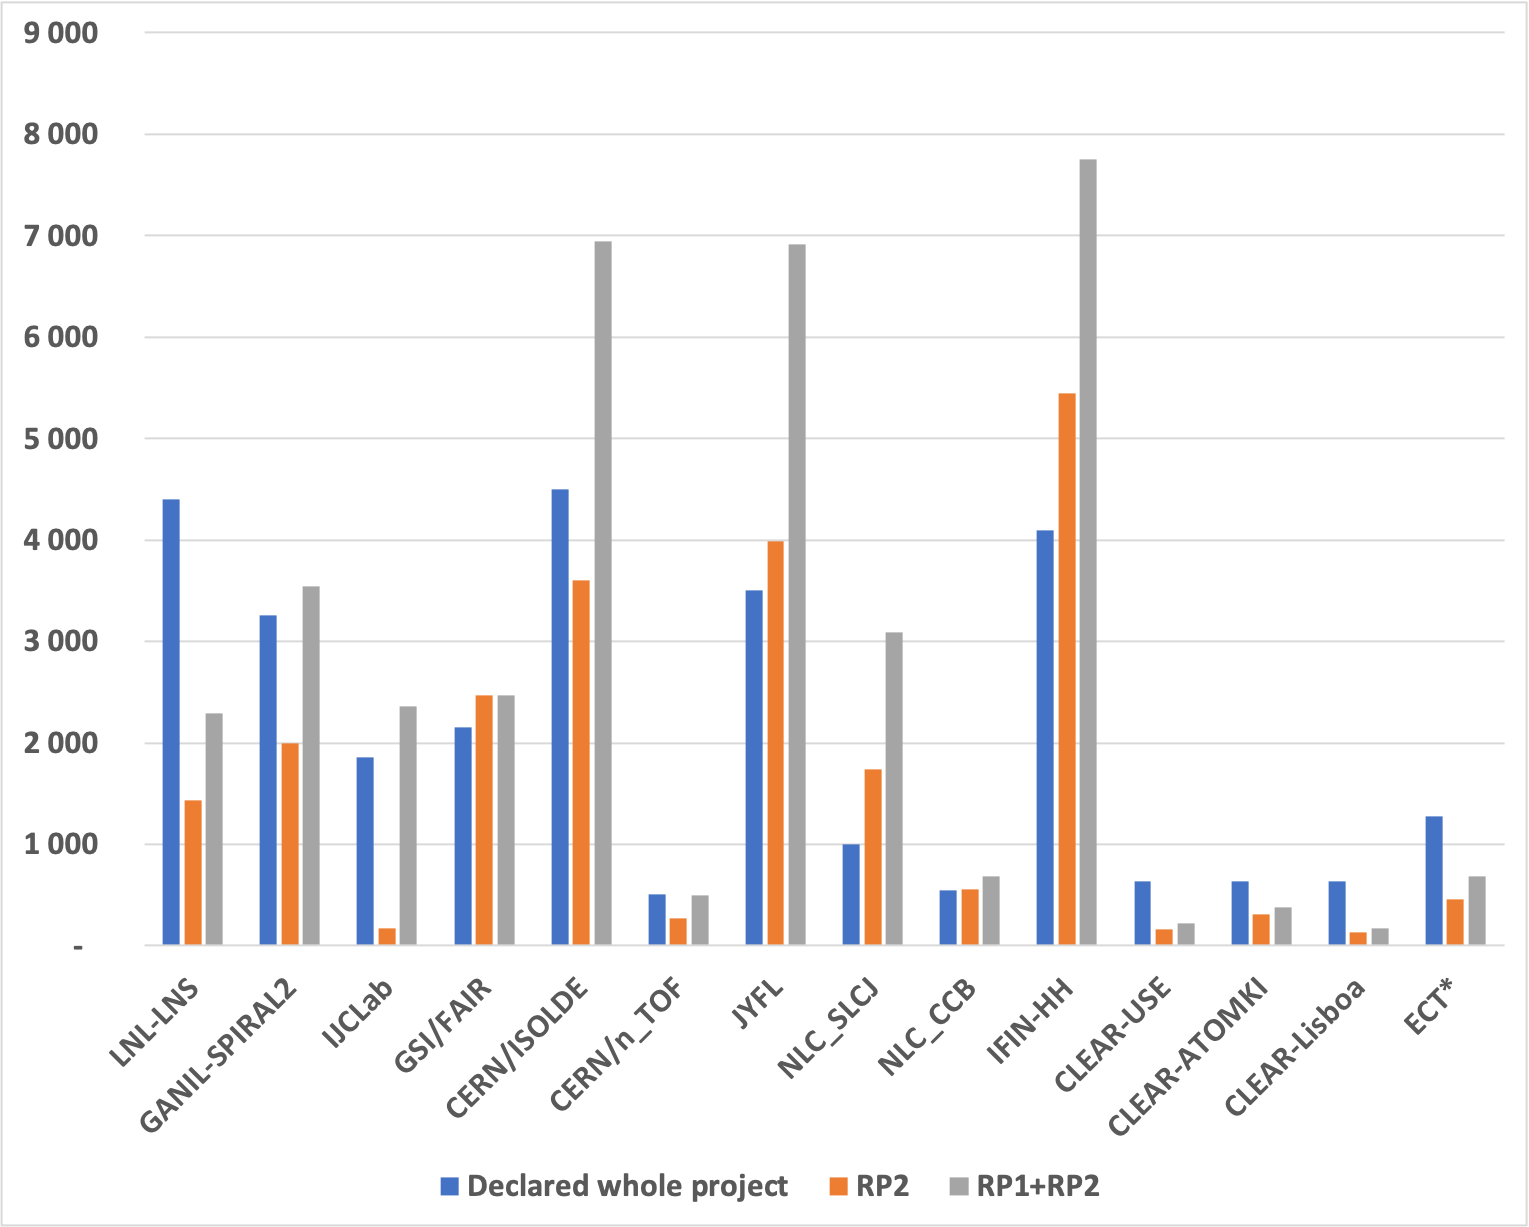
\includegraphics[width=0.8\linewidth]{graphics/WP2_AU_statistics.png}
    \caption{Distribution of the Access Units (hours of the beam time in the case of the beam facilities, or days of visits in the case of ECT*) provided within WP2 facilities in P2}
    \label{fig:WP2_AU_statistics}
\end{figure}

In P2, 194 TA projects were supported: 86 projects in Task 2.1 (Stable ion beams), 82 projects in Task 2.2 (Radioactive Ion beams), 11 projects in Task 2.3 (Neutron beams) and 11 projects for the TA access to the theory center ECT* (cf. Fig.~\ref{fig:WP2_projects}).  In addition, the facilities have exhausted in P2 28\% (which makes 45\% for both P1 and P2) of the allocated Travel and Subsistence (T\&S) funding, supporting traveling expenses and visits of 836 users (with approximately 30\% of female scientists) to prepare and develop instrumentation prior to the actual delivery of the beam, to run the experiments, or visit the theory center ECT*. Details are shown in the Figs.~\ref{fig:WP2_users_per_country} and~\ref{fig:WP2_users_men_women}. 

\begin{figure}[!h]
    \centering
    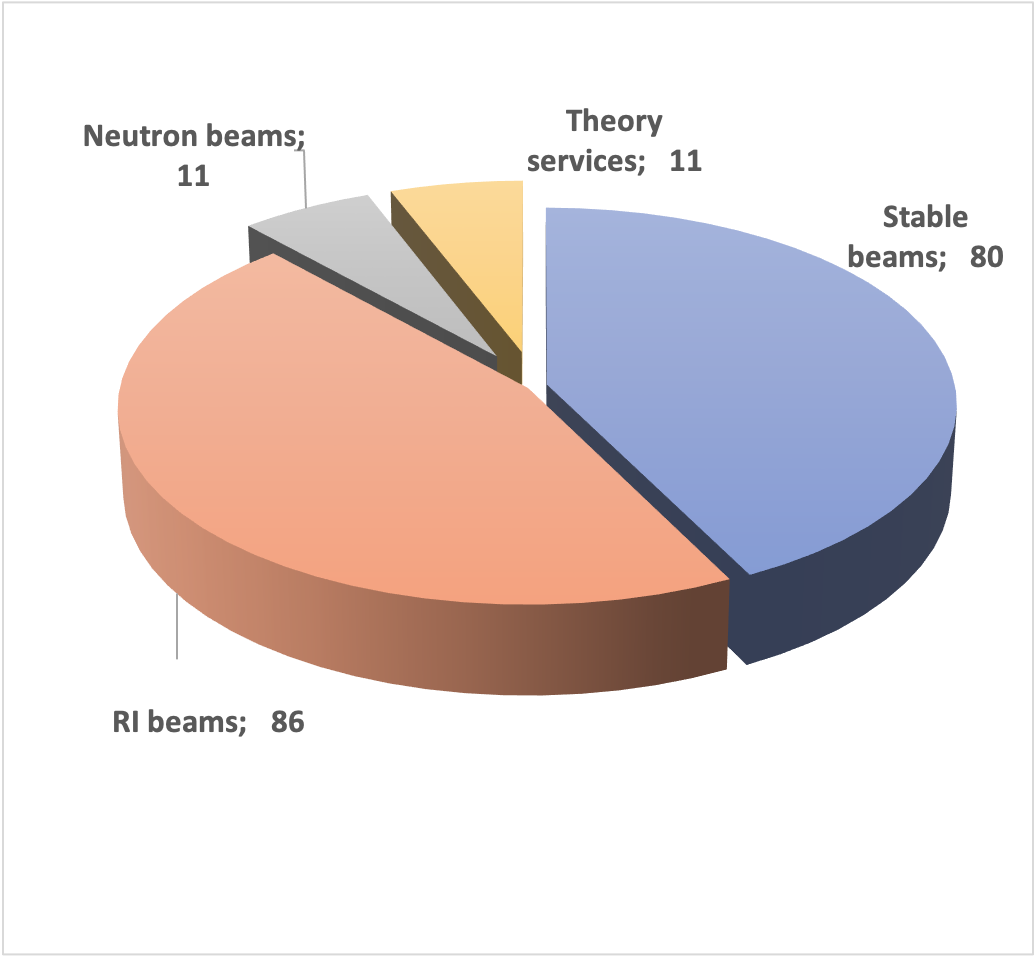
\includegraphics[width=0.95\linewidth]{graphics/WP2_projects.png}
    \caption{Left: TA Projects realized in P2 in different WP2 tasks. Right: Access Units used in P2 in different WP2 tasks.}
    \label{fig:WP2_projects}
\end{figure}


\begin{figure}[!h]
    \centering
    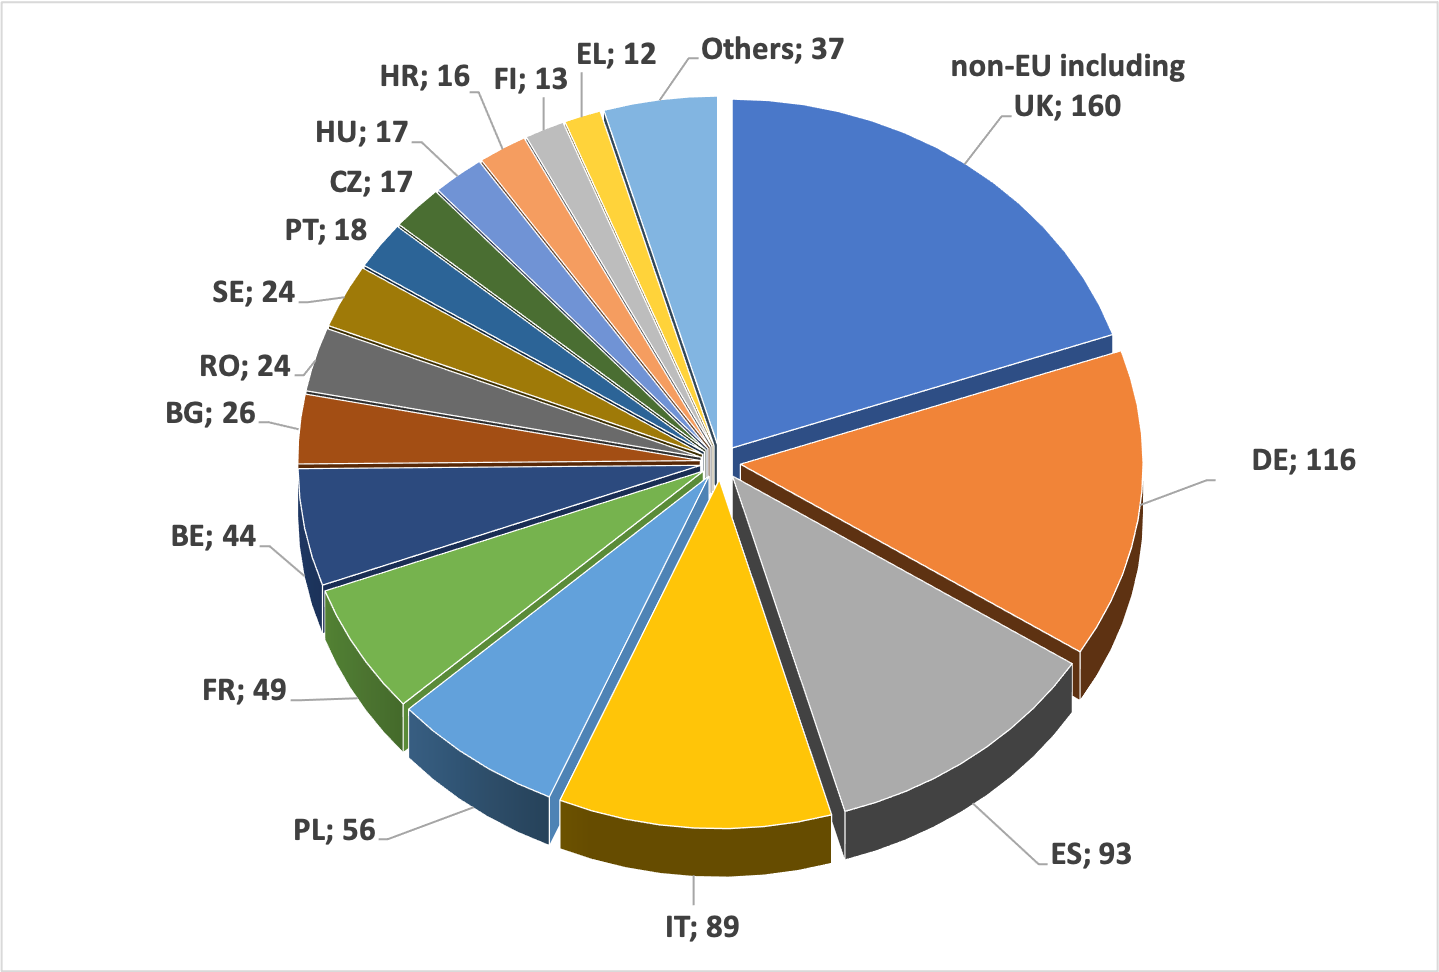
\includegraphics[width=1.0\linewidth]{graphics/WP2_users_per_country.png}
    \caption{Geographical distribution of TA users' home institutions in WP2 during P2.}
    \label{fig:WP2_users_per_country}
\end{figure}

\begin{figure}[!h]
    \centering
    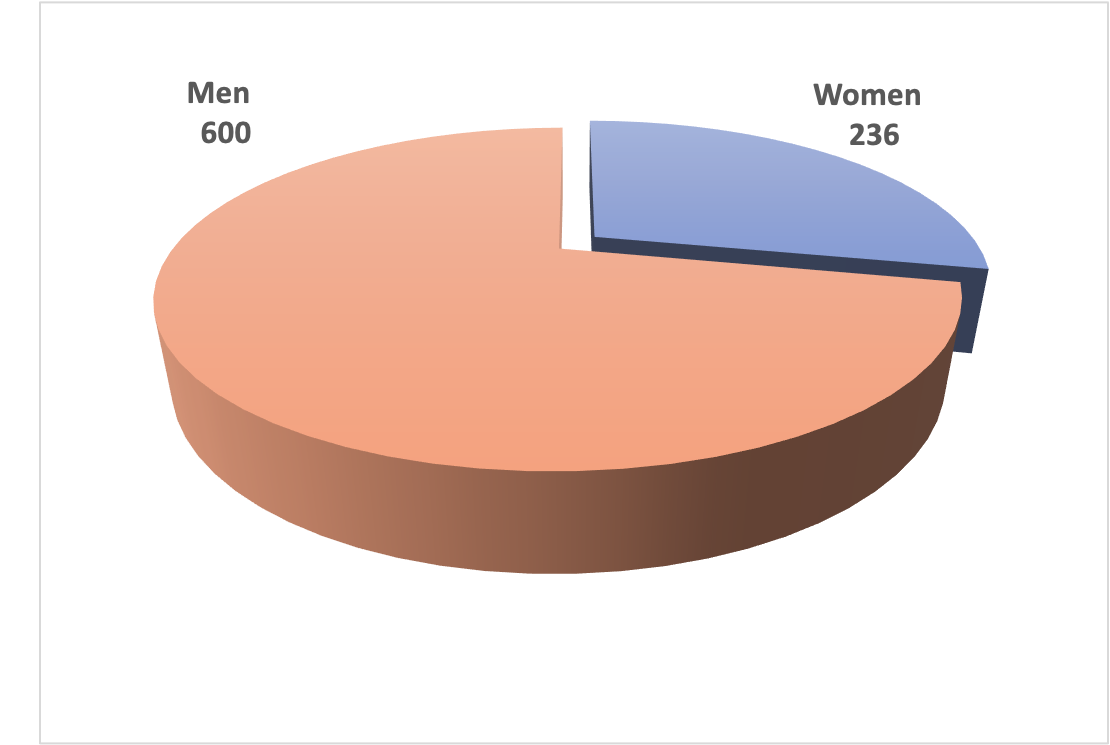
\includegraphics[width=0.6\linewidth]{graphics/WP2_users_men_women.png}
    \caption{Female vs. male distribution of TA users in WP2 during P2.}
    \label{fig:WP2_users_men_women}
\end{figure}


The activities planned in P2 for Service Improvement, related to streamlined and remote access, targets for high intense beams, biomedical applications, improving ion beam services and optimal employment of traveling gamma-ray detectors, are progressing well. 

The synergy between theory and experiments has been secured by the TA offered at the ECT* center, where 11 events were organized, aimed at 
discussing hot topics in the field of nuclear structure and reactions
(microscopic optical potentials, strangeness in nuclear reactions, nuclear theory and reactions for astrophysics, hadron tomography, neutrino interactions, electric dipole moments,  and machine learning). 

Moreover, the new facility (Theo4Exp) offering VA to theoretical tools accessible via user-friendly web pages, to help preparing and interpreting experiments, has been successfully installed and started delivering access.
\subsubsection*{Progress per Task}
\subparagraph{Task 2.1: Stable Ion Beams} \mbox{}

%\todo{Briefly explain the progress of the task in context to the DoA.}

Period 2 has proven to be an extremely busy one for the Stable Ion Beam facilities of Task 2.1. All eight facilities (including consortia) have supported multiple experiments with a very high level of success. A total of 86 were supported in P2.

Whilst still performing the “traditional” forefront experiments in fundamental nuclear physics research, the program of science covered by the Stable Ion Beam facilities is very broad and multidisciplinary. Nuclear and accelerator-based techniques are being also used to address a variety of topics, 
%as far 
ranging from radiation shielding for lunar habitats (GSI-FAIR), radiation effects in 2D Nanostructures (GANIL), effects of heavy ion radiation on cells (GSI-FAIR and GANIL), to thin film elemental characterisation for photovoltaic cells (CLEAR – IST), improved processes for purification of phosphogypsum (CLEAR – IST), assessment of the impact of dumping of radioactive materials in the Baltic Sea region (CLEAR – CNA) and analysis of air quality in the city of Naples (CLEAR – ATOMKI).

It should be noted that a number of experiments which highlight the importance to the community of having a large range of facilities of different scale, offering different ion beams and techniques, with efficient and flexible access available. Novel $^3$He and $^4$He targets, made by magnetron sputtering and trapped in a suitable substrate, were characterised at \textbf{CLEAR-CNA} and subsequently used in fundamental nuclear science experiments at other facilities. For instance, the $^4$He targets were used to study elastic $\alpha$-scattering on heavy nuclei, relevant for nuclear astrophysics, and the $^3$He targets were to be used in the measurement of the lifetime of a subthreshold state in $^{15}$O, produced by neutron transfer from an $^{16}$O beam, using apparta (AGATA and SAURON) installed at INFN-LNL. 
%The $^{15}$O will be produced by neutron transfer to the $^3$He target from an $^{16}$O beam. 
At GANIL, experiments were made to assess the performance of thin, electrodeposited targets for future studies of Superheavy Elements (SHE) using high intensity ion beams. At \textbf{CLEAR-IST}, self-supporting $^{208}$Pb targets were characterised in order to reduce uncertainties in the analysis of Coulomb breakup experiments (to investigate $^6$He, for example). \textbf{CLEAR-ATOMKI}  characterised the tracking capability and sensitivity of detectors which will be used in a forthcoming experiment at the n$\_$TOF neutron irradiation facility at CERN. At \textbf{ALTO}, an in-beam test was made to investigate the high-rate performance of the detectors and read-out chain which will form part of the G-NUMEN gamma-array demonstrator. In future, the NUMEN experiment will be focused on Nuclear Matrix Elements for neutrinoless double beta decay. 

At \textbf{GANIL} eight stable ion beam projects were carried out, supported by 1448 hours of beam time. 

At \textbf{GSI/FAIR}, the NUSTAR collaboration carried out ten experiments during RP2, exploiting 1217 Access Units.  

At the \textbf{IFIN-HH} 24 experimental groups were supported and received 5450 hours of beam time. Data analysis is ongoing for most groups, but several have already published or submitted their results for publication. 

At \textbf{JYFL}, fourteen stable ion beam experiments were supported during the reporting period. The experiments were granted a total of 3096 hours of beam time access. Aside from one experiment which used the TOSCA two-arm time-of-flight spectrometer to study fission dynamics at the Large Scattering Chamber, the recoil separators RITU and MARA 
were employed
to study various aspects of nuclear structure physics and reaction dynamics, in particular Multi-Nucleon Transfer reactions. The efficiency of performing campaigns at the separators, which can house the JUROGAM3 array of germanium detectors at their target positions, has been enhanced by the use of a gantry which allows the array to move from one separator to another within hours (see Fig.~\ref{fig:Jurogam3}). This removes the need to un-bias the detectors before moving the array, which previously resulted in a need to anneal the detectors to repair radiation damage. The latter procedure can take weeks-months. 

\begin{figure}[!h]
    \centering
    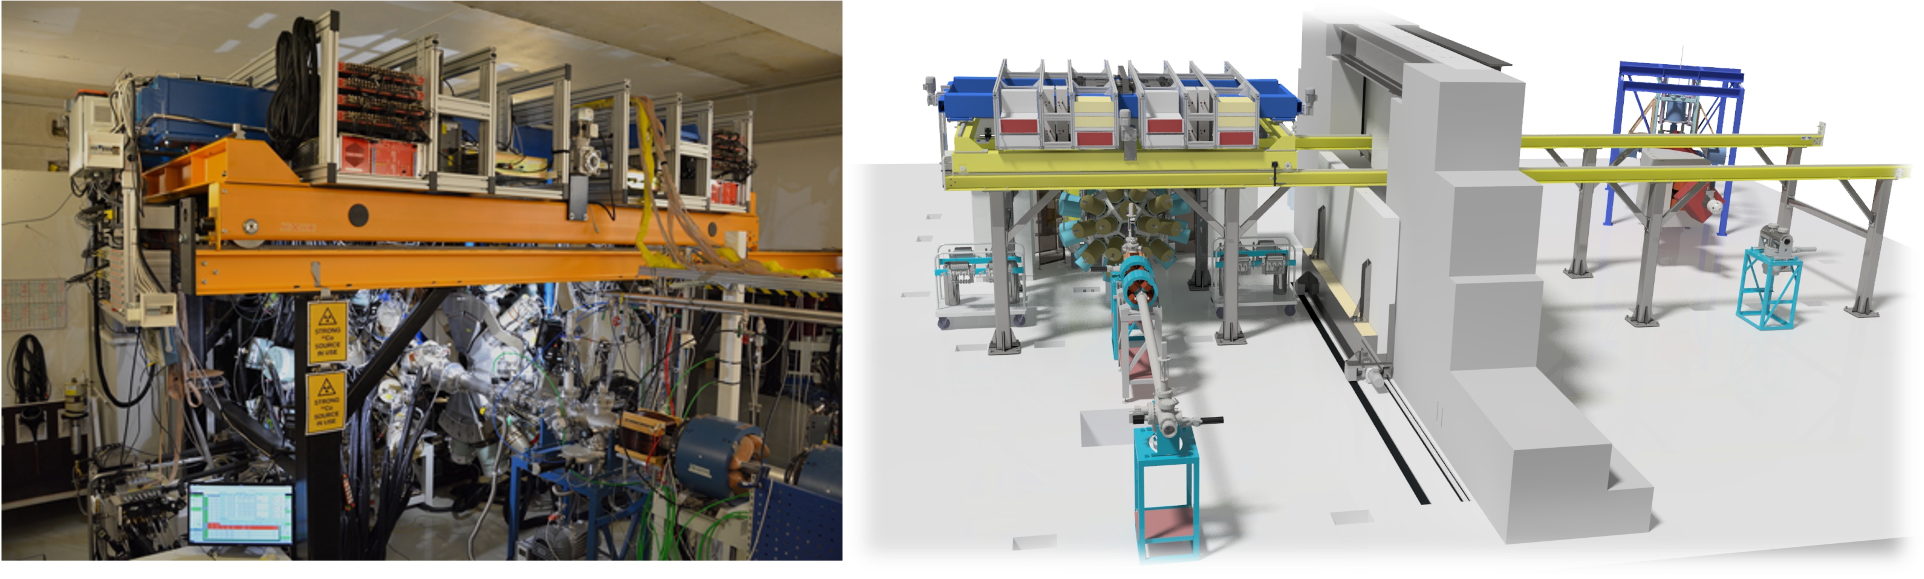
\includegraphics[width=1.0\linewidth]{graphics/Jurogam3.png}
    \caption{The JUROGAM3 array at the target position of the MARA recoil separator and the gantry system to allow rapid relocation of the array to the sister separator, RITU.}
    \label{fig:Jurogam3}
\end{figure}

At \textbf{INFN-LNL}, a total of ten experiments were supported during P2,  using 1431 access units. The experiments exploited the European AGATA gamma-ray tracking array (see Fig.~\ref{fig:AGATA_LNL}) in various configurations with ancillary detectors. Using AGATA-SPIDER, a number of Coulomb excitation experiments were performed to study several aspects of nuclear structure, such as the emergence of collectivity near $^{60}$Ni (experiment 23.008) and the interpretation of the structure of excited 0$^+$ states in $^{106}$Pd (experiment 23.054). AGATA-PRISMA was used, along with RDDS and DSAM techniques, to measure lifetimes in $^{50-52}$Ca and $^{46-48}$Ar, aiming to understand shell evolution close to N=28 and Z=20 (experiment 22.81). The same devices were used to measure Multi-Nucleon Transfer (MNT) reactions. 
 Other devices combined with AGATA for experiments were AGATA-SAURON, AGATA-EUCLIDES and AGATA-OSCAR. This shows the versatility of the devices which can be modified for campaigns of experiments using different complementary techniques.

\begin{figure}[!h]
    \centering
    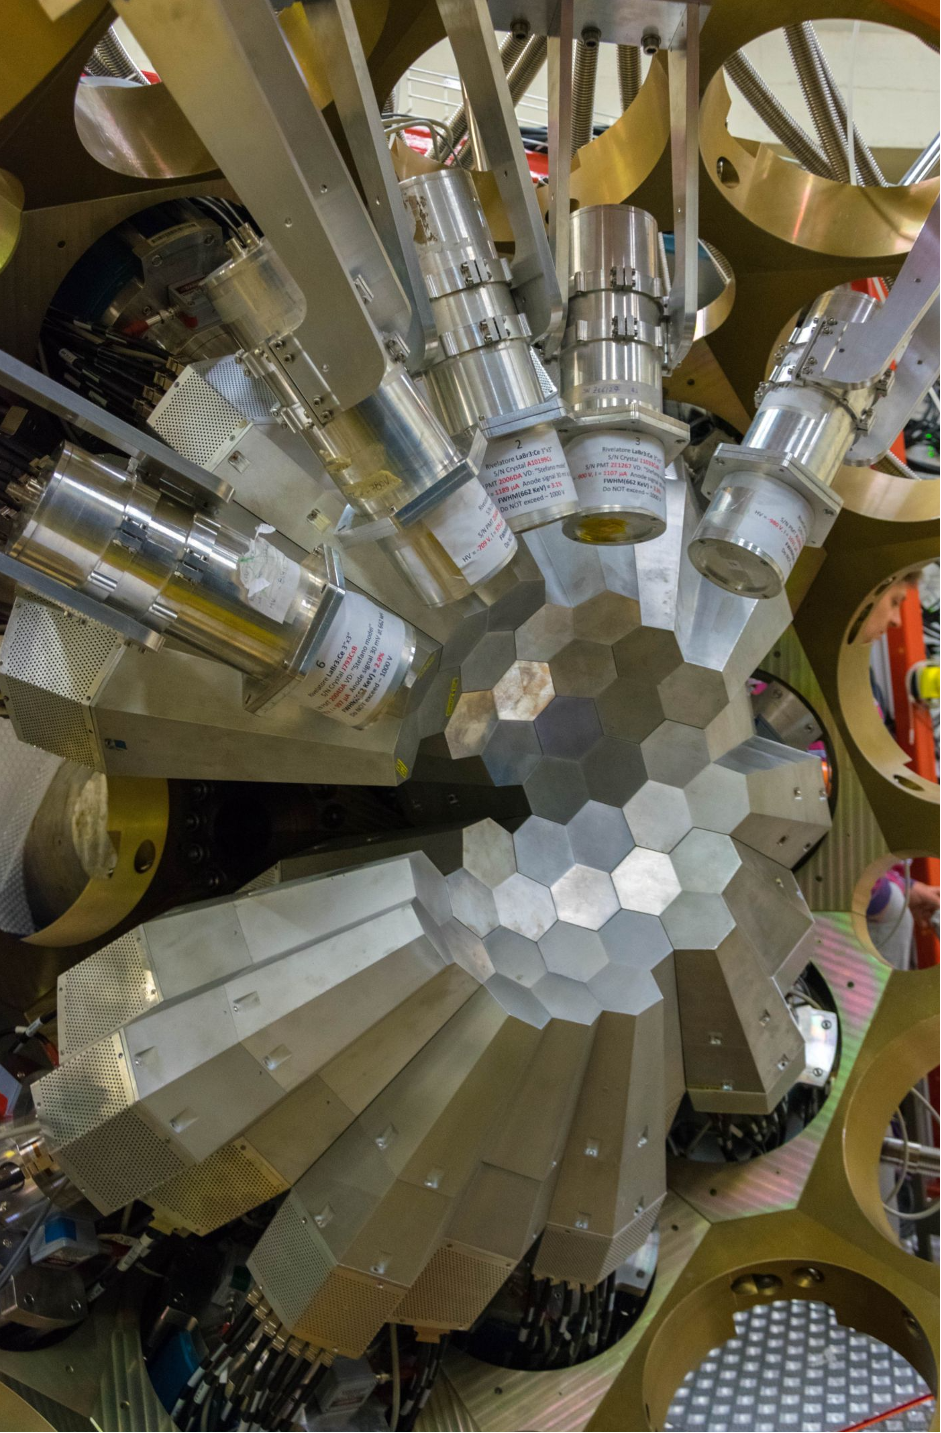
\includegraphics[width=0.5\linewidth]{graphics/AGATA_LNL.png}
    \caption{The European AGATA gamma-ray tracking array installed at INFN-LNL.}
    \label{fig:AGATA_LNL}
\end{figure}

At \textbf{NLC-CCB} (Krakow) two long (lasting few weekends each) experiments were performed, with the use of 560 hours of high energy proton beams. 

At \textbf{NLC-SLCJ} (Warsaw), six supported experiments were carried out, using 1744 hours of beam time.

Only \textbf{INFN-LNS} has not delivered any access time, as it is under re-construction.

\subparagraph{Task 2.2: Radioactive Ion Beams} \mbox{}

%\todo{Briefly explain the progress of the task in context to the DoA.}

Period 2 was also very busy for the Radioactive Ion Beam facilities of Task 2.2. Four facilities have supported 82 experiments in this period, providing almost 6000 hours of RI beams. 

At the \textbf{GANIL-SPIRAL2} facility two projects received Transnational Access during P2, focusing on Nuclear Physics investigations on light radioactive nuclei and exploiting 224 hours of RI beams.

The RI beams at \textbf{GSI/FAIR} are delivered to the nuclear and astrophysics community (NUSTAR). During the P2 period, fourteen user projects have been supported by Transnational Access. 1248 hours of radioactive ion beams were provided. Within these experiments, different setups and parts of the facility were used, such as the experimental storage ring ESR, the R3B ( Reactions with Relativistic Radioactive Beams) experiment, the DESPEC (DEcay SPECtroscopy) detector setup, the FRS (Fragement Seperator) itself, the FRS Ion Catcher and the EXPERT detector. 

%Experiments using FRS recorded a comprehensive dataset for projectile-fragmentation products (Z = 82 to 89) from 238U on a Be target, providing essential data to refine fragmentation models and support future NUSTAR experiments. ESR has been used for investigating the rare double-gamma decay mode in 0$^+$$\rightarrow$0$^+$ transitions, this study measured isolated double-photon decays in $^{72}$Ge, and compared the two-photon decay in $^{98}$Zr and $^{98}$Mo to assess whether enhanced transition rates depend on nuclear structure and measures of de-excitation probabilities over a wide energy range in excited $^{238}$U and $^{239}$U. For the first time, simultaneous measurements of fission, gamma, and multi-neutron emission (up to three neutrons) were achieved in a storage ring setting. R3B setup has been used for commissioning of key detectors (CALIFA, Si-tracker FOOT, NeuLAND). Cross-section measurements for (p,pd) reactions on various carbon isotopes were performed indicating the presence of strongly correlated neutron-proton pairs, with quasi-deuteron behavior influencing nucleon “dressing” in the nuclear medium. DESPEC gathered spectroscopic data around N=126 shell closer, a critical region for r-process nucleosynthesis, where new level schemes and transition probabilities help benchmark models describing the interplay of single-particle orbitals and collective excitations in heavy nuclei relevant for the astrophysical sites. FRS Ion Catcher has been used in three different experiments. A proof-of-principle study using slowed-down uranium beams in a Cryogenic Stopping Cell demonstrated that multi-nucleon transfer (MNT) reactions can produce neutron-rich isotopes (A $\approx$ 160–250). MNT products were successfully extracted and identified with the MR-TOF mass spectrometer, paving the way for future RIB production at Super-FRS. Also focusing on exotic nuclei from Br to Rh, this study addresses issues such as isospin symmetry breaking, the Wigner effect, and unexpected mass discrepancies (e.g., $^{70}$Br). The FRS Ion Catcher, combined with a $^{107}$Ag fragmentation beam and SIS-18 accelerator mode, delivered precise mass measurements, essential for validating nuclear models and rp-process calculations. EXPERT detector using a $^9$C beam, the experiment probes Thomas-Ehrman shifts in mirror pairs (e.g., $^5$H-$^5$Be, $^6$H-$^5$B, $^7$H-$^7$C) and measures decay energies, widths, and half-lives (down to picoseconds) via multi-particle angular correlations. Upgraded high-rate tracking detectors have enabled high-statistics data collection, allowing for improved measurements of nuclear state widths and the identification of novel multi-proton decay mechanisms.

At \textbf{JYFL} a total of six supported experiments were carried out using 888 hours of beam time access. %through Transnational Access during EURO-LABS P2. 

At the \textbf{CERN/ISOLDE} facility, 64 projects received Transnational Access during P2, focusing on Nuclear Physics investigations, and using 3604 hours of beam time.

\textbf{LNL/LNS} and \textbf{ALTO} had no Radioactive Ion Beams projects receiving Transnational Access during P2.

\subparagraph{Task 2.3: Neutron Beams} \mbox{}

%\todo{"Briefly explain the progress of the task in the context to the DoA"}

In P2, four neutron beam facilities supported 11 project, providing altogether more than 700 hours of neutron beams.

At CERN's \textbf{n\_TOF} facility, seven projects were granted Transnational Access during the EURO-LABS P2 phase, focusing on various nuclear physics investigations and exploiting 271 hours of beam.

At \textbf{CLEAR-CNA} one project using neutron beams was supported, with 48 hours of beam provided.

At the \textbf{ALTO} facility, one project using 72 hours of neutron beams from the LICORNE facility was supported.

At \textbf{GANIL-SPIRAL2} the NFS facility offered 328 hours of neutron beam to 2 projects.

\subparagraph{Task 2.4: Theoretical Support} \mbox{}

%\todo{Briefly explain the progress of the task in context to the DoA.}

Theoretical support for experimental activities was enhanced in P2 following two subtasks. 

WP 2.4.1 enables in-person \textbf{TA to ECT*} (the European Centre for Theoretical Studies in Nuclear Physics and Related Areas, Trento). During P2, ECT* hosted 30 workshops and one Doctoral Training Program (DTP), following calls for proposals in the spring and summer of  2023 and 2024. Calls are made through the ECT* website (\url{https://www.ectstar.eu}) and the extensive mailing list of ECT* associates. In addition, the ECT* Director and the Scientific Board actively solicit proposals to ensure a balanced annual program.
Among the successful proposals, the Scientific Board, which serves as User Selection Panel for EURO-LABS, selected for P2 10 workshops and the 2024 DTP.  A highlight was the DTP, which introduced students from different backgrounds in nuclear physics and astrophysics to the current state of the art in the field of nuclear astrophysics, regarding in particular new constraints on the equation of state of neutron-rich matter from nuclear theory, experiments, and observations, core-collapse supernovae as the birthplace of neutron stars, and mergers and gravitational waves as probes of the neutron-star interior. 
In the P2 period, ECT* provided access to 105 EURO-LABS users, using 479 Access Units (i.e. days spent by users in ECT*). In addition, the Scientific Board has selected EURO-LABS activities for the remainder of 2025, promoting workshops on several hot topics in nuclear physics.  
Among future activities, a highlight is a workshop in support of the Virtual Access provision in WP 2.4.2. 


WP 2.4.2 provides access to theoretical tools through the \textbf{virtual-access infrastructure Theo4Exp}. This VA service has been available since 1 February 2024 at \url{https://institucional.us.es/theo4exp}. Its opening to users has been posted in the EURO-LABS webpage and in social media, as well as distributed widely via mailing lists. The infrastructure consists of three installations: MeanField4Exp at IFJ PAN Kracow, Reaction4Exp at University of Sevilla, and Structure4Exp at University of Milano. The link to each installation can be easily found in the main webpage. User access to the installations is provided by the application \url{https://iam-eurolabs.ijclab.in2p3.fr/login}, which has been developed by WP5 of the present EURO-LABS project. This application ensures access to any researcher affiliated with a scientific institution via either eduGAIN (\url{https://edugain.org/}) or ORCID (\url{https://orcid.org/}).
An International Review Panel (IRP) meets every year to review and validate the progress made on the VA infrastructure and its three installations. The IRP is composed by P. Bednarczyk (IFJ-PAN, Chairperson), A. Moro-Mu\~noz (University of Seville), E. Vigezzi (INFN-Milano), K. Rusek (University of Warsaw), I.J. Thompson (Lawrence Livermore National Laboratory, LLNL), and A. Gargano (INFN-Napoli). Two meetings have been held in the reporting period P2, on 20th September 2023 and 10th October 2024. An article about Theo4Exp has appeared in the first 2025 issue of Nuclear Physics News 
(\url{https://www.tandfonline.com/doi/epdf/10.1080/10619127.2025.2454884}). 
A hands-on workshop, aimed at an optimal use of the Theo4Exp installations, is scheduled for July 2025 at ECT* (\url{https://www.ectstar.eu/workshops/theory-service-for-the-low-energy-nuclear-physics-community-a-hands-on-workshop/}).
In P2 13 projects (virtual services) were offered and realized by 188 remote users. In total 1915 Access Units (counted as each started hour of active use of the virtual service) were provided . These numbers are almost twice higher as estimated for the whole duration of the project.


\subparagraph{Task 2.5: Service Improvements } \mbox{}

%\todo{Briefly explain the progress of the task in context to the DoA.}

This task is divided into 5 different activities. A short summary of the latest progresses is provided below.

\underline{WP2.5.1 Streamlined and remote access:} 

a) In the Streamlined Access part of the subtask, the offer of facilities providing beam for nuclear physics research within the WP2 package is presented in a more uniform and detailed way  through the website (still under construction) \url{https://www.slcj.uw.edu.pl/en/tna-euro-labs/}. Each facility has its own subpage with a menu that provides easy access to specific information, such as: site details, list of available infrastructures and beams, beam time schedule, application submission deadlines and details, meeting dates of Program Advisory Committies, total number of access units in use and still available, access procedures, details about the TNA support and the application process, and a list of publications. 

b) The Remote Access part of the subtask aims to provide improved remote access to EURO-LABS institutions (i.e., any kind of accessibility to experimental operation from outside of experimental areas, for locals experts and external participants). The main goals are to minimise required access to experimental areas and travel time for on-call experts, thus maximising external participation, and standardise generally-endorsed approaches and procedures. This subtask is divided into three main categories: i) the development of a user-friendly database to disseminate information on remote-access tools currently in use at EURO-LABS facilities, ii) the implementation of new/improved remote-access tools at EURO-LABS facilities, and iii) provide training opportunities to the community. The completion of part i) was reported in EURO-LABS project milestone M12 in February 2024. The database is fully operational (available here: \url{https://eurolabs-remote.gsi.de/}) and the collection of further information to expand the content is underway. A set of tools to provide remote control of the experimental irradiation setup are being implemented at the PARTREC facility, with the aim of minimising the amount of personnel needed on-site for guest research groups and/or paying customers of the PARTREC cyclotron.
To avoid potential security issues, users will not get direct access to the irradiation control system. Rather, they will receive access (via VPN) to an interface PC connected to the (less privileged) internal network.
A Python server running in the irradiation control PC parses the user’s input, and translates them into operations for the irradiation control system written in Labview, via the ActiveX interface. The server code will be open sourced in the near future.
With the aim of advertising the "Remote Handling" database, a half-day workshop has been organised as a satellite meeting to the "VIIth Topical Workshop on Modern Aspects in Nuclear Physics" conference on Feb. 4th, held in Bormio (Italy). 


\underline{WP2.5.2 Targets for high intense beams:} A database containing information on the preparation and characteristics of the targets available at the participating institutions, as well as those newly developed as part of this subtask, has been completed. In particular, with the post-docs hired with EURO-LABS funds at INFN-LNS and at GANIL, we collected information on the produced targets, their characteristics and manufacturing techniques from the collaborating institutions and the literature. The first version of this database is now ready and will be made public in the coming months via a user-friendly application.

\underline{WP2.5.3 Biomedical application (FLASH@EURO-LABS):} Air-filled Farmer-type ionization chambers are widely used as standard detectors for absolute dosimetry in clinical settings. However, under Ultra-High-Dose-Rate (UHDR) conditions, these chambers experience significant recombination effects, resulting in high uncertainties in dose measurements.
The progress in this task was in 3 different topics: 1. Development and Benchmarking of a Numerical Model for Farmer-Type Ionization Chambers (cf. Fig.~\ref{fig:FLASH1}); 2. Application of the Developed Numerical Model: Evaluating the Reliability of the TM31023 Detector for Carbon Ion FLASH Applications; 3. Improvement of Dosimetry Uncertainty at Clinical Facilities. Results are summarized in the report of MS14.


\begin{figure}[!h]
    \centering
    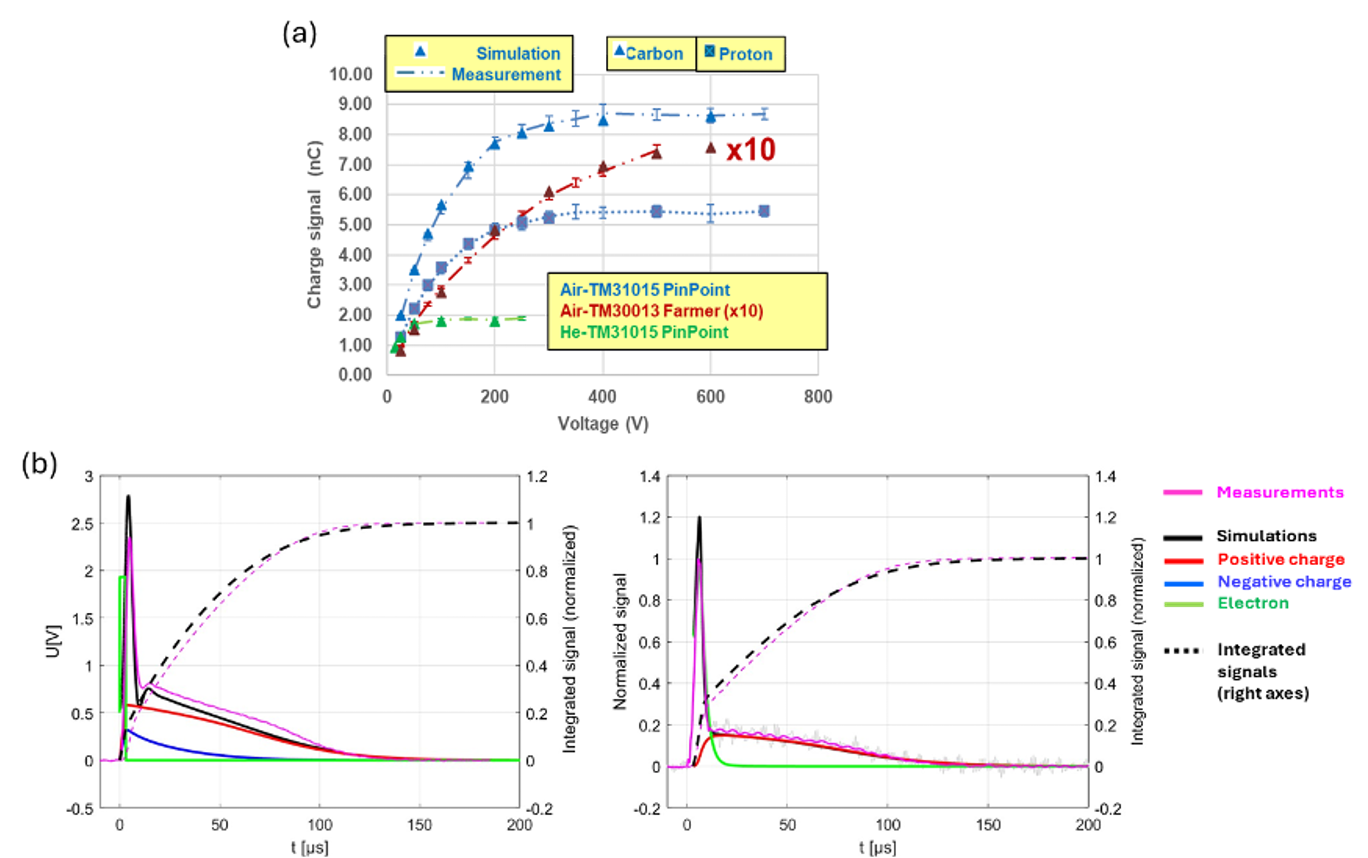
\includegraphics[width=1.0\linewidth]{graphics/FLASH1.png}
    \caption{Comparison of simulation and experimental data for FLASH dosimetry:
(a) Saturation curves of 3 different ionization chambers irradiated with protons at ultra-high dose rate at HIT (Heidelberg Ion-Beam Therapy Center) in Heildeberg. (b) Time-resolved signals of the ionization chamber, whose integral corresponds to the charge collected by the electrometer, measured using a pulsed LINAC at Universitätsklinikum Gießen und Marburg (UKGM) at ultra-high dose rate. The signals from air-filled and nitrogen-filled Farmer chambers exhibit distinct differences in shape. This variation arises from the absence of electronegative molecules, such as oxygen, in the nitrogen-filled chamber, which prevents electron attachment.
}
    \label{fig:FLASH1}
\end{figure}

\underline{WP2.5.4 Improving Ion Beam services in variety and stability (ERIBS):} The project has been divided into two separate parts to achieve the objectives. Part 1 focuses on extending the ion beam selection and intensities to allow new projectile-target combinations and/or make low-cross section reaction studies possible. Part 2 focuses on developing online beam monitoring to maintain the requested beam intensity. In Part 1 the main progress was in the MIVOC service and technology transfer. In Part 2 progress was done in optical emission spectroscopy and online beam intensity monitoring.

\underline{WP2.5.5 Optimal employment of traveling gamma detectors (INTRANS):} The INTRANS (Instrumentation and Training for Nuclear Spectroscopy and Reaction Dynamics) subtask has organized and/or sponsored a series of events since September 2023, including: Two AGATA Analysis workshops; InTraNS Workshop; Gamma Detectors Hands-on Training on operation, test and repair of Hyper Pure Ge Detectors; InTraNS Training Workshop on Coulomb Excitation (see MS16). 

The work in all of the Service Improvements tasks is progressing according to the plan and shall be finished by the Month 36 of the EURO-LABS project.


\subsubsection*{Main Results and Achievements}

%\todo{Briefly summarise the main results and achievements of the DoA in context of the DoA.}

Progress in the TA offer in Tasks 1-3 is described above. 

Concerning Task 2.4, 
the main achievement was the opening to external users, in February 2024, of the Virtual Access facility Theo4Exp. All three components of Theo4Exp have implemented theoretical tools for the evaluation of experimental data. MeanField4Exp at IFJ PAN KraKow now offers mean-field predictions for the evolution of nuclear shape with angular momentum, as well as the effects of deformation and shape on single-particle and potential energies. Reaction4Exp, now online at University of Sevilla, enables the calculation of Coulomb breakup, elastic and inelastic scattering, and transfer reactions. Structure4Exp at University of Milano provides properties like masses and radii for ground and excited nuclear states from self-consistent mean-field methods and the Shell Model. In addition, collaborations between theorists and experimentalists were stimulated by 10 workshops and an advanced school hosted by ECT* (Trento), covering various aspects of nuclear structure, reactions and astrophysics, as well as strong and weak interactions, fundamental symmetries, high-power lasers, and machine learning.

The main achievements for task 2.5 in the P2 period are: i) the delivery of a new website in WP2.5.1; ii) a set-up for reduction and deposition in one-step of rare earth targets in WP2.5.2; iii) the reduction of dosimetry uncertainty to <0.15\%, significantly improving accuracy, in proton therapy centers using Farmer-type ionizing chambers for FLASH in WP2.5.3; iv) the use of optical emission spectroscopy as a real-time monitoring to provide early indications about plasma instabilities in ERIBS; v) the success of the INTRANS workshop, to the point that the INTRANS steering committee decided to hold an additional workshop towards the end of the EURO-LABS contract.





\subsubsection*{Deviations and Corrective Actions}
\label{sec:wp2-deviations}
There are two deviations - one positive, the other negative. The "positive" deviation of the project is that many TA facilities are delivering much more Access Units that planned, some of them already delivered more AU then declared for the whole project. The extra cost of the beam time is covered by the own facilities budget. So no corrective action is required.
The "negative" deviations from the originally planned schedule is slower spending, in some of the WP2 facilities, of the T\&S support. As the corrective action discussions of the EURO-LABS Steering Committee with the Facility Coordinators and corresponding UPS have started. As the result some simplifications of the ministrative procedures for the reimbursement are planned.  

% \todo{Briefly summarise any deviations and performed corrective actions of the DoA in context of the DoA.}

\subsubsection*{Milestones and Deliverables}
In the P2 reporting period, WP2 had five milestones to submit, which have been fully achieved.
{\fontsize{9}{11}\selectfont
\begin{center}
  \begin{tabular}[t]{!{\color{mygray}\vrule}p{0.10\linewidth}!
  {\color{mygray}\vrule}p{0.60\linewidth}!
  {\color{mygray}\vrule}p{0.20\linewidth}!{\color{mygray}\vrule} } \hline
    \rowcolor{mycyan} & {\bf Title} & {\bf Status} \\ \hline
    \cellcolor{mycyan}{\bf MS8}: &Calls for proposals to be hosted at ECT*&  Achieved - \href{https://web.infn.it/EURO-LABS/wp-content/uploads/2024/05/EURO-LABS_MS8-Final-1.pdf} {link}  \\ \hline
    \cellcolor{mycyan}{\bf MS10}: & Contracted personnel for Theo4Exp VA in place and first codes available for users in the virtual facility & Achieved - \href{https://web.infn.it/EURO-LABS/wp-content/uploads/2024/05/EURO-LABS_MS10_The4Exp_02_2024_FINAL-1.pdf}{link} \\ \hline    
    \cellcolor{mycyan}{\bf MS12}: & Completed database containing selected features of remote-access toolkit & Achieved - \href{https://web.infn.it/EURO-LABS/wp-content/uploads/2024/05/EURO-LABS_MS12-Report-RemoteAccess_Final.pdf}{link} \\ \hline 
    \cellcolor{mycyan}{\bf MS14}: & Reports on FLASH detectors for different facilities & Achieved - \href{https://web.infn.it/EURO-LABS/wp-content/uploads/2024/05/EURO-LABS_MS14_Report.pdf}{link} \\ \hline 
    \cellcolor{mycyan}{\bf MS16}: & 	Organisation of hands-on workshops and training schools & Achieved - \href{https://zenodo.org/records/15039933}{link} \\ \hline 
  \end{tabular}
\end{center}
}

\subsubsection*{Project Meetings}
\begin{table}[H]
    \centering
    \caption{Summary of WP2 meetings in P2 and discussed subjects.}
    \begin{tabularx}{\textwidth}{|c|L{0.3\textwidth}|X|} \hline
        \rowcolor{mycyan}
        \textbf{Date} & \textbf{Meeting \& Place} & \textbf{Subject} \\ \hline
        2023-10-09 & WP2 Task Leader's meeting in Krakow & Regular meeting \& progress report \\ \hline 
        2023-10-10 & General WP2 collaboration meeting in Krakow & Status of the project \& progress report \\ \hline         
        2024-08-26 & WP2.4 Collaboration meeting at the Zakopane conference &  Status of the Theo4Exp VA facility \\ \hline
        2024-10-28 & WP2 Task Leader's meeting  at CERN &  Regular meeting \& progress report \\ \hline
        2024-10-30 & General WP2 collaboration meeting at CERN & Status of the project \& progress report \\ \hline
        2024-11-5 & WP2 Collaboration meeting at the SSNET24 conference in Orsay &   Status of the project \& progress report \\ \hline  
        2024-09-25 & WP2.5 Collaboration meeting at the Bormio conference & Service improvements status \& progress report \\ \hline
    \end{tabularx}
    \label{tab:meetings}
\end{table}

In addition, several ad-hoc meetings with the facility coordinators and task leaders were organized via zoom, when it was necessary. 

%  {\color{mygray}\vrule}p{0.40\linewidth}!







%%%%%%%%%%%%%%%%%%%%%%%%%%%%%%%%%%%%%%%%%



%%%%%%%%%%%%%%%%%%%%%%%%%%%%%%%%%%%%%%%%%
%%% WP01
%%%%%%%%%%%%%%%%%%%%%%%%%%%%%%%%%%%%%%%%%

\tsubsubsection{WP03 - Access to RI for Accelerators}

%%%%%%%%%%%%%%%%%%%%%%%%%%%%%%%%%%%%%%%%%
%%% Section content, please change!
%%%%%%%%%%%%%%%%%%%%%%%%%%%%%%%%%%%%%%%%%

\subsubsection*{Overview and Goals}

% --- Data taken from Grant Agreement page 59

\begin{table}[H]
    \renewcommand{\arraystretch}{1.50}		
    \footnotesize   
    \begin{tabular}{*{3}{|p{0.10\textwidth}}|l|}
        \hline
        \rowcolor{mygray} \multicolumn{4}{|c|}{\textit{\color{white}Work Package Summary}} \\
        \hline
        \rowcolor{mylightergray} \textit{WP No.} & \cellcolor{white} 3 & \textit{Title of WP} & \cellcolor{white} (TA2): Access to Research Infrastructures for Accelerator R\&D \\
        \hline
        \rowcolor{mylightergray} \textit{Start} & \cellcolor{white} M1 & \textit{End} & \cellcolor{white} M48 \\
        \hline
        \rowcolor{mylightergray} \multicolumn{4}{|p{0.978\textwidth}|}{\textit{Participating Organisations}} \\
        \hline
        \multicolumn{4}{|p{0.978\textwidth}|}{
            \hspace*{-0.75cm} 
            \begin{minipage}[t]{\textwidth}
    			\begin{itemize}
    			    \item WP Leader: 3 CERN
    				\item Participants: CERN, UU, CEA, CNRS, KIT, INFN, INCT, UKRI
    			\end{itemize} 
    			\vspace*{0.10em}
			\end{minipage}
        } \\
        \hline
    \end{tabular}
    \vspace{0.5em}\vfill
    \begin{tabular}{|p{0.978\textwidth}|}
        \hline
        \rowcolor{mylightergray} \textit{Goals} \\
        \hline
        \rowcolor{white} 
        \hspace*{-0.75cm} 
        \begin{minipage}[t]{\textwidth}
        {\leftskip=15pt
        The work-package groups leading Research Infrastructures (RIs) offering trans-national access related to accelerator
R\&D across Europe.
    		\begin{itemize}
    		    \item Task 3.1 – (TA) for Material testing, lead by CERN

    			\item Task 3.2 – (TA) to Technology infrastructures, lead by CEA

			    \item Task 3.3 – (TA) to Electron and plasma beams, lead by UKRI-
                    \item Task 3.4 – (TA) for TA related to Applications, lead by INCT
    		\end{itemize} 
    		\vspace*{0.10em}
        }
	\end{minipage}        
        \\
        \hline
    \end{tabular}
    \vspace{0.5em}\vfill
    \resizebox{\textwidth}{!}{%
    \begin{tabular}{|l|*{8}{>{\centering\arraybackslash}p{0.084\textwidth}|}}
        \hline    
        \rowcolor{mylightergray} \textit{Participant number} & \textit{1} & \textit{2} & \textit{3} & \textit{4} & \textit{5} & \textit{6} & \textit{7} & \textit{8} \\
        \hline
        \rowcolor{white} \cellcolor{mylightergray}\textit{Participant short name} & CERN & UU & CEA & KIT
                                                                                  & INFN & INCT & UKRI & CNRS \\
        \hline
        \rowcolor{white} \cellcolor{mylightergray}\textit{PM per participant~\footnotemark} & 16.5 & 20 & 20 & ?? & 21 & 16 & 6 & 13\\
        \hline        
    \end{tabular}
    }
\end{table}
\footnotetext{the PM figures correspond to the full duration of the project.}

\subsubsection*{Status}

\begin{figure}[!h]
    \centering
    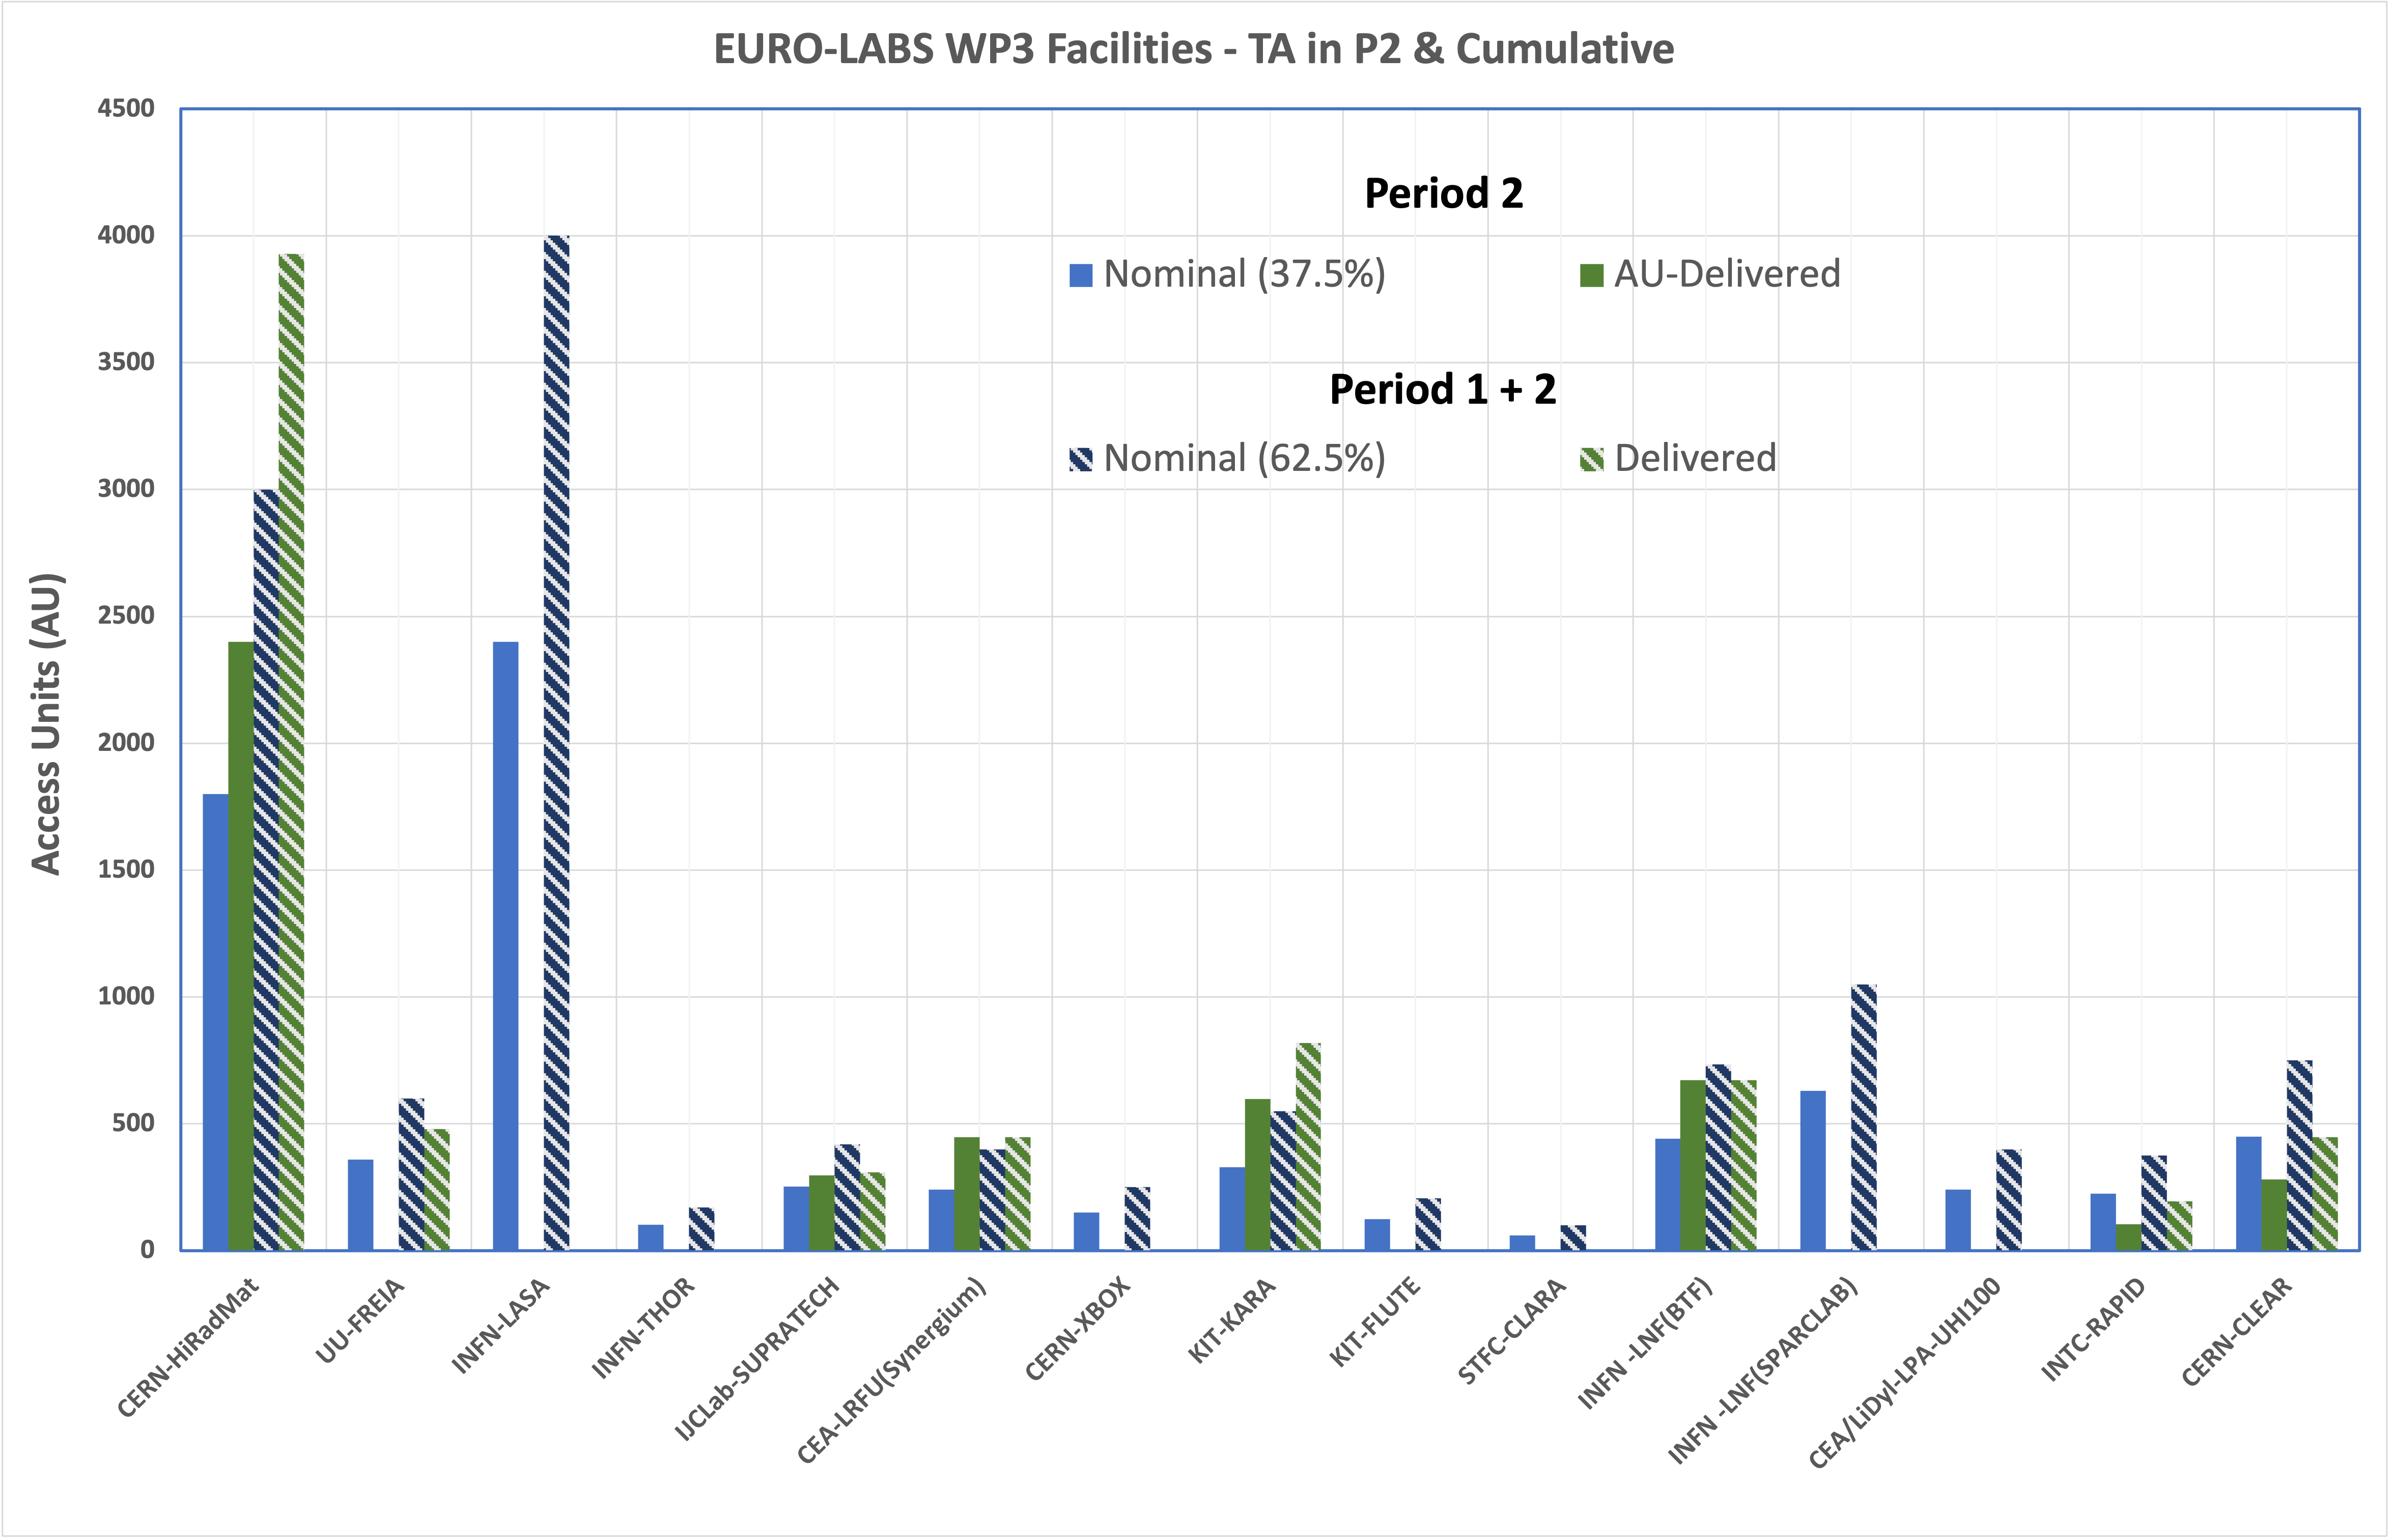
\includegraphics[width=0.98\linewidth]{graphics/WP3-TAstatistics.png}
    \caption{Distribution of AU (typically hours of beam time) delivered in P2 and cumulative for the full duration of the project. The values in the Nominal column represent the fraction of AU for the 18 months of the P2 (37.5\%) or to the 30 months for P1 and P2 (62.5\%) assuming a linear profile.}
    \label{fig:wpe-taunits}
\end{figure}
Over the 18 months covered in P2, the WP3 TA facilities have generally been rather successful in achieving the delivery of transnational access to users. Overall 4799 AU were delivered during P2, representing 84\% of an assumed linear fraction for these 18 months of the AU promised in the GA. The cumulative total for P1 and P2 raises to 7297 AU delivered, corresponding to 56\% of the total number of planed AU for the duration of hte project. This may sound small, however factoring out the facilities where technical or administrative hurdles impacted their capacity to deliver AU, this raises to 78\% which is well within expectations for this stage of the project. The distribution of the AU delivered per TA faciliy is shown in Fig~\ref{fig:wpe-taunits}.

The imbalance between facilities that have exceeded expectations in delivering transnational access (TA) units and those that have experienced inactivity has been thoroughly discussed during the Task and WP meetings. It was agreed that progress will continue to be closely monitored over the coming months. In parallel, a plan has been developed involving a reshuffling of project resources between facilities. This strategy aims to provide additional support to high-demand facilities and ensure the smooth operation of TA delivery for the benefit of the Users.

Beyond transnational access, steady progress has been achieved in the service improvements planned for eight facilities. In most cases, the implementation is ongoing, with the goal of completing these improvements and making them fully operational for the Users before the end of the project.

% \todo{Briefly explain the status of the WP.}

\subsubsection*{Progress per Task}

\subparagraph{Task 3.1 Material Testing Facilities} \mbox{}

This task includes only the HiRadMat Facility at CERN. 

\subparagraph{HiRadMat at CERN}

HiRadmat has had great progress in the last reference period concerning EURO-LABS. The facility remains in extremely high demand from the international community, involving both EU and overseas teams that are performing experiments. A total of 3928 AUs have been spend (from the total requested 4800). The percentage of AUs spent vs the available AUs and the evolution since the start of the project is shown in Figure~\ref{fig:wp3-hrmt-stat}. With the updated schedule of CERN, the facility will remain operational in 2026, the last year of EURO-LABS, and could welcome additional TA requests, also in view of the long shutdown 2026-2029. 
\begin{figure}[!h]
    \centering
    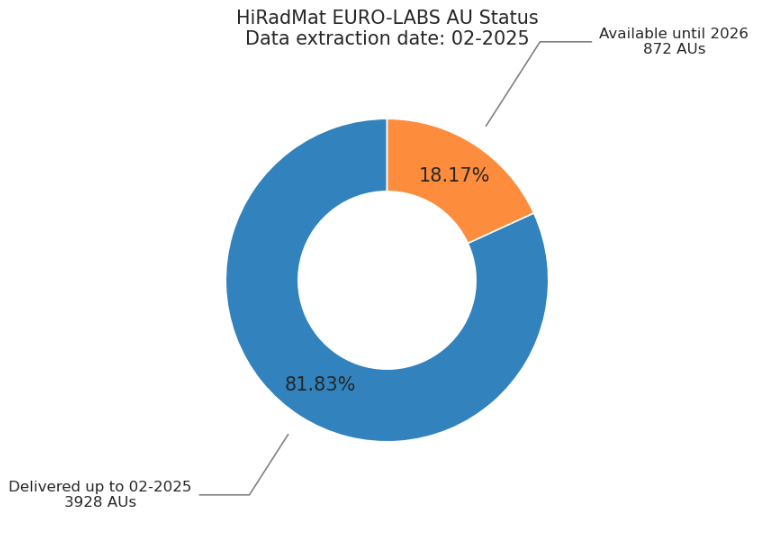
\includegraphics[width=0.48\linewidth]{graphics/stat_pie_hiradmat.png}
    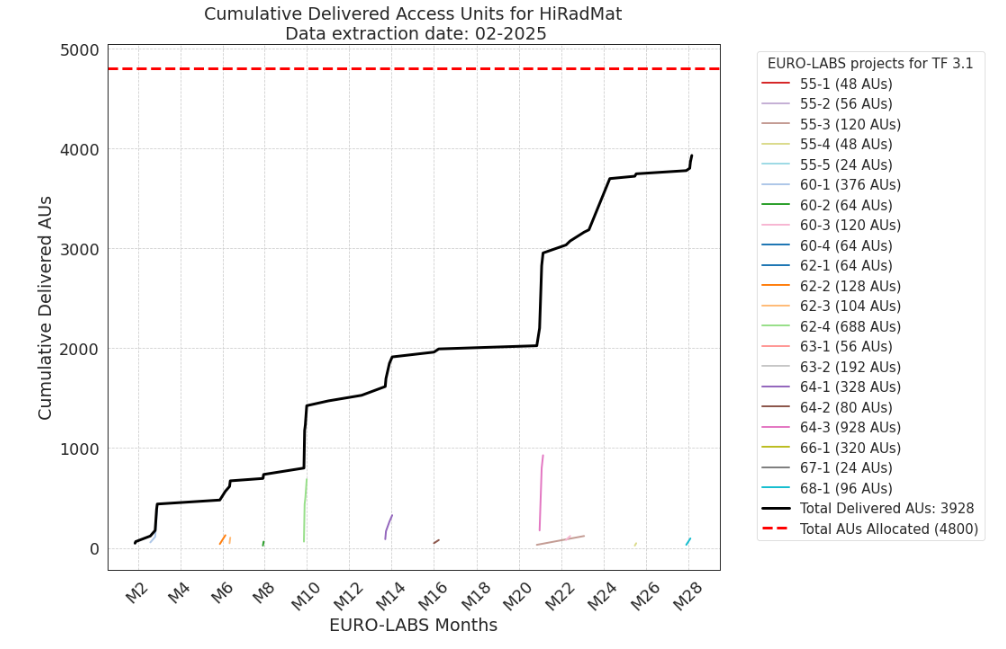
\includegraphics[width=0.48\linewidth]{graphics/overall_evolution_hiradmat.png}
    % \captionsetup{justification=centering}
    \caption{Access Units spent (left) and evolution in time (right) in HiRadMat to the end of P2.}
    \label{fig:wp3-hrmt-stat}
\end{figure}

% The evolution of the spent access units overall, and only for the RP2 is shown in Figures~\ref{fig:overall_evolution_hiradmat} and~\ref{fig:RP2_evolution_hiradmat}.
%\begin{figure}[!h]
%    \centering
%    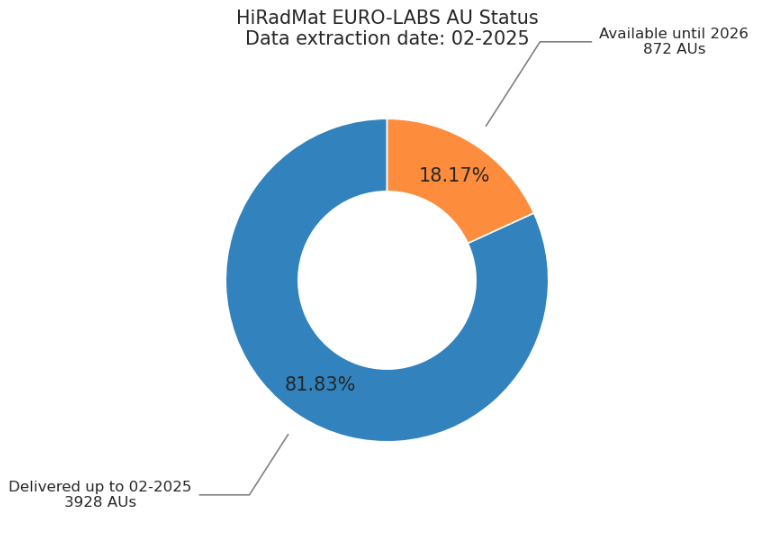
\includegraphics[width=0.75\linewidth]{graphics/stat_pie_hiradmat.png}
%    \caption{Access Units spent in HiRadMat in all reference periods. A total of 4800 AUs were allocated to the facility ; 3696 AUs have been already spent in this second reference period, and 232 AUs have been spent after September 2024 and until today (Feb. 2025). }
%    \label{fig:stat_pie_hiradmat}
%\end{figure}

Figure~\ref{fig:gender_distr_hiradmat} shows the gender and age distribution of the funded users in HiRadMat. 
\begin{figure}[!h]
    \centering
    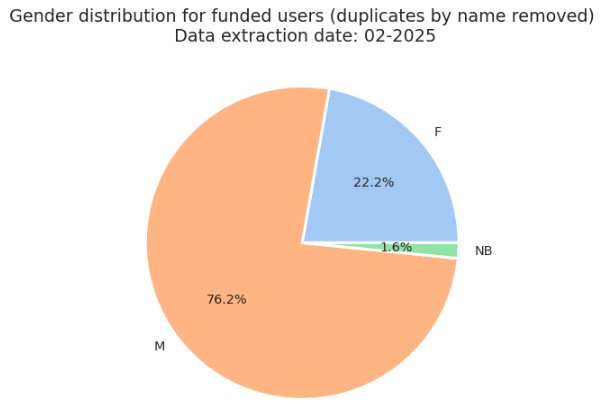
\includegraphics[width=0.48\linewidth]{graphics/gender_distr_hiradmat.png}
    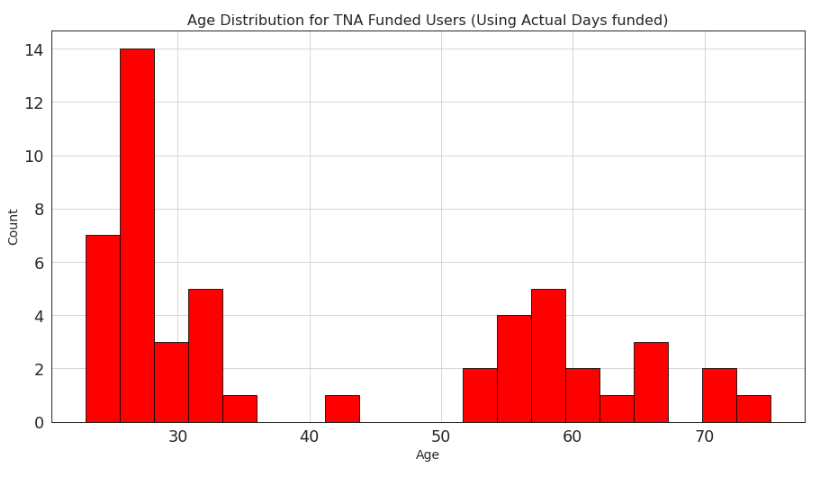
\includegraphics[width=0.48\linewidth]{graphics/age_distr_hiradmat.png}
    % \captionsetup{justification=centering}
    \caption{Gender(left) and age (right) distribution of TA funded users in HiRadMat.}
    \label{fig:gender_distr_hiradmat}
\end{figure}
The age distribution reflects the effort made within the USP to promote graduates and young researchers in the early stages of their careers. At the same time, the presence of senior researchers in the preparatory, data-taking and experimental phases is absolutely necessary for the success of the experiments and the transfer of knowledge. 

%For the funded users, the gender distribution is shown also in Figure~\ref{fig:gender_distr_hiradmat}, removing the duplicates by name. 
% is indicating that as per the instructions for TA, the user selection panel has approved mostly undergraduate and postgraduate students, at the early stages of their careers and fewer senior researchers (professors and tenured researchers). However, specifically at HiRadMat, the presence of the 
%The age distribution for the funded users is shown in Figure~\ref{fig:age_distr_hiradmat}.
%\begin{figure}[!h]
%    \centering
%    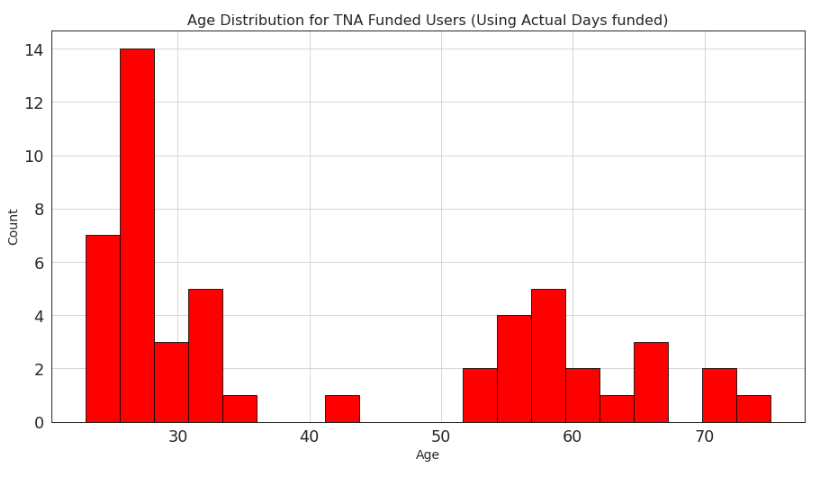
\includegraphics[width=0.75\linewidth]{graphics/age_distr_hiradmat.png}
%    \caption{Age distribution of funded users in Task 3.1 (HiRadMat). The majority of the supported users is at the early stages of their career, while a few senior researchers or recognized scientists at their field have been also necessary during the preparatory or the post-irradiation phases.}
%    \label{fig:age_distr_hiradmat}
%\end{figure}
%\begin{figure}[!h]
%    \centering
%    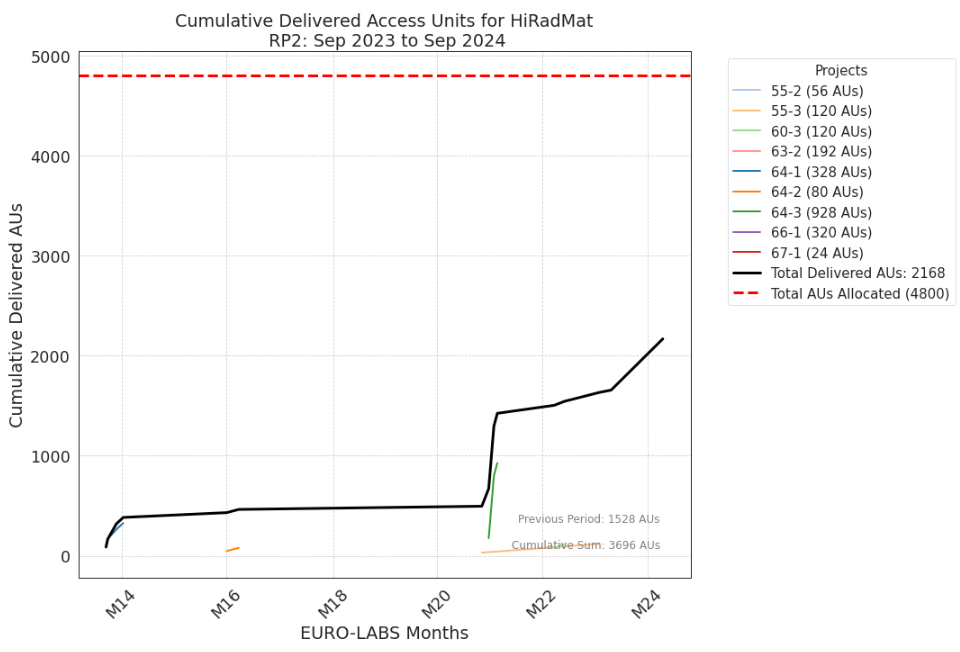
\includegraphics[width=0.9\linewidth]{graphics/RP2_evolution_hiradmat.png}
%    \caption{Evolution of delivered AUs for HiRadMat during the second reference period (RP2) and breakdown of AUs per project.}
%    \label{fig:RP2_evolution_hiradmat}
%\end{figure}

\subsubsection*{Main Results and Achievements}

HiRadMat continued to provide transnational access (TA) to several projects, supporting not only accelerator R\&D but also paving the way for novel uses of accelerator facilities in astroparticle research. 

The facility remains highly popular among users, thanks in part to targeted publicity efforts made through conferences and workshops, which have increased its visibility within the scientific community. Furthermore, the high motivation and expertise of the beam team combined with the strong local technical support, has played a critical role in helping users successfully complete their experiments and produce high-quality scientific results.

Highlights of the experimental results from the funded projects are presented in Section~\ref{sec:wp3_scientific_output}.

\paragraph{Progress in the service improvements tasks}

EURO-LABS is supporting a service improvement project for HiRadMat, focused on enhancing the calibration of the SPS Beam Position Monitor (BPM) system (designated "ALPS") in both the ring and the extraction line toward the facility. Accurate beam position measurements are particularly crucial for many experiments that require precision and repeatability beyond what is presently achievable.

As part of this effort, a neural network is being developed to improve the residual errors in the BPM device calibration, which is currently based on a simple polynomial fit. The task is complex and requires careful evaluation of the results, particularly because the performance of the existing calibration method had not previously been studied in such depth. Progress is well underway, led by a doctoral student at CERN in collaboration with the University of Oxford.

Preliminary results comparing the residuals produced by the neural network against those from the traditional polynomial fit — using the response from a single electrode of an ALPS Beam Position Monitor (BPM) — are shown in Figure~\ref{fig:wp3-hrm-si}. The newly developed neural network approach shows improved performance compared to the existing polynomial fit. Further optimization studies are ongoing, with the aim of minimizing beam position measurement errors.

\begin{figure}[!h]
    \centering
    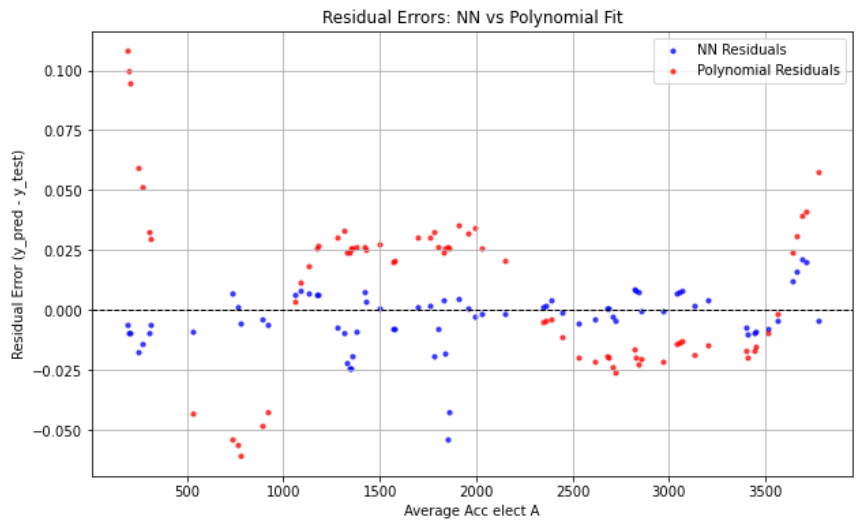
\includegraphics[width=0.75\linewidth]{graphics/hiradmat_SI.png}
    \caption{Residuals for the calibration curve of an ALPS Beam Position Monitor, based on the response of a single electrode.  (Courtesy of V. Stergiou and A. Boccardi, CERN).}
    \label{fig:wp3-hrm-si}
\end{figure}

The objective is to define and validate the algorithm for use within EURO-LABS. The implementation is planned to start in 2029, after the CERN long shutdown (2026-2029). This timeline provides sufficient time for the prototyping and testing of new electronic components, with the new system becoming operational after the restart.

\subparagraph{Task 3.2 : Technology Infrastructures} \mbox{}

This task includes six specialized facilities focused on accelerator component R\&D also connected to the AMICI~\footnote{\url{https://amici.ijclab.in2p3.fr/}} collaboration. The facilities remain in close contact with ongoing R\&D initiatives in EUROPE as the I.FAST project~\footnote{\url{https://ifast-project.eut}} but also world-wide as PIP-II~\footnote{\url{https://pip2.fnal.gov}}, where demand for tests of magnets and superconducting cavities could arise, in an effort to attract users. However already observed in P1, only three of these facilities have so far been able to support TA projects and deliver Access Units (AUs).

Technical works or upgrades initiated by the facilities' management to support long-term service contracts with large projects have reduced the availability of certain infrastructures for individual TA projects eligible for EURO-LABS funding. This is particularly the case for the INFN LASA and THOR facilities, as explained in more detail below. Additionally, the unexpected loss of local technical expertise, combined with difficulties in assigning replacements, has blocked the UU-FREIA facility from continuing to provide TA, despite its promising start during P1.

During the 18 months of P2, a total of 744 AUs were delivered, mainly through remote access, bringing the cumulative total since the beginning of EURO-LABS to 1,236 AUs. This corresponds to 30\% of the planned AUs if only considering operational facilities, or 10\% when considering all six facilities as initially foreseen in the Grant Agreement.

The WP and Task Leaders are closely monitoring the situation. There is optimism that, with the completion of technical works in 2025, some facilities will be able to resume the delivery of TA projects, with discussions already underway. In parallel, a mitigation plan has been prepared, which foresees a reshuffling of resources within the Task, and, if necessary, at the WP level.

Details per facility are provided in the following paragraphs.

% \todo{Briefly explain the progress of the task in context to the DoA.}

\subsubsection*{Main Results and Achievements}

% \todo{Briefly summarise the main results and achievements of the WP in context of the DoA.}

\subparagraph{UU-FREIA}

FREIA had a spectacular startup during P1, delivering 50\% of the AUs promised in the Grant Agreement. However, during P2, FREIA has not provided any transnational access (TA). Although there were preliminary discussions about testing a PIP-II cavity, unfortunately no follow-up actions materialized.

A key limiting factor is the facility’s availability for small, short-term TA projects, given its current engagement in large-scale, long-term contracts for series testing of production modules destined for major future accelerator installations in Europe. This series testing significantly restricts the use of the liquefier, a critical component for carrying out short-term experimental work. In addition, the facility experienced the departure of a key mechanical engineer — an expert in cryogenics with deep knowledge of the installation — without a rapid replacement, further complicating the planning of future tests.

Nevertheless, all efforts will continue to be made to support any future TA requests should they arise.


\todo{I am waiting a summary fro Rocio on the status of the service improvements}

%To answer your questions/s: yes, they are interested in using our facility and will sign the document (it’s already done by our side), but you know how it is with especially MYRRHA, we are requested to not give any information (let it be slides, or just in a general chat) if it has not been previously approved by them. And even more without a signed contract…So unfortunately this is not just because we do not have yet have a signed contract, this will always be the case: they being mention in any way in future slides will need to be sent for their approval.
 

% I write you because we are in initial discussions with FNAL about the possibility of testing a PIPII cavity in Gersemi, and I have a question that I forgot the answer to after the SAM…Provided the TA is granted by the committee, the total amount of units that FREIA can provide, is it the 20\% of the total? For example, FREIA has a total of 960 TA units, could we then only provide max 192 TA units for this test? So could they then pay the rest of the amount themselves if needed?

% Since we do not know how is it going to look in the future for us (since we will have the liquefier kind of blocked by Minerva testing, with some small slots here and there, maybe) we would like to have this test done and accounted, even though it is not from an European Institution.

\subparagraph{INFN-LASA} 

LASA (Laboratory for Accelerators and Applied Superconductivity) hosts four test facilities dedicated to: superconducting (SC) magnets, superconducting (SC) RF cavities, high-brightness photocathodes for electron sources, and laser applications to high-power Fabry–Perot cavities and advanced timing systems. These facilities were initially conceived to support LASA’s internal research activities.

So far, LASA has not been able to accept any transnational access (TA) projects. The transition of these facilities towards external user access progressed more slowly than initially anticipated during 2023, due to two main factors. First, a significant portion of the researchers and the already limited technical support staff were heavily involved in planning the expansion of LASA’s infrastructure, which is set to double the laboratory’s surface area. Second, the gradual conversion and upgrading of critical infrastructures — including electrical systems and the cooling systems for cavities and magnets — toward the new layout and future installations blocked the availability for external users.

According to the current planning, these upgrade activities of LASA are expected to be completed in 2025. If this timeline is met, it would leave sufficient time to consider few TA requests until the project ends in 2026 from the pool of users who had already expressed interest in 2023, assuming their interest remains active.

% LASA (Laboratory for Accelerators and Applied Superconductivity) is characterized by the presence of four test facilities devoted to: Superconducting (SC) Magnets, Superconducting (SC) RF Cavities, High Brightness Photocathodes for Electron Sources and Laser Applications to High Power Fabry Perot Cavities and Advanced Timing Systems. The four facilities have been conceived as facilities to support the research activities undergoing at LASA.

%So far LASA was not able to accept any TA project. This because the activities relating to a transition of these facilities towards use by external users slowed down during 2023 compared to the initial expectations for two reasons: first, the commitment of a relevant part of the researchers involved and of the technical support (the latter already quite limited) of the laboratory in relation to the planning of the expansion of the LASA (by a factor equal to approximately 100\% of the surface), and second the gradual conversion of the current infrastructures relating to the electrical systems and the cavity and magnet cooling system towards the new layout and future installations.

% In the present planning these activities should be completed in 2025, which if indeed the case, leaves time to consider TA requests among the few who expressed interest already in 2023, should their interest remains. 

% Once these activities have been completed, we are now able to prepare the forwarding of requests discussed and received in the meantime in relation to some specific activities.
%Of course due to the specific period of the year we have to discuss the confirmation for these previous requests. 

%Superconducting cavities: we discussed a request from researchers from DESY and CEA for the test of a prototype SC RF cavity for the PIP II project. The test will last a week considering 3 days for cooling down and one for warming up. The measurement process will last 2 days (for a total of nearly 12 hours/each day to save on liquid helium). Looking at the relatively short time dedicated to the measurements we are evaluating the possibility to operate in a remote fashion.
%The same opportunity for a separate test with longer measurements time involved will be used by a researcher from JLab to learn as much as possible on handling SC RF cavities for an ERL Linac of mutual interest. For this request we have to consider also some issue related to the availability of the requested volume of liquid helium (1500 liters) with so a short forewarning.

%Laser applications: a request has been discussed about a user from IJCLab and University of Orsay to carry out measurements on the laser system available at LASA for photocathode and Fabry Perot cavity. He plans to stay here a week (5 days) working 8-10 hours every day. This would be the first activity of a longer usage of our facility.

%High Brightness Photocathodes: a request has been recently issued to make some tests on a HV DC test stand related to the development of a DC Gun to investigate the behavior of specific materials handling High Voltage. The request come from the University of Uppsala. This request would be the first of a few, involving also tests with materials at cryogenic temperature.


\subparagraph{INFN-THOR}

The THOR (Test in Horizontal) facility in Salerno is focused on superconducting magnet systems testing. Equipped with advanced cryogenic, vacuum, and electrical testing setups, the facility ensures high-quality assessments of critical technologies in the field of superconductivity. 

However up to June 2024 the Facility was fully engaged in supporting the development and testing of accelerator components, particularly for the GSI/FAIR project. Specifically, a series of tests on the SIS100 quadrupole doublet modules for the test facility FAIR have been performed for the final acceptance before their installation in the SIS100 tunnel now under construction in Darmstadt. Given the tight timeline of the test plan, the allocated time for Transnational Access (TA) was so far limited. This constraint was primarily due to the high-priority testing schedule, which required significant resources and time allocation.

Starting from July 2024, access to the THOR facility has been restricted due to an ongoing upgrade and consolidation. This upgrade aims to enhance the facility’s capabilities, improving efficiency and increasing the throughput of testing activities. Consequently, no external access could be scheduled during this period and until February 2025.

By March 2025, the commissioning of a fully equipped test facility will start, providing testing opportunities for TA users in the field of cryogenic, vacuum, electronics. However the continous engagement of the Facility management to support the GSI/FAIR project as high-priority poses potential constraints on planning TA access. All efforts will be made to accommodate possible external access slots, should the interest arises. 

\subparagraph{SUPRATECH}

The facility is actively participating in the PIP-II project of FermiLab in USA achieving through RAs to perform the tests and full validation of SC cavities designed within the project. The SUPRATECH maintains strong links with the CEA/LRFU Sygergium facilities, offering combined tests of accelerator components for full validation. 

Among its users, SUPRATECH is actively involved in the PIP-II project at Fermilab in the USA, performing tests and full validation of superconducting (SC) cavities designed for the project. SUPRATECH maintains strong collaborative ties with the CEA/LRFU Sygergium facilities, offering combined testing of accelerator components to ensure full validation.

% Three projects during the reference period. 

%For Zanon company (Italy) : Testing at cryogenic temperature of 3 prototypes Spoke resonator (SSR2) for PIP2 project
%All three cavities tested and shipped to Fermilab
%2 cavities have been validated and reached PIP-II project specifications
%1 not validated but shipped to Fermilab for R\&D tests
%Testing report issued to Zanon company.
%For Fermilab (USA) : 2 cryogenic tests of 1 prototype Spoke resonator (SSR1) before/after plasma processing.
%Under validation by USP

\subparagraph{Synergium}\mbox{}

\todo{Need input from Sylvie}

\subparagraph{XBOX}

The XBOX facility hosts klystron-based X-band test stands located at CERN. These test stands are dedicated to the testing and development of high-gradient accelerating structures and high-power RF components, initially developed for the CLIC project, but also applicable to R\&D for X-band FELs, Compton/Thomson sources, and potential RF units for linear accelerators. As a result, XBOX offers unique, state-of-the-art yet highly specialized capabilities, which makes it challenging to meet a broader and more diverse needs of a wider external user community.

Despite sustained publicity efforts during the reference period, the XBOX facility did not attract any new transnational access (TA) projects. 

\subparagraph{Task 3.3 : Electron and Plasma Beams} \mbox{}

% \todo{Briefly explain the progress of the task in context to the DoA.}

This task includes six facilities located across three laboratories, offering access to electron or plasma beams.

A combination of technical, safety, and administrative issues has prevented three of the facilities from becoming operational and providing access units since the beginning of EURO-LABS. The fourth facility, is a state-of-the-art plasma beam installation, which is currently being upgraded, thus not yet easily accessible to external users. The remaining two facilities were fully active in P2 and have performed exceptionally well, delivering 65\% more AUs than expected for the 18-month period of P2, raising the cumulative total to 1490 AUs since the start of the project. This figure for the two facilities, represents 34\% more AUs than originally promised at this stage, demonstrating their strong potential to absorb additional TA requests and potentially compensate for the lack of access at other facilities.

Beyond the TA projects, good progress has also been made on the Service Improvements, with the projects entering their implementation phase as planned.

Details for each facility are provided in the following paragraphs

\subsubsection*{Main Results and Achievements}

%\todo{Briefly summarise the main results and achievements of the WP in context of the DoA.}

\subparagraph{INFN-LNF}

The Frascati National Labs (LNF) of the Italian Institute for Nuclear Physics (INFN) offers TA through 2 facilities: BTF (Beam Test Facility) and SPARCLAB (Sources for Plasma Accelerators and Radiation Compton with Laser And Beam).

BTF is an infrastructure mainly dedicated to the development and testing of particle detectors, providing primary, fixed energy beam and secondary electron or positron beams with continuously tunable energy from \SI{30}{\MeV} to \SI{780}{\MeV} and multiplicity from $10^{10}$ particles/pulse down to a single particle/pulse in a Poisson stochastic regime.
SPARCLAB is a research infrastructure based on the combination of the high-brightness SPARC photo injector, providing electron beam at energies up to \SI{180}{\MeV}, with the high intensity FLAME laser, able to generate infrared laser pulses with $10^{19}$~W/cm$^2$ intensity. The facility is generally devoted to the R\&D on novel acceleration techniques, advanced diagnostics and generation of radiation ranging from THz to extreme UV light. 

In the reporting period both facilities have been in operation apart from some maintenance periods and, mostly for SPARCLAB, upgrade and installation activities.

\subparagraph{INFN-LNF/BTF}

The operation of BTF in the reporting period has been quite smooth and regular. According to its specific inclination, the facility run for a wide user community in terms of research fields and geographical distribution (national and international). In this context the implementation of the TA modality supported by EUROLABS resulted to be almost straightforward. In the reporting period the facility provided access to 3 EUROLABS supported experiments, for a total of 4 weeks of run delivering 672 AUs, corresponding to 57\% of the promised total in the GA. 

Highlights of the experiments in Section~\ref{sec:wp3_scientific_output}

\subparagraph{INFN-LNF/SPARCLAB}

The operation of SPARCLAB in the reporting period was limited because of a total of 6 months of shutdown necessary to install a consolidation/upgrade plan and for setting-up a new facility for FEL radiation production in the THz range, the SABINA project. This program was partially funded by the local Regional Government and its timeline was mandatory and could not be postponed. SPARCLAB is also the test-stand were the R\&D on plasma acceleration, which is the backbone of the laboratory flagship project EuPRAXIA, is being carried on with the highest priority. The combination of these 2 circumstances, i.e. the installation of the new facility and the high priority assigned to internal scientific program during the operation period, left essentially no-space to accommodate slots for TA. As a consequence, no TA have been provided by SPARCLAB in the reporting period

% \separatorline{0.3em}{0.5\textwidth}{0.4pt}

\subparagraph{KIT-FLUTE} FLUTE delivered so far no TA experiment, however several important and fundamental improvements have been made to this accelerator test facility. During the evaluation of the EURO-LABS TA proposal preparatory FLUTE experiments showed that the shot-to-shot stability, especially the pointing stability, was not sufficient for more advanced experiments. We traced this back to the low stability of the aging RF system. KIT therefore decided to completely refurbish the entire RF system. We installed a new photoinjector electron source from RadiaBeam, a new linear accelerator (linac) module from Research Instruments. We also used this occasion to install two separate RF sources and amplifiers from ScandiNova for the photoinjector and for the linac module. This renewal now allows a more precise and, above all, independent setting of parameters (energy, phase) for the photoinjector and the linac, respectively. Furthermore, we replaced the photoinjector laser system with a new and more powerful one permitting a wider range of experiments like, for instance, FLUTE experiments with split-ring resonators, that were requested by users in the past for Transnational Access.

These necessary refurbishments of almost all fundamental components of the accelerator led unfortunately to some delays for restarting FLUTE. This was mostly due to problems with the two new klystrons, requiring several service visits by the manufacturer. After solving these issues, we could show during commissioning of the new RF system an improved stability by a factor of 10.

After finalizing the commissioning of the linac and the bunch compressor, as well as the associated diagnostics sections with the new RF system, we are now ready to perform first TA experiments with the completely refurbished accelerator. 
Spring 2026 we will have to dismantle FLUTE temporarily as scheduled to be able to install the novel cSTART test accelerator facility at KIT, a new storage ring in the FLUTE experimental hall. This new installation will also include a laser plasma accelerator. In parallel FLUTE will be installed again and connected to the cSTART ring, where FLUTE serves as an injector to cSTART or an independent test facility.

\subparagraph{KIT-KARA}

KARA provided TA for 5 experiments during the reference period, delivering 598 AUs, which combined the the AUs offered in P1 make the total 818 AUs corresponding to 93\% of the total promised at the GA. 

Highlights of the experiments in Section~\ref{sec:wp3_scientific_output}

On the \textbf{Service Improvements:}

\underline{\em{Simulation and Measurement Framework activities}}:  
The frame work online optics simulation in ocelot was extended by scripts to measure automated different accelerator parameters like chromaticity, dispersion, beta function and response matrix. Further tools for different beam bases alignment  techniques are currently in development together with one TA activity. Another class of measurements are camera image processing. There different open source tools and analysis frameworks have been evaluated. It was decided to use the area Detecot {Ref: \url{https://areadetector.github.io/areaDetector/index.html} for this application which is currently implemented at KARA and FLUTE. KIT also joined the python accelerator middle layer activities (Ref:\url{https://github.com/python-accelerator-middle-layer}) to benefit from the shared effort. The next step is to contribute to the code development and deployment of the system at KARA and FLUTE.

\underline{\em{Data Management Framework Activities}}: 
In-depth analysis and comparison of three research data management platforms: B2Share~\footnote{https://b2share.eudat.eu/}, RADAR~\footnote{https://radar.products.fiz-karlsruhe.de/en}, and Kadi4Mat~\footnote{https://kadi.iam.kit.edu/}. This evaluation aimed to select suitable tools for managing experimental physics data effectively. Each platform was assessed based on its capabilities for data storage, accessibility, and metadata handling. Special attention was given to the ability to structure and retrieve metadata efficiently. Analyzing different experiments revealed that the metadata must be identified at an individual measurement level. This ensures precise documentation and supports reproducibility in research workflows. A flexible metadata generation schema is under preparation to accommodate diverse experimental requirements. The evaluation also considered automation possibilities to reduce manual metadata entry. Security, scalability, and integration with existing infrastructure were additional factors in the assessment. The final selection will balance usability and long-term sustainability for research environments.

Next steps: Based on the gained experience, select the most suitable tool and implement the Data Handling Framework and metadata generation. Validate the chosen solution in real-world scenarios and refine the approach based on feedback.

% \separatorline{0.3em}{0.5\textwidth}{0.4pt}

\subparagraph{CLARA}
 
During the reporting period, the CLARA facility has continued its reconfiguration to enable operation at \SI{250}{MeV}. 
In parallel, the full energy beam exploitation (FEBE) experimental hutch has been assembled and major sub-assemblies such as the user experiment chambers, magnetics and light boxes have been installed. The FEBE Ti:sapphire laser system has also been commissioned, allowing the synchronised interaction of electron bunches with an approximate \SI{100}{TW} laser. 

As of March 2025, the CLARA build phase is complete and the electron gun has been successfully tested. Due to the extensive redevelopment of CLARA and delays to the operational reinstatement of the facility, the facility has not delivered any TA projects during the period. However, sub-system recommissioning and beam threading will continue through summer 2025 and it is anticipated that user beam access, including TA projects, will restart in Q3/Q4 2025.

% \separatorline{0.3em}{0.5\textwidth}{0.4pt}

\subparagraph{LPA UHI100 (CEA-LIDYL} 

No beamtime was delivered during P2 (and similarly during P1) due to delays caused by the French Nuclear Safety Authority (ASN) in granting a license for operating the facility. We are still awaiting the final operating license from ASN/CEA.

The entire experimental setup, including the laser and experimental equipment, was relocated from the main CEA site at Saclay to a satellite facility at Orme des Merisiers, just a few kilometers away. In order to begin full laser energy operations and deliver the laser-driven electron source, we were required to obtain a license from ASN (Nuclear Safety Authority). A temporary license was issued at the beginning of 2024, valid through the end of August 2024, which limited the generating conditions to a maximum electron energy of \SI{50}{MeV}, a repetition rate of one shot per minute, and a maximum charge of \SI{15}{\pico C/bunch}, thus resulting in degraded operating conditions.

A visit by ASN was scheduled on July 3rd, 2024, to assess the operating conditions of the laboratory. Based on the feedback received during the visit, modifications were suggested, and a revised request for experimental parameters aligned with our scientific program (higher energy, repetition rate, and charge in the electron beams) was submitted.

At the end of December 2024, ASN granted CEA a temporary license for communication with our team scheduled on January 13th, 2025. This license is valid for one year and permits parameters of 200 MeV, a maximum repetition rate of \SI{0.3}{Hz}, and a maximum charge of \SI{300}{\pico C/bunch}.

Before proceeding with full-power operations on target, we need to conduct test experiments to verify the deposited dose by the electrons and check the consistency of simulations with the experiments. These tests are planned for March 2025, and if all conditions are met and consistent, we should be able to move forward with full-power operations on target.

\todo{Text to include here from Sandrine on Service Improvement}

\subparagraph{Task 3.4 : Applications} \mbox{}

% \todo{Briefly explain the progress of the task in context to the DoA.}

This task includes two facilities: the {\bf INCT/RAPID} and the {\bf CERN/CLEAR}. During the reference period both facilities were able to provide 11 TA projects, delivering 385 AUs raising the total to 643 AUs corresponding to 36\% of the promised AUs in the GA. 

Details are briefly described below. 

\subsubsection*{Main Results and Achievements}

% \todo{Briefly summarise the main results and achievements of the WP in context of the DoA.}

\subparagraph*{INCT RAPID} 
During P2, the INCT RAPID facility provided access with EURO-LABS support, conducting seven projects (one of which is still ongoing) delivering 105 AUs. The experiments utilized the following instruments:
\begin{itemize}
\item LAE 10 accelerator with nanosecond pulse radiolysis setup – used to investigate basic mechanisms of ionizing radiation interactions in biological systems.
\item Electronica accelerator, generating a beam of electrons with an energy of 10 MeV – for sterilization and materials modification.
\item ILU 6 accelerator, utilizing an electron beam with energies of 1.7 MeV and < 300 keV – for controlled depth of electron range in treated products.
\end{itemize}
For the experiments carried out at the RAPID infrastructure, dosimetry measurements were performed by the INCT Laboratory of Technological Dose Measurements to ensure precise and accurate dose delivery to the treated samples. Additionally, other INCT infrastructure, such as Electron Paramagnetic Spectroscopy, was used to help characterize radiation-induced effects in materials.

The experiments focused on the application of electron beams to investigate the mechanisms of radical interactions, radiation-induced effects in materials, and the effects of electron beam irradiation on food and food ingredients. In the upcoming year, plans are in place to adjust the experimental setup for irradiation in the gaseous phase, in response to newly received project requests. This modification will broaden the scope of research conducted at INCT within the EURO-LABS framework.

Highlights of the TA experiments are listed in Section~\ref{sec:wp3_scientific_output}

% \separatorline{0.3em}{0.5\textwidth}{0.4pt}

\subparagraph*{CERN-CLEAR Facility}

CLEAR was fully operational during the reference period able to provide TA to four experiments delivering 280 AUs, which cumulative to those delivered in P1 raise to a total of 448 AUs correspond to 37\% of the total promised at the GA. 
The facility is heavily used for conducting research on future electron accelerators, in parallel to a rigorous research program on FLASH radiotherapy. 

Highlights of the TA experiments are listed in Section~\ref{sec:wp3_scientific_output}

On the \textbf{Service Improvements:}
The CLEAR planned service improvements are meant to improve the quality of the measurements and of the data acquisition process in areas critical for a large part of the users and increase the number of users that can access the facility per unit time. 
\begin{figure}[H]
    \centering
    % 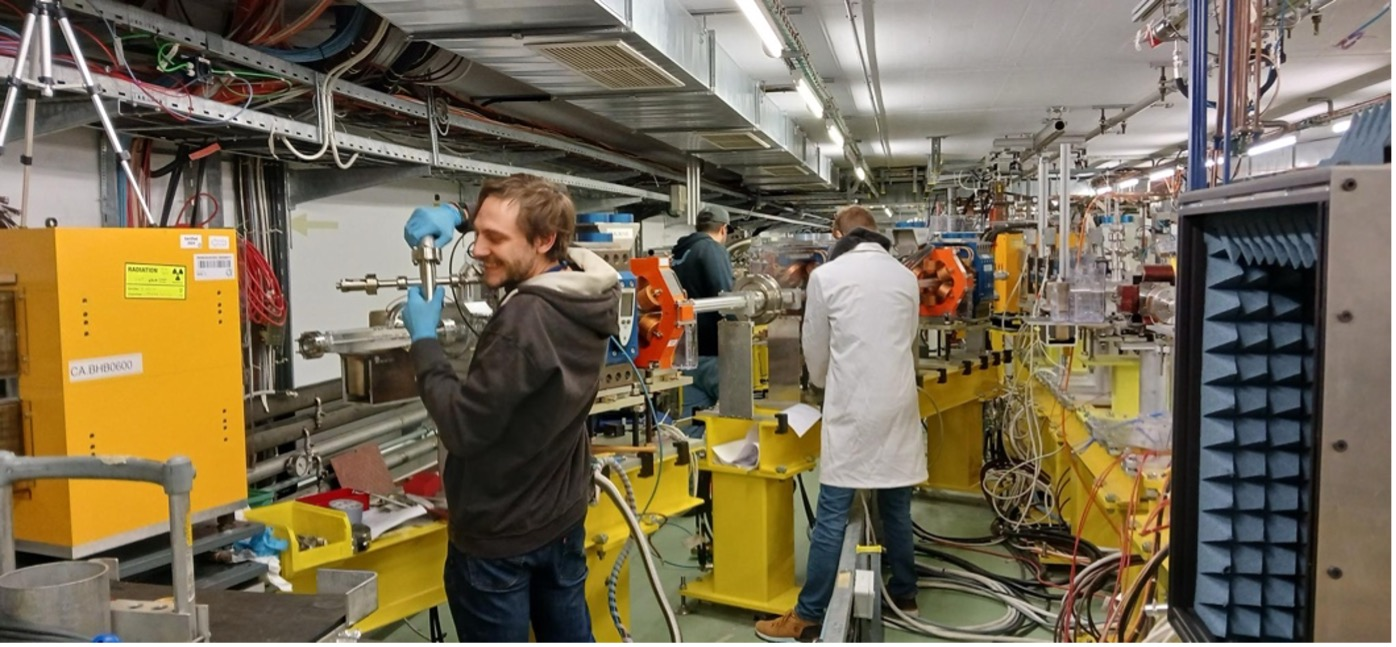
\includegraphics[width=0.78\linewidth]{graphics/CLEAR-2ndBLinstallation.jpg} \\
    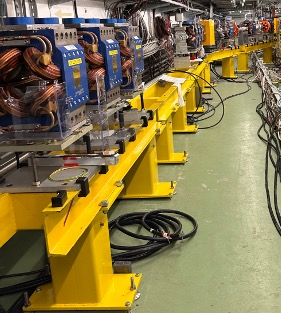
\includegraphics[width=0.60\linewidth]{graphics/CLEAR-2ndBLJan25.jpg}
    \caption{%Top: photo during the installation of the new beam line in the CLEAR facility.
    Photo of the new beam line of the CLEAR facility at the end of installation activities in January 2025.}
    \label{fig:wp3-clear-2ndbl-inst}
\end{figure}

The main CLEAR service improvement consist in the construction of a new beam line. This line will allow a faster turn-around of experiment, minimizing installation time, and will provide an end-of-line experimental station with added beam flexibility and improved handling/measurement hardware. The activity has been fully approved by CERN management in June 2023 and the beam line design was completed at beginning 2024. Most of hardware is being re-used from the previous CTF3 installation. Most components of the beam line have been installed in the winter shut-down 2024-2025 (see Figure~\ref{fig:wp3-clear-2ndbl-inst}).

The completion of the installation and its initial commissioning is planned for August-September 2025. Although mainly funded by CERN/CLEAR budget (total estimated cost ~ 180 kCHF), several items, in particular ones relevant for the end-of-line experimental area, have been purchased using EURO-LABS funding. These includes a beam current measurement device (ICT), an optical table, vacuum and optical components, beam screens and associated cameras, plus drawing office work. A new version of the handling C-robot was also designed, built and tested. Additional items still to be purchased using EURO-LABS funds are 1) an ionization chamber for real-time dosimetry, 2) two vacuum chambers for the two new beam line dipoles, 3) some ADC and timing modules and other acquisition and data handling hardware.
%\begin{figure}[H]
%    \centering
%    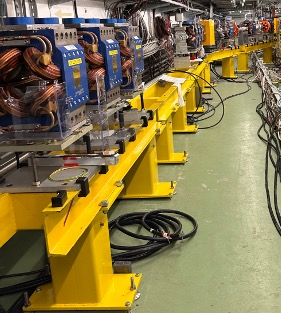
\includegraphics[width=0.78\linewidth]{graphics/CLEAR-2ndBLJan25.jpg}
%    \caption{Photo of the new beam line of the CLEAR facility at the end of January 2025.}
%    \label{fig:wp3-clear-2ndbl}
%\end{figure}

\subsubsection*{Deviations and Corrective Actions}

% \todo{Briefly summarize any deviations and performed corrective actions of the WP in context of the DoA.}

The WP3 facilities are currently lagging behind in providing the required number of TA projects and Access Units (AUs). By the end of P2, the facilities have collectively delivered only 26\% of the promised TA projects and 35\% of the planned AUs. However, behind this overall picture, there are significant variations between individual facilities as explained above.

To address these deviations, we will continue to closely monitor the situation and propose adjustments to the allocation of project resources. Priority will be given to reallocating resources towards higher-performing facilities, first within the Task and, if necessary, across the entire Work Package. This strategy aims to maximize the overall TA delivery by supporting additional projects at facilities with greater TA capacity.

Based on present performance and future expectations we can classify the facilities as follows:
\begin{description}
    \item[Overperforming:] HiRadMAt, KIT/KARA. \\
        Performing very well. Could absorb additional TA projects if needed.
    \item[Within expectations:] LRFU-Synergium, IJCLAB-SUPRATECH, CEA-LPA-UHI100, STFC-CLARA, INFN-BTF, INCT-RAPID \\
        Maintaining expected performance levels. Expected to deliver according to the original schedule. 
    \item[Below expectations:] UU-FREIA, INF-LASA, INFN-THOR, XBOX, KIT/FLUTE, INFN-SPARCLAB, CLEAR. \\
        Facing technical or administrative delays. Unlikely to fully deliver the planned TAs. Accepted to release TA resources.
\end{description}
Further details provided for selected facilities in the following paragraphs.

% Table~\ref{tabl:wp3-deviations} summarizes the current status, with further details provided for selected facilities in the following sections.
%\begin{table}[H]
%    \centering
%    \begin{tabularx}{\textwidth}{|c|X|} \hline
%    \rowcolor{lightgray}
%    \textbf{Facility} & \textbf{Comments} \\ \hline
%    \multicolumn{2}{|c|}{\textbf{Overperforming}} \\ \hline
%    HiRadMat & \multirow{2}{\hsize}{Performing very well. Could absorb additional TA projects if needed.} \\ 
%    KIT/KARA & \\ \hline
%   \multicolumn{2}{|c|}{\textbf{Within expectations}} \\ \hline
%    LRFU-Synergium & \multirow{6}{\hsize}{Expected to deliver according to the original schedule. Maintaining expected performance levels.} \\ 
%    CEA-LPA-UHI100 & \\ 
%    STFC-CLARA & \\
%    INFN-BTF & \\
%    IJClab-SUPRATECH & \\
%    INCT-RAPID & \\ \hline
    
%   \multicolumn{2}{|c|}{\textbf{Below expectations}} \\ \hline
%   UU-FREIA & \multirow{6}{\hsize}{Facing technical or administrative delays. Unlikely to fully deliver the planned TAs. Accepted to release TA resources.} \\ 
%   KIT-FLUTE & \\
%    XBOX & \\ 
%    INFN-LASA & \\
%    INFN-THOR & \\
%    INFN-SPARCLAB
%    CLEAR & \\ \hline
    
%    \end{tabularx}
%    \caption{Summary of WP3 facility status and group comments.}
%    \label{tabl:wp3-deviations}
%\end{table}

\paragraph{HiRadMat} HiRadMat has already used 82\% of its allocated 4800 Access Units (AUs) at the end of the second reference period. This high usage rate reflects the facility’s strong visibility, supported both by EURO-LABS dissemination efforts and the production of promotional videos. The remaining AUs are sufficient to cover part of the experiments planned for 2025; however, there will be no budget available to support the remaining 2025 experiments or those anticipated in 2026, the exact number of which is still uncertain.

HiRadMat would welcome additional funding to support continued transnational access, as well as user assistance with logistics and simulation efforts.

\paragraph{LPA UHI100 (CEA-LIDYL)} We have plan to deliver beamtime as much as we will be able to do. We have already a proposal from an Italian Team that should be submitted. The LPA-UHI100 facility team is considering the technical feasibility of the proposal with the applicants, before submission. And we are working on a 2nd proposal which could be the following of the 1st one, depending on the results obtained. We will keep advertising about the TNA through EUROLABS, participating to international/national conferences this year 2025.  We have already discussed with other communities and in particular physico –chemists and radiobiologists who want to use the extrem dose rate delivered by our laser-driven electron sources to test the response of biological material to such irradiations, in the context of FLASH radiotherapy, and to validate dosimeters developed for such high dose rate source.  

1 beam time project (160 hours) for 2025, in preparation for submission next march 2025, to test a temporal diagnostic adapted to the extremely short duration of the LPA electron beams. The beamtime could be allocated at the second semester of 2025.

We will try to deliver another beamtime period (160hours) in the first semester 2026, planning a maximum of 2 runs in 2026 (320hours max in 2026).

\paragraph{INFN-LNF/(BTF, SPARCLAB)}

The perspectives for the completion of the EURO-LABS TA program for BTF look quite secure. The facility staff is now systematically promoting the opportunity of supported TA to the reference community, with positive returns, and 4 out of 7 TA weeks planned for the whole project have been already delivered. The staff is confident that the remaining 3 will be assigned and delivered by the end of 2025, and some space will be available to eventually accommodate 2-3 extra weeks in the 2026 before the project conclusion.
For what concerns SPARCLAB the situation looks far less optimal. As mentioned, none of the 9 weeks of TA allocated in the project have been delivered so far, and it not realistic to think recovering all in the time left till the end of the project for the mentioned reasons. In 2025 the new facility EuAPS funded by the Next Generation EU program will be installed in the SPARCLAB bunker requiring a 4 months shutdown. In the present scenario the number of allocable TA weeks at SPARCLAB before the EURO-LABS project end in August 2026 is 2-3. The SPARCLAB staff is committed to promoting this opportunity to its international reference community.

\subsubsection*{Milestones and Deliverables}

%{\fontsize{9}{11}\selectfont
%\begin{center}
%  \begin{tabular}[t]{!{\color{mygray}\vrule}p{0.10\linewidth}!
%  {\color{mygray}\vrule}p{0.60\linewidth}!
%  {\color{mygray}\vrule}p{0.20\linewidth}!{\color{mygray}\vrule} } \hline
%    \rowcolor{mycyan} & {\bf Title} & {\bf Status} \\ \hline
%    \cellcolor{mycyan}{\bf D1.x}: &  &  \\ \hline
%  \end{tabular}
%\end{center}
%}

There were no Milestones nor Deliverables for WP3 for the reference period. 

\subsubsection*{Project Meetings}


\begin{table}[H]
    \centering
    \begin{tabularx}{\textwidth}{|c|c|X|} \hline
        \rowcolor{mycyan}
        \textbf{Date} & \textbf{Meeting} & \textbf{Subject} \\ \hline
        2023-09-11 & TL02 - Task Leader's meeting & Regular meeting - progress report \\ \hline
        2023-09-20 & USP03- Task 3.1 & Evaluation Task 3.1 proposals \\ \hline
        2023-09-25 & WP3-03 Meeting & Regular WP meeting - progress report from the facilities \\ \hline
        2023-10-11 & Special meeting LASA-THOR & Discuss status and TA possibilities \\ \hline
        2023-10-23 & USP02- Task 3.4 & Evaluation Task 3.4 proposals \\ \hline
        2023-11-08 & USP02 Task 3.2 & Evaluation Task 3.2 proposals \\ \hline
        2023-11-16 & USP04 Task 3.3 & Evaluation Task 3.3 proposals \\ \hline
        2024-01-25 & WP3-04 Meeting & Regular WP meeting - progress report from the facilities \\ \hline
        2024-02-01 & USP04- Task 3.1 & Evaluation Task 3.1 proposals \\ \hline
        2024-03-18 & USP03 Task 3.4 & Evaluation Task 3.4 proposals \\ \hline
        2024-04-11 & USP04 Task 3.2 & Evaluation Task 3.3 proposals \\ \hline
        2024-09-06 & TL03 - Task Leader's meeting & Regular meeting - progress report \\ \hline
        2024-09-13 & WP3-05 Meeting & Regular WP meeting - progress report from the facilities \\ \hline
        2024-09-16 & USP-03 Task 3.2 & Evaluation Task 3.2 proposals  \\ \hline
        2024-10-29 & WP3-06 Meeting & Regular WP meeting - progress report from the facilities \\ \hline
        2024-11-06 & USP04- Task 3.4 & Evaluation Task 3.4 proposals \\ \hline
        2024-11-18 & USP05- Task 3.2 & Evaluation Task 3.2 proposals \\ \hline
        2024-12-04 & USP05- Task 3.1 & Evaluation Task 3.1 proposals \\ \hline
        2025-02-11 & TL04 - Task Leader's meeting & Regular meeting - progress report \\ \hline
    \end{tabularx}
    \caption{Summary of WP3 meetings and discussed subjects.}
    \label{tab:meetings}
\end{table}
%  {\color{mygray}\vrule}p{0.40\linewidth}!

%%%%%%%%%%%%%%%%%%%%%%%%%%%%%%%%%%%%%%%%%
%%%%%%%%%%%%%%%%%%%%%%%%%%%%%%%%%%%%%%%%%
%%% WP01
%%%%%%%%%%%%%%%%%%%%%%%%%%%%%%%%%%%%%%%%%

\tsubsubsection{WP4 - Access to RI for Detectors}

%%%%%%%%%%%%%%%%%%%%%%%%%%%%%%%%%%%%%%%%%
%%% Section content, please change!
%%%%%%%%%%%%%%%%%%%%%%%%%%%%%%%%%%%%%%%%%

\subsubsection*{Overview and Goals}

\begin{table}[H]
    \renewcommand{\arraystretch}{1.50}		
    \footnotesize   
    \begin{tabular}{*{3}{|p{0.10\textwidth}}|l|}
        \hline
        \rowcolor{mygray} \multicolumn{4}{|c|}{\textit{\color{white}Work Package Summary}} \\
        \hline
        \rowcolor{mylightergray} \textit{WP No.} & \cellcolor{white} 4 & \textit{Title of WP} & \cellcolor{white}  (TA3): Access to Research Infrastructures for Detector R\&D \\
        \hline
        \rowcolor{mylightergray} \textit{Start} & \cellcolor{white} M1 & \textit{End} & \cellcolor{white} M48 \\
        \hline
        \rowcolor{mylightergray} \multicolumn{4}{|p{0.978\textwidth}|}{\textit{Participating Organisations}} \\
        \hline
        \multicolumn{4}{|p{0.978\textwidth}|}{
            \hspace*{-0.75cm} 
            \begin{minipage}[t]{\textwidth}
    			\begin{itemize}
    			    \item WP Leader: 4 JSI
    				\item Participants: CERN, DESY, JSI, IFJ-PAN, UCL, RBI, ITAINNOVA, PSI, UoB
    			\end{itemize} 
    			\vspace*{0.10em}
			\end{minipage}
        } \\
        \hline
    \end{tabular}
    \vspace{0.5em}\vfill
    \begin{tabular}{|p{0.978\textwidth}|}
        \hline
        \rowcolor{mylightergray} \textit{Goals} \\
        \hline
        \rowcolor{white} 
        \hspace*{-0.75cm} 
        \begin{minipage}[t]{\textwidth}
        {\leftskip=15pt
        This work package provides access to world-class research infrastructures needed to carry out research and development of innovative HEP detectors required in the next generations of HEP experiments.
    		\begin{itemize}
    		    \item Task 4.1 TA to test beam facilities - coordinated by CERN
    			\item Task 4.2 TA to detector characterization facilities - coordinated by ITTAINOVA
			    \item Task 4.3 TA to Irradiation facilities - coordinated by CERN
                    \item Task 4.4 Service improvements - coordinated by JSI
    		\end{itemize} 
    		\vspace*{0.10em}
        }
	\end{minipage}        
        \\
        \hline
    \end{tabular}
    \vspace{0.5em}\vfill
    \resizebox{\textwidth}{!}{%
    \begin{tabular}{|l|*{8}{>{\centering\arraybackslash}p{0.084\textwidth}|}}
        \hline    
        \rowcolor{mylightergray} \textit{Participant number} & \textit{1} & \textit{2} & \textit{3} & \textit{4} & \textit{5} & \textit{6} & \textit{7} & \textit{8}\\
        \hline
        \rowcolor{white} \cellcolor{mylightergray}\textit{Participant short name} & JSI & CERN & DESY & IFJ-PAN & UCL & RBI & ITAINNOVA & UoB \\
        \hline
        \rowcolor{white} \cellcolor{mylightergray}\textit{PM per participant~\footnotemark} & 18 & 82 & 16 & 11 & 3 & 8 & 17  & 18.1 \\
        \hline        
    \end{tabular}
    }
\end{table}
\footnotetext{the PM figures correspond to the full duration of the project.}
\subsubsection*{Status}
WP4 of EURO-LABS is devoted to support detector R\&D via Transnational Access (TA) carried out at 11 RIs in Europe. The typical detector R\&D cycle consists of constructing a series of prototypes, testing them in high-energy particle beams, irradiating them and possibly evaluating their performance in special characterization facilities. This is followed by the division of WP4 into tasks: 
\begin{itemize}
    \item WP4.1 supplies the test beams in 3 RIs, 
    \item WP4.2 offers detector characterization in 2 RIs and
    \item WP4.3 irradiation opportunities in 6 RIs.
\end{itemize}

The three RIs offering test beams in WP4.1 are:
\begin{itemize}
    \item 4.1.1: CERN PS and SPS test beams,
    \item 4.1.2: DESY-II Test beam Facility,
    \item 4.1.3: PSI PiM1 and UCN test beams.
\end{itemize}

The \textbf{CERN} PS (Proton Synchrotron) and SPS (Super Proton Synchrotron) test beams provide particle beams in the energy range from ~1 GeV to ~350 GeV. Upstream of the physicist’s test setup sophisticated beam line equipment allows selecting the type, polarity and energy of particles as well as the beam intensity. A total of seven general purpose test beam lines and their large, well-equipped experimental areas are available for detector R\&D.

\textbf{DESY} (Deutsches Elektronen-Synchrotron) at Hamburg presently operates several particle accelerators of worldwide relevance including PETRA III, FLASH and the European XFEL. The DESY II synchrotron is used as an injector for PETRA III and delivers in parallel electron or positron beams for up to three test beam areas using a fixed secondary target. As the demand on the PETRA III light source is high, DESY II operates with a very high availability of >99\%. DESY II can provide electron beams with an energy between 1 GeV and 6 GeV, a small energy spread of about 5\%, and rates up to several 10 kHz, depending on beam line and the choice of the secondary target. 

The Paul Scherrer Institut (\textbf{PSI}) is a multidisciplinary Swiss national research laboratory. Among other accelerators it runs the high intensity proton accelerator (HIPA) complex which delivers protons to the Swiss research infrastructure for particle physics (CHRISP). Both installations of WP4.1.3, PiM1 and UCN, belong to CHRISP and serve both, physics experiments and test beam areas for detector qualification. The secondary beamline PiM1 is designed to provide pions with a very well-defined momentum between 100 and 500 MeV/c. However, also a beam operation mode for electrons and muons exists. The beam profile and particle flux are adjustable by the users. The beam is continuous with a bunch frequency of 50MHz. The ultracold neutron facility (UCN) has 2 beamlines (West-1, West-2). West-1 provides a world-leading UCN intensity and is operated in a pulsed mode with UCN pulses every 300s, or at adjustable longer intervals or lower intensity on user request. West-2 provides about a factor 10 lower intensity. 

The two RIs offering detector characterization in WP4.2 are:
\begin{itemize}
    \item	4.2.1: RBI-AF, Croatia,
    \item	4.2.2: ITAINNOVA EMC Lab, Spain.
\end{itemize}

Ruder Boskovic Institute (\textbf{RBI}) runs the Tandem accelerator facility (RBI-AF) used for experiments in nuclear physics and applications. RBI-AF is equipped with 1 MV Tandetron and 6 MV EN Tandem accelerators and 9 end-stations, including two ion microbeams, end station for Time-of-Flight Elastic Recoil Detection Analysis (TOF-ERDA), end-station for ion channeling experiments, large vacuum chamber for ion irradiation experiments, etc. Ion microbeam stations have multifunctional capabilities, including ion irradiations at microscopic scale and the use of ion beams as a probe for detector characterization studies using for example Ion Beam Induced Charge technique (IBIC). This facility is a key instrument for detector characterization at microscopic scales. RBI-AF has been regularly used by many international research groups for various applications, including detector characterization, mainly by exploiting the IBIC and TRIBIC techniques and irradiation by MeV ions for radiation hardness studies. 

The Instituto Tecnológico de Aragón (\textbf{ITAINNOVA}) is a non-profit Research and Technology Organisation (RTO). The EMC lab is fully equipped to perform any EMC measurement. Two
semi-anechoic chambers and Faraday cage allow to carry out standardized EMC tests as well as EM characterization of mid-scale prototypes. The lab is an accredited laboratory for European Directive and several product standards. The laboratory has several current probes to measure and inject conducted noise from DC up to 400 MHz, antennas to measure noise from few kHz up to 18 GHz and inject noise with generators up to 20 GHz and amplifiers up to 6 GHz.

The six RIs offering irradiations in WP4.3 are:
\begin{itemize}
    \item	4.3.1: CERN IRRAD, Switzerland,
    \item	4.3.2: CERN GIF++, Switzerland,
    \item	4.3.3: JSI TRIGA reactor, Slovenia,
    \item	4.3.4: IFJ PAN AIC-144 cyclotron, Poland,
    \item	4.3.5: UCLouvain CRC, Belgium,
    \item	4.3.6: UoB MC40 Cyclotron, United Kingdom.
\end{itemize}

The goal is to cover the wide range of identified particle sources needed for detector development for later stages of High Luminosity LHC (HL-LHC) upgrades and enable initial research on detectors for the Future Circular Collider (FCC). These RI’s include proton, neutron or mixed field sources as well as gamma irradiation. Some can provide extreme fluences beyond 10$^{17}$ n$_{eq}$/cm$^2$ (JSI, IFJ-PAN, UoB) for smaller samples, while others deliver lower fluences of ~10$^{15}$ n$_{eq}$/cm$^2$ on larger (10x10 cm$^2$) objects. GIF++ covers irradiation of large-scale objects like muon chambers, while the Heavy Ion Irradiation Facility (HIF) at UCL is widely used for Single Event Effect tests of electronics. 

The operational parameters of the irradiation RIs are summarized in the following table:

    \begin{tabular}{|l|*{8}{>{\centering\arraybackslash}p{0.1\textwidth}|}}
        \hline    
        \rowcolor{mycyan} Infrastructure % short name
        &Sub-task number & Installation name & Source & Particle & Energy [MeV] & ${\phi}_{max}$ part s$^{-1}$cm$^{-2}$\\
        \hline
        \rowcolor{white} CERN & 4.3.1 & IRRAD & PS & Protons & 24000 & 10$^{10}$ \\
        \hline
        \rowcolor{white} CERN & 4.3.2 & GIF++ & $^{137}$Cs & Gamma & 0.662 & 14 TBq  \\
        \hline
        \rowcolor{white} JSI & 4.3.3 & Triga Mark III & Reactor & Neutrons & <10 (Watt spectrum) & 7x10$^{12}$  \\
        \hline
        \rowcolor{white} IFJ-PAN & 4.3.4 & AIC-144 Cyclotron & Cyclotron & Protons & 10-60 & 3x10$^{11}$  \\        
        \hline       
        \rowcolor{white} UCLouvain & 4.3.5 & CRC NIF, LIF, \hspace{12pt} HIF & Cyclotron & Neutrons, Protons, Heavy Ions & <50(cont.) 10-62 110 Q$^2$/M & 7x10$^{10}$ 2x10$^{8}$ \hspace{6pt} $10^{4}$ \\
        \hline        
        \rowcolor{white} UoB & 4.3.6 & MC40 Cyclotron & Cyclotron & Protons & 26 & 1.5x10$^{13}$  \\
        \hline        
    \end{tabular}

\subsubsection*{Reports from WP4 RIs}

\subparagraph{Sub-task 4.1.1 CERN PS\&SPS} \mbox{}

The PSSPS facility at CERN provides multiple test beams opportunities for users, including three general purpose beam lines adjacent to the PS accelerator complex in the so-called East Area (T9 and T10 for general applications, T11 for activities compatible with the existing fixed installation of the CLOUD experiment) and four general purpose beam lines supplied by the SPS accelerator in the so-called North Area (H2, H4, H6, and H8). An example of a typical experimental area on one of the EHN1 beam lines can be seen in Fig. \ref{fig:4.1.1} The two areas are differentiated by the beam energies that can be realized (East Area for energies in the magnitude of 10 GeV, North Area for energies in the magnitude of 100 GeV). The East Area has been renovated and improved during the LS2 long shutdown and resumed, together with the North Area, operation again in June 2021. Starting with September 2024, another test beam line belonging to the PS accelerator complex has been added. This TELMAX line is dedicated to research and development in the field of anti-matter research and is hosted on premises of the “Antimatter Factory” as part of the AD and ELENA infrastructure at CERN. 

\begin{figure}[!h]
    \centering
    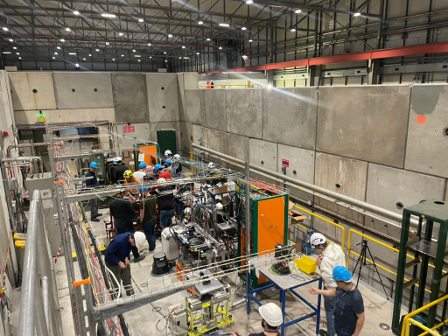
\includegraphics[width=0.75\linewidth]{image.png}
    \caption{Installation of a user experiment in one of the experimental zones on the H8 beamline in the EHN1 building.}
    \label{fig:4.1.1}
\end{figure}

Overall, demand for beam time in our facility is very high and the PS \& SPS Physics Coordinators receive requests from about 100 – 120 different activities for beam time per year from users all over the world. The utilization of the machines is generally above 100\% due to the infrastructure allowing multiple experiments to occur in parallel to each other in several experimental zones (with the new TELMAX beamline not being used to the full capacity yet).

To support the PS \& SPS Physics Coordinators in organizing and handling the requested beam times and manage the user schedule over all beamlines and experimental zones of the facility, a software solution has been developed under the WP 4.4.1 service improvement program. This user schedule management tool was first used for the beam requests in the 2023 beam period and has since then been expanded and integrated into the workflow of user request and change management, reporting of statistics, handling of short-term cancellations and overall communication with the users of the PSSPS facility. Development and maintenance of the tool at least until the end of the beam period in August 2026 has been secured, with additional efforts to investigate opportunities and synergies including a tighter integration and consolidation with other similar management tools at CERN also being investigated and explored. 

Since the start of the project and until the end of reporting period P2, a total of 57 projects applied for funding under the trans-national access (TA) scheme, representing 16004 access units (AU) of delivered beam time in the PSSPS facility and a funding request for a total of 284 users. This represents an increase compared to the numbers for the end of the P1 period (30 projects, 9072 AU, 164 users) of 28 projects, 6932 AU and 120 users. The numbers of P2 also include the first successfully granted application of a user in the new TELMAX beamline. 

Within the objectives and constraints of the WP4 efforts, it was expected that the number of TA applications would decline rather sharply over the runtime of the project. This is due to the high number of activities being associated with the four large LHC experiments, with many of their activities targeting an installation into their respective detectors during the upcoming LS3 shutdown of the CERN accelerator complex. Those activities were expected to mostly transition from R\&D to calibration and quality assurance tasks during reporting periods P2. However, the overall schedule at CERN did change and, with the extension of beam activities until August 2026 and subsequent shift of the LS3, R\&D test beam activities for the LHC experiments targeting installation in LS3 have continued throughout 2024 and, at a significantly decreased rate, are also expected to continue throughout 2025. Additionally, activities targeting subsequent shutdowns (i.e., LS4 or later) and also a number of activities unrelated to the development of LHC detector subsystems continue to perform R\&D tasks. For example, activities under the umbrella of the DRD collaborations are especially worth mentioning here, with first TA applications (3 visits, 936 AU,  13 users) for these groups of users having been filed for the reporting period during 2024. It is therefore expected that the decline in TA applications will be more gradual and less steep than initially anticipated. 

\subparagraph{Sub-task 4.1.2 DESY} \mbox{}

The DESY test beam facility operates at the DESY-II accelerator and is equipped with three test beam lines, providing up to 1,000 particles per cm² with energies from 1 to 6 GeV, an energy spread of ~5\% and a divergence of ~1mrad. Access to these beam lines coupled with extensive technical and administrative user sort is the main objective in the EURO-LABS Transnational Access programme at DESY (WP4.1.2). 

\begin{figure}[!h]
    \centering
    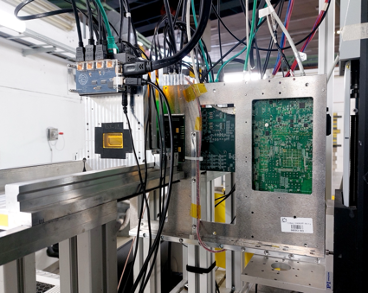
\includegraphics[width=0.75\linewidth]{image2.png}
    \caption{Set-up with RD50-MPW4 D-MAPS CMOS sensor in the DESY II test beam facility. Performance of detectors before and after irradiation was evaluated and compared with results from the previous submission.}
    \label{fig:4.1.2}
\end{figure}

During the second reporting period of the project, 13 user groups with a total of 59 users from 13 different countries have applied for TA. All TA-applications have been approved by the USP. All international teams have been granted in total with 2832 beam-hours of transnational access. 

To ensure the most efficient and transparent support for the user a new automated administrative procedure has been rolled out and is presented in detail on the webpage EURO-LABS at DESY. The processing time for applications and reimbursements has been improved, ensuring timely coverage for all users.

In P1 and P2 of the project, international teams that requested TA support have been granted 4704 beam-hours (AUs) of transnational access in total. 22 projects with a total of 97 users (80 users were funded) from 14 different countries have been granted TA.

\subparagraph{Sub-task 4.1.3 PSI} \mbox{}

The EURO-LABS project in Switzerland could only be started in 2023 as the funds for TA support needed to be confirmed by SERI (State Secretariat for Education, Research and Innovation). The first 4.5 month of the beam period in 2023 were dedicated to a physics experiment, MUSE. Test beams were scheduled for the time after October. Only 2 teams doing test beams applied for TA support: COMET and a group from Mainz and Heidelberg. 

\begin{figure}[!h]
    \centering
    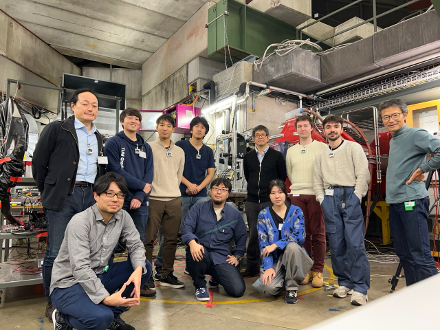
\includegraphics[width=0.75\linewidth]{image3.png}
    \caption{Members of the COMET test beam team at the PiM1 line in PSI, their set-up in the background.  }
    \label{fig:4.1.3}
\end{figure}

The COMET experiment will search for the muon-to-electron conversion process at J-PARC, Japan. This project will primarily involve negative pions, muons, and electrons with a momentum of <200 MeV/c. The primary objective of the test beam was to scrutinise the secondary particles emanating from tungsten blocks, subjected to pions and muons. This analysis was facilitated by a set of plastic scintillating counters. Both tested detectors will contribute to the particle-type identification of these secondary particles. In addition, two COMET detectors, the Range Counter and a prototype of the Cylindrical Trigger Hodoscope were also tested with muon beams in parallel. Those results have also independently contributed to the development of the COMET experiment. 

The group consisted of 12 scientists from Japan, France, and the UK. Five of them - all PhD students - were supported in the framework of the EURO-LABS project.

The second group supported tested a very compact spectrometer consisting of a four-layer pixel detector and a strong permanent neodymium dipole magnet.  This setup serves as a demonstrator for a "photon tracker", where the conversion electron positron pair is tracked in double layers of pixel detectors. The pixel tracker is based on MuPix sensors developed for the Mu3e experiment.

The project was granted two weeks of beam time. Four undergrad-students form the Universities of Heidelberg and Mainz obtained TA support.

In 2024 the schedule was similar to 2023. The PiM1 beam line was dedicated to the MUSE experiment up to mid-August and from the second half of October. Test beams are only scheduled for the time in-between. Several groups have applied for TA funding. Up to end of P2, a total of 11 projects with 32 users were executed, consuming a total of 2808 AUs.

\subparagraph{Sub-task 4.2.1 RBI} \mbox{}

The Tandem Accelerator Facility at the Rudjer Bošković Institute (RBI-AF) is one of the two facilities within the task 4.2 Detector Characterization of WP4. At RBI-AF users can perform:
\begin{itemize}
    \item	in vacuum and in-air IBIC (Ion Beam Induced Charge) imaging of charge collection properties using protons of up to 10 MeV with 1 $\mu$m resolution and heavy ions on demand and/or time resolved IBIC (TRIBIC),
    \item	radiation hardness studies with real-time controlled radiation damage of small detector area using protons or heavier ions, including ion beam analysis.
\end{itemize}
For such studies users can use two ion microprobe end-stations and other end stations, depending on the actual objectives of the proposed work.

In one of the performed TA user projects charge transport response of SiC sensors to harsh environments and to single ion implantation has been studied. The experiment was mostly focused on characterization of world’s first in-line sensor for single ion implantation applications. In the experiment unique capabilities for deterministic heavy ion counting of the novel ultra-thin SiC radiation detectors realized by STLab srl were investigated by users from Switzerland and Italy.

Detailed 3D charge collection efficiency (CCE) characterization of large area single pad SiC detectors dedicated to the use for the particle identification by the MAGNEX focal plane detector within the NUMEN project (double beta-decay study) at LNS Catania were investigated by users from Italy.

CCE characterization of position sensing photodiodes as detectors to determine the impact position of monoenergetic MeV ions was the next subject studied. The spatial resolution and radiation hardness of this position sensitive detector has been characterized by the analysis of experimental data supported by a suitable theoretical model. 

The behaviour and resulting concentration in depth profiles of MeV 7Li ions implanted in novel commercial detector crystalline materials, such as artificial diamond and SiC polytypes was studied. The implantation has been carried out in the axial channeling mode. 

High temperature implantation of Group IV elements into diamond was investigated. Group IV defects in diamond offer a promising platform for applications in quantum technology, quantum sensing and device fabrication, including magnetic field sensors and quantum thermometry. 

\begin{figure} [!h]
    \centering
    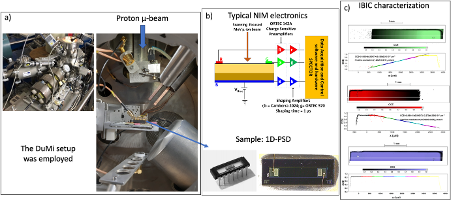
\includegraphics[width=0.75\linewidth]{image4.png}
    \caption{Experiment for the characterization and modification of a 1D-PSD. a) The experiment was carried out at the Dual Microprobe (DuMi) end-station, b) the detectors were read out with NIM-based electronic units, c) IBIC (Ion Beam Induced Charge) microscopy was carried out. After characterization, the detector was modified by means of controlled irradiations aiming to obtain a 2D-PSD response.}
    \label{fig:4.2.1}
\end{figure}

\subparagraph{Sub-task 4.2.2 ITAINNOVA} \mbox{}

During this period, CEA-Saclay requested access to perform a series of tests aimed at characterizing and evaluating the noise susceptibility of the Front-End Electronics (FEE) and DAQ system (ARC) used in the IAXO experiment. ARC currently serves as the reference design for the RadioPure version of the FEE. The IAXO experiment targets the detection of axions in the low-energy range of the spectrum. This requires the MicroMegas detector, the analog signal conditioning stages, and the DAQ system to operate under extremely low electromagnetic noise conditions. Previous issues in IAXO - electronics prototype highlighted the need for this study. Several test campaigns were carried out at EMCLab to support the integration of the improved RadioPure ARC, as shown in Fig. \ref{fig:4.2.2}.

\begin{figure}[!h]
    \centering
    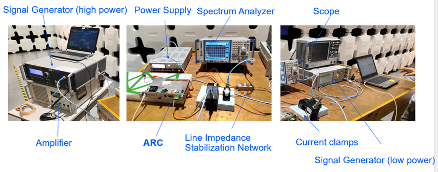
\includegraphics[width=1\linewidth]{image5.png}
    \caption{Detail of the characterization setup of the ARC DAQ in the anechoic chamber.}
    \label{fig:4.2.2}
\end{figure}
The characterizations reported a good immunity of the ARC to conducted noise in the power lines of the electronics. The topological placement of the ASICs in the PCB showed small differences in noise coupling, i.e. noise transfer function (TF) differences between chips. The TF of the input channels has also been studied, enabling the operation of the input stages of the conditioning ASIC in configurations that filter noise for different frequency regions of the input spectrum as it is shown in Fig. \ref{fig:4.2.2a}. The study reports the tunning capabilities of the configuration parameters of the DAQ to cope the noise characteristics at the possible locations where the experiment is studied.

\begin{figure}[!h]
    \centering
    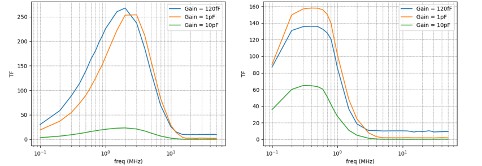
\includegraphics[width=0.75\linewidth]{image6.png}
    \caption{Frequency response of the ARC input for a shaping time of 70 ns (left) and 640ns(right) and different gains on the feedback path.}
    \label{fig:4.2.2a}
\end{figure}
The analogue signal stages prior to the DAQ have been identified as a significant source of noise coupling, with a more pronounced impact than that observed from the DAQ itself. This highlights the need for robust shielding continuity across the entire system, particularly in the Limandes. Several design improvements have already been identified for both the Limandes and the MicroMegas to address this. These findings provide valuable insights for improving the current commissioning of the RadioPure version of the ARC and the detector setup. 

It is important to note that these recent tests have greatly benefited from the latest upgrades. They utilized new tools at the EMCLab, including a Graphical User Interface (GUI) and an automated transfer function (TF) measurement system capable of scanning the setup under various noise and configuration conditions. The tests also confirmed the adaptability and straightforward integration of the GUI and automation with different Front-End Electronics and experimental setups. This is especially relevant as IAXO uses a different hardware system compared to previous experiments tested in the EMCLab, which were primarily focused on CMS-Pixel detectors. 

To date, only three requests for access have been submitted and completed, which represents about 30\% of those initially planned. Although part of the delay is due to the early implementation of technical improvements - planned from the beginning of the project - there has also been a notable slowdown in the submission of new applications. Despite a major promotional effort to highlight the laboratory's capabilities and growing interest in launching new test campaigns, progress has been limited. Two additional applications are currently being prepared, but delays in other projects and the lack of definition of upcoming detector R\&D activities continue to slow down the formalization of new access applications.

\subparagraph{Sub-task 4.3.1 CERN IRRAD} \mbox{}

The proton irradiation facility (IRRAD) at the PS East Area (EA) was built during the Long Shutdown 1 (LS1, 2013-2014) and improved during the LS2 (2019-2021) to cope with the increasing needs for radiation tests of the experimental community working for the HL-LHC upgrade and beyond. The IRRAD facility, operated by EP-DT and exploiting the 24 GeV/c PS proton beam, is part of a more complex infrastructure that includes on the EA-T8 beamline the mixed-field facility CHARM operated by the BE department, the CERN Shielding Benchmark Facility (CSBF test station to benchmark the efficiency of radiation shielding materials), as well as serves as a test bench for developing a high-energy ion beam aiming to provide an optimal tool to reproduce the effects of galactic cosmic rays (within the HEARTS EU-funded project fostered by the CERN-ESA collaboration).

The year 2024 has been the third full year of IRRAD operation after the LS2, 30 user experiments were executed, involving more than 640 samples. About 60\% of the experiments belonged to the CERN LHC Experiments users working to complete the phase II upgrade projects, while the remanet 40\% belonged to CERN equipment groups (ATS), as well as to users from EU/R\&D/external projects. Nine out of the 30 user experiments were performed within the EUROLABS TA framework. Cumulating the EUROLABS TA projects from September 2022 to the end of 2024, a total of 3427 Access Units were provided to 13 selected projects with 32 participating users. With the strong increase of experiments performed in the TA context in 2024, the facility reached already 85\% of the overall pledged EUROLABS Access Units (AUs). The facility is expected to be fully charged in 2025 covering further EUROLABS AUs in parallel to the ongoing radiation hardness and qualification testing for components and detector elements for the HL-LHC various other projects.

\begin{figure}[!h]
    \centering
    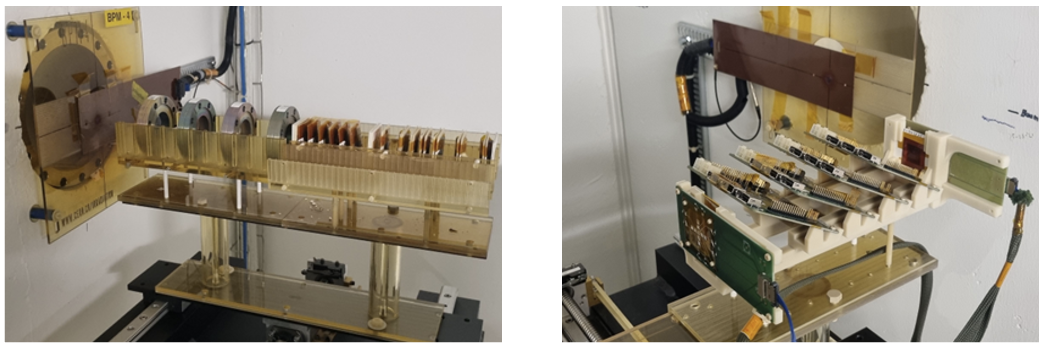
\includegraphics[width=1\linewidth]{image7.png}
    \caption{Examples of experiments performed during the run in 2023 at the IRRAD Facility. Vacuum window samples (left-hand side) and silicon pixel modules (right-hand side).
}
    \label{fig:4.3.1}
\end{figure}

Within the EUROLABS TA framework in P1 and P2 from September 2022 to February 2025 a total of 3247 Access Units were provided to 13 selected projects with 32 participating users. All-in-all, the facility is fully committed in 2025 and 2026 with the EUROLABS TA access. 

\subparagraph{Sub-task 4.3.1 CERN GIF++} \mbox{}
The CERN Gamma Irradiation Facility (GIF++) is a joint BE \& EP Department facility located on the H4 beamline (SPS, Zone PPE-154) in EHN1 hall (North Area, Prevéssin site). It is a unique place for detector R\&D, where a strong $\gamma$-ray source and a muon/pion particle beam 
are simultaneously available. Together with IRRAD in the East Area (Meyrin site), GIF++ delivers essential services to the HEP community, with the focus on validating and optimizing detector technologies, mainly in view of the High-Luminosity upgrade of LHC and accelerator projects beyond.

The irradiator (137Cs, 14 TBq as of 2014) is operated throughout the year, independently of 
the SPS and offers two adjustable gamma irradiation zones, with a total floor space of more than 100 m2 and it is expected to continue, with some limitation, also during the incoming Long Shutdown 3 (LS3). In 2024 the irradiator underwent major corrective/preventive maintenance in order to assure smooth operation over, at least, the next 5 years. A new maintenance contract was also funded and signed. 

\begin{figure}[!h]
    \centering
    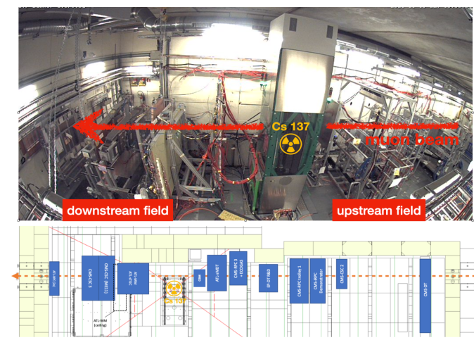
\includegraphics[width=0.75\linewidth]{image8.png}
    \caption{Photograph of the GIF++ irradiation bunker. Up to 11 different setups – often composed of multiple chambers – can be hosted along the muon beam, while several other experiments continue to use the irradiator only. The drawing at the bottom describes the experiments in the experimental area and shows the two opening cones of the gamma irradiator (downstream and upstream fields). }
    \label{fig:4.3.2}
\end{figure}

The two gamma fields (<= 2Gy/h) enable ageing studies and provide radiation background similar to the future working conditions inside the large LHC experiments. The muon (or pion) beam, available during dedicated time slots (typically 3 x 2 weeks/year) is used to investigate and validate the detector performance and behaviour under the expected conditions. During the rest of the year, for about 6 months, the facility is operated using the gamma source alone.

Several groups/set-ups are operated in parallel to optimize/maximize the use of the facility, which is equipped with excellent gas and electronics infrastructures, a unified control/monitoring system, setups for beam and cosmic trigger as well as radiation and environmental conditions monitoring.
The facility is extensively exploited by a large community, mainly composed of users belonging to the CERN LHC experiments. On average, 5 - 6 setups run continuously in parallel during the year, with a peak of 12 setups. In 2024 a campaign to validate the mass production of Resistive Plate Chambers (RPC) for the upgrade of the CMS experiment was started. Discussions are ongoing in order to enlarge the available surface in the bunker.

The extension of the gas area was approved in 2024 and will start in April 2025 to accommodate additional gas systems to cope with the increasing number of user requests. The main detector R\&D programme remains the upcoming upgrade of the LHC experiments in view of the High Luminosity LHC phase (HL-LHC), including long term ageing studies for various gas mixtures, including environmentally friendly ones. 
Over the last years the search for environmentally friendly gas mixtures gained momentum 
and became a driving element of the scientific programme of the facility via the ECOGAS collaboration.

Projects running in the facility require, with a few exceptions, long-term, even years of irradiation and scientists involved spend a large fraction (>50\%) of their working time or are permanently based at CERN.

\subparagraph{Sub-task 4.3.3 JSI} \mbox{}

The reactor facility is used for neutron irradiation to study radiation effects in particle detectors and electronics. The TRIGA reactor provides a unique opportunity for irradiation tests with neutron fluences spanning over many orders of magnitude (Fig. \ref{fig:4.3.3}). For example, electronic circuits containing COTS components were irradiated to 10¹² n/cm², while 3D detector structures were irradiated up to 10$^{18}$ n/cm².

\begin{figure}[!h]
    \centering
    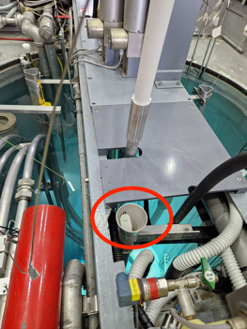
\includegraphics[width=0.6\linewidth]{image9.png}
    \caption{Insertion of samples into the F19 channel (encircled in red) leading to the reactor core faintly visible at the bottom of the water tank. The sample holder can be seen attached to the fishing rope used to lower it for irradiation and then lift it to a shielded position above the core for initial cool-down.}
    \label{fig:4.3.3}
\end{figure}

Since the start of EURO-LABS, 34 projects, totaling 366 Access Units (AU), have been approved by the User Selection Panel. Of these, 31 projects, accounting for 329 AU, were completed by the end of February 2025.

Several projects focused on radiation testing of detectors and electronics for High-Luminosity LHC upgrades. However, the majority were related to the development of charged particle detectors for future applications. These projects included the irradiation of various semiconductor materials such as Si, SiC, GaN, and diamond. Various device types were irradiated – from samples of bulk material (not processed), simple pad diodes to more complicated structures such as 3D detectors, SiPMs, LGADs, AC-LGADs, nLGADs, CMOS DMAPS etc.

A dedicated 120 AU irradiation campaign was organized to expose samples to the extreme fluence of 10$^{18}$ n/cm², to support the development of tracking detectors for future hadron colliders, like FCC-hh. Since irradiation at such high fluences requires significant time and cannot be repeated frequently, a joint irradiation campaign was organized. Samples from twelve institutions were irradiated together over five consecutive days. The high fluences resulted in significant radio-activation, requiring special handling and long cool-down times. Nevertheless, most samples were successfully distributed to test sites, and initial results have already been presented at meetings and conferences. The experience gained in this campaign will be invaluable for the next high-fluence irradiation, which we are planning for this or next year.

\subparagraph{Sub-task 4.3.4 IFJ-PAN} \mbox{}

The AIC-144 cyclotron facility offers 60 MeV proton beams with intensity up to 100 nA in two experimental rooms: a) the former proton therapy eye-treatment room with the setup for precise positioning and clinical-quality irradiation with beam diameters up to 40 mm and b) an experimental hall with an irradiation line equipped with 2D scanner (EURO-LABS service improvement), which allows to expose larger elements with sizes up to 400 mm x 400 mm. It is a user facility, which provides beams for experiments in detector physics, medical physics, cosmic industry and radiobiology. The irradiation stations are equipped with all type of dosimetry tools and are metrologically connected to the Secondary Standard Dosimetry Laboratory in Warsaw.

\begin{figure}[!h]
    \centering
    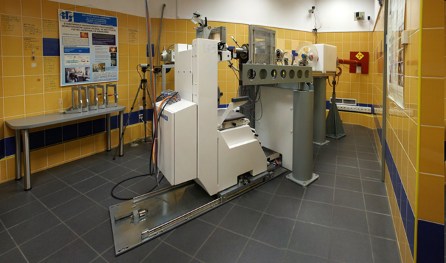
\includegraphics[width=0.75\linewidth]{image10.png}
    \caption{The irradiation room adapted from the proton therapy eye-line installation at IFJ-PAN Krakow. The samples for irradiations are mounted and positioned on the movable treatment chair in front of the beam collimator.}
    \label{fig:4.3.4}
\end{figure}

Within the EURO-LABS project, the facility was mainly used to test detectors intended for use in various experiments in physics and in space. Low gain avalanche detectors (LGAD) were tested for on-line measurements of charged particle flux with high speed and spatial precision. Further projects involved electronic modules of the POLAR-2 Gamma-Ray Burst experiment, Double Sided Silicon Strip Detectors (DS-SSD) for nuclear physics experiments, ion detector systems used for the 10 PW laser-nuclear experiments at ELI-NP and others.  Finally, silicon detectors were irradiated for studies of the defect formation and evolution. These experiments contributed to optimizing silicon detector designs and improving predictions of their behavior for future HEP applications.  Since the start of EURO-LABS 9 projects were supported with 332 access units (cyclotron hours) by EURO-LABS TA.

\subparagraph{Sub-task 4.3.5 UCLouvain} \mbox{}

Cyclotron Research Centre (CRC) is a research unit attached to the Institut de Recherche en Mathematique et Physique (IRMP) at UCLouvain. The facility operates the CYCLONE110 cyclotron, able to accelerate charged ions to kinetic energies up to 110x(Q$^2$/M) MeV. Main activities of the centre are industrial applications (membrane production), and irradiation of electronic components. In total, around 2,500 effective hours of beam are delivered to users during 35 weeks of operation. Around 10\% of access is devoted to scientific applications, mainly nuclear physics experiments, detector irradiations, rad-hard electronic devices and biomedical applications.

\begin{figure}[!h]
    \centering
    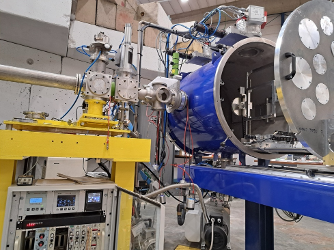
\includegraphics[width=0.75\linewidth]{image11.png}
    \caption{The end of the HIF beam line with the newly installed test chamber }
    \label{fig:4.3.5}
\end{figure}

CRC offers 3 irradiation facilities based on CYCLONE110 operation:
\begin{itemize}
    \item Neutron Irradiation Facility (NIF). Neutrons obtained impinging a 50 MeV deuteron beam on a Be target giving a continuous neutron spectrum up to 50 MeV with a mean energy of 20 MeV. The intensity of the beam can reach a flux of 7.3x10$^{10}$ n s$^{-1}$cm$^{-2}$, providing a beam diameter ~4 cm. Irradiation area can be maintained at constant temperature down to -20$^{\circ}$C during irradiation.
    \item Light Ion Irradiation Facility (LIF). Mono-energetic protons with energies between 20 and 65 MeV. Beam size of ~8 cm diameter and maximum flux of 5x10$^{8}$ p s$^{-1}$cm$^{-2}$.
    \item Heavy Ion Irradiation Facility (HIF). This facility provides a beam of up to 10$^4$ ions s$^{-1}$cm$^{-2}$ monoenergetic heavy ions with well-known range and LET. Irradiation area is ~25 mm diameter with 10\% homogeneity. Various “ion cocktails” can be accelerated allowing an easy and efficient way to change LET. The available cocktails, LET and ranges are described on the facility webpage. This facility is especially devoted to irradiating electronics. DUTs are in vacuum and must not be encapsulated. 
\end{itemize}
All these three facilities are available to EURO-LABS users. So far, for EURO-LABS, we have received just one application, with the irradiation foreseen in spring 2025. 

The installation of the new test chamber for HIF in the scope of the UCLouvain service improvement (Fig. \ref{fig:4.3.5}) has almost been completed. The only piece missing is the installation of a new, scintillator-based detector to cross-check the ion flux measurement. The material has been procured, and it is under test with heavy ions. 

\subparagraph{Sub-task 4.3.6 UoB} \mbox{}

The MC40 cyclotron at the University of Birmingham has been working as a EURO-LABS Transnational Access facility since the beginning of the project. It has delivered irradiations to four projects, and 11 users in total, out of 12 and 36, respectively, requested on the grant. The projects covered the study of radiation damage to depleted Monolithic Active Pixel Sensors, to the I3T80 technology for the development of DC/DC power regulators, to silicon sensors, including novel Low Gain Avalanche Detectors, and the study of effects of annealing on irradiated silicon sensors. 

\begin{figure}[!h]
    \centering
    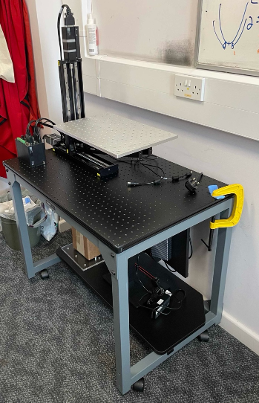
\includegraphics[width=0.5\linewidth]{image12.png}
    \caption{Upgraded sample scanning assembly during the laboratory commissioning phase. }
    \label{fig:4.3.6}
\end{figure}

By the end of the reporting period, about 30 AU were delivered, out of 300 requested on the grant. It must be noted that the MC40 cyclotron has been unavailable for approximately 6 months, between August 2022 and January 2023, due to a fire in one of the magnets that then needed replacement. During these two years, work has been ongoing on system improvements to deliver fluences well above 10$^{16}$ n$_{eq}$/cm$^2$ . The system is in the advanced stages of development (Fig. \ref{fig:4.3.6}) and is approaching a stage where commissioning at the MC40 cyclotron can begin. Full commissioning is planned in May 2025, with routine operations expected to resume in early summer 2025 with a higher fluence capability. This improvement will enable the facility to deliver a higher number of AU to projects and to work towards the delivery of the full AU target (300 AU).

\subparagraph{Task 4.4 Service Improvements} \mbox{}

The Service Improvements (SIs) task WP4.4 comprises ten improvements to facilitate user access at each of the eleven RIs of WP4. Contrary to TA, for SIs EURO-LABS resources were required to be matched by at least the same amount of funding from RIs. Also, the timeline for getting the SIs operational was set at no later than M36 of the project, with a clear preference of getting them on-line sooner to maximize their usage during the project. All but one designs of SIs are documented in their respective milestone reports; the list of SI sub-tasks with their respective target RIs and MS reports follows:
\begin{itemize}
    \item
[4.4.1]	Data base handling of beam time and irradiation requests (4.1.1 CERN TB, 4.3.1 IRRAD \& 4.3.2 GIF++) – MS24
    \item
[4.4.2]	Precision motion stages for large detector setups (4.1.2 DESY test beams) – no MS
    \item
[4.4.3]	Beam monitor (4.1.3 PSI test beams) – MS25
    \item
[4.4.4]	Ion beam focusing lens (4.2.1 RBI-AF) – MS26
    \item
[4.4.5]	Cooling System and Graphical User Interface for EMCI test station (4.2.2 ITAinnova) – MS27
    \item
[4.4.6]	Beam profile monitor (4.3.1 CERN IRRAD) – MS28, MS29
    \item
[4.4.7]	Cadmium shielding in the tangential channel (4.3.3 JSI TRIGA) – MS30
    \item
[4.4.8]	2-D scanning table for irradiation (4.3.4 IFJ-PAN AIC 144) – MS31
    \item
[4.4.9]	Test chamber for the heavy ions irradiation facility (4.3.5 UCL CRC) – MS32
    \item
[4.4.10]	Scanning system upgrade for high fluence delivery (4.3.6 UoB MC40) – MS33
\end{itemize}

\subsubsection*{Main Results and Achievements}
The usage of AUs at the eleven RIs of WP4 during P1 (Sep 22 – Aug 23) and P2 (Sep 23 – Feb 25) is summarized in Table~\ref{tabl:wp4-aunitsp1p2}.

\begin{table}[H]
    \centering
    \caption{Usage of AUs at the WP4 RIs.}
    \label{tabl:wp4-aunitsp1p2}
    \begin{tabular}{|l|*{8}{>{\centering\arraybackslash}p{0.09\textwidth}|}}
        \hline 
        \rowcolor{mycyan} WP4.1 & Name & Pledged & P1	& P2 & P1\&2	& Nominal & P1\&2/ Nominal & P1\&2/ Pledged \\
        \hline
        \rowcolor{white} WP4.1.1	&CERN 	&8736	&9072	&6932	&16004	&5460	&293\%	&183\% \\
        \hline
        \rowcolor{white} WP4.1.2	&DESY	&8640	&1872	&2832	&4704	&5400	&87\%	&54\% \\
        \hline
        \rowcolor{white} WP4.1.3	&PSI	&5376	&0	&2808	&2808	&3360	&84\%	&52\% \\
        \hline
        \rowcolor{mylightergray} Total WP4.1	& &22752	&10944	&12572	&23984	&14220	&165\%	&103\% \\
      
        \hline        
        \rowcolor{mycyan} WP4.2 & Name & Pledged & P1	& P2 & P1\&2	& Nominal & P1\&2/ Nominal & P1\&2/ Pledged \\
        \hline
        \rowcolor{white} WP4.2.1	&RBI	&504	&92	&200	&292	&315	&93\%	&58\% \\
        \hline
        \rowcolor{white} WP4.2.2	&ITAINNOVA	&800	&0	&240	&240	&500	&48\%	&30\% \\
        \hline
        \rowcolor{mylightergray} Total WP4.2	& &1304	&92	&440	&532	&815	&65\%	&41\% \\
      
        \hline   
        \rowcolor{mycyan} WP4.3 & Name & Pledged & P1	& P2 & P1\&2	& Nominal & P1\&2/ Nominal & P1\&2/ Pledged \\
        \hline
        \rowcolor{white} WP4.3.1	&IRRAD 	&4000	&1348	&2079	&3427	&2500	&137\%	&86\% \\
        \hline
        \rowcolor{white} WP4.3.2	&GIF++	&4000	&0	&3744	&3744	&2500	&150\%	&94\% \\
        \hline
        \rowcolor{white} WP4.3.3	&JSI	&700	&78	&245	&323	&437.5	&74\%	&46\% \\
        \hline
        \rowcolor{white} WP4.3.4	&IFJ PAN	&800	&80	&216	&296	&500	&59\%	&37\% \\
        \hline
        \rowcolor{white} WP4.3.5	&UCLouvain	&100	&0	&0	&0	&62.5	&0\%	&0\% \\
        \hline
        \rowcolor{white} WP4.3.6	&UoB &300	&12.5	&25	&37.5	&187.5	&20\%	&13\% \\
        \hline
        \rowcolor{mylightergray} Total WP4.3	& &9900	&1518.5	&6309	&7827.5	&6187.5	&127\%	&79\% \\
        \hline
        \rowcolor{mygray} \textbf{Total WP4	}& &\textbf{33956	}&\textbf{12554.5	}&\textbf{19321	}&\textbf{31875.5	}&\textbf{21222.5	}&\textbf{150\%}	&\textbf{94\%} \\
        \hline
    \end{tabular}
\end{table}

\begin{figure}[!h]
    \centering
    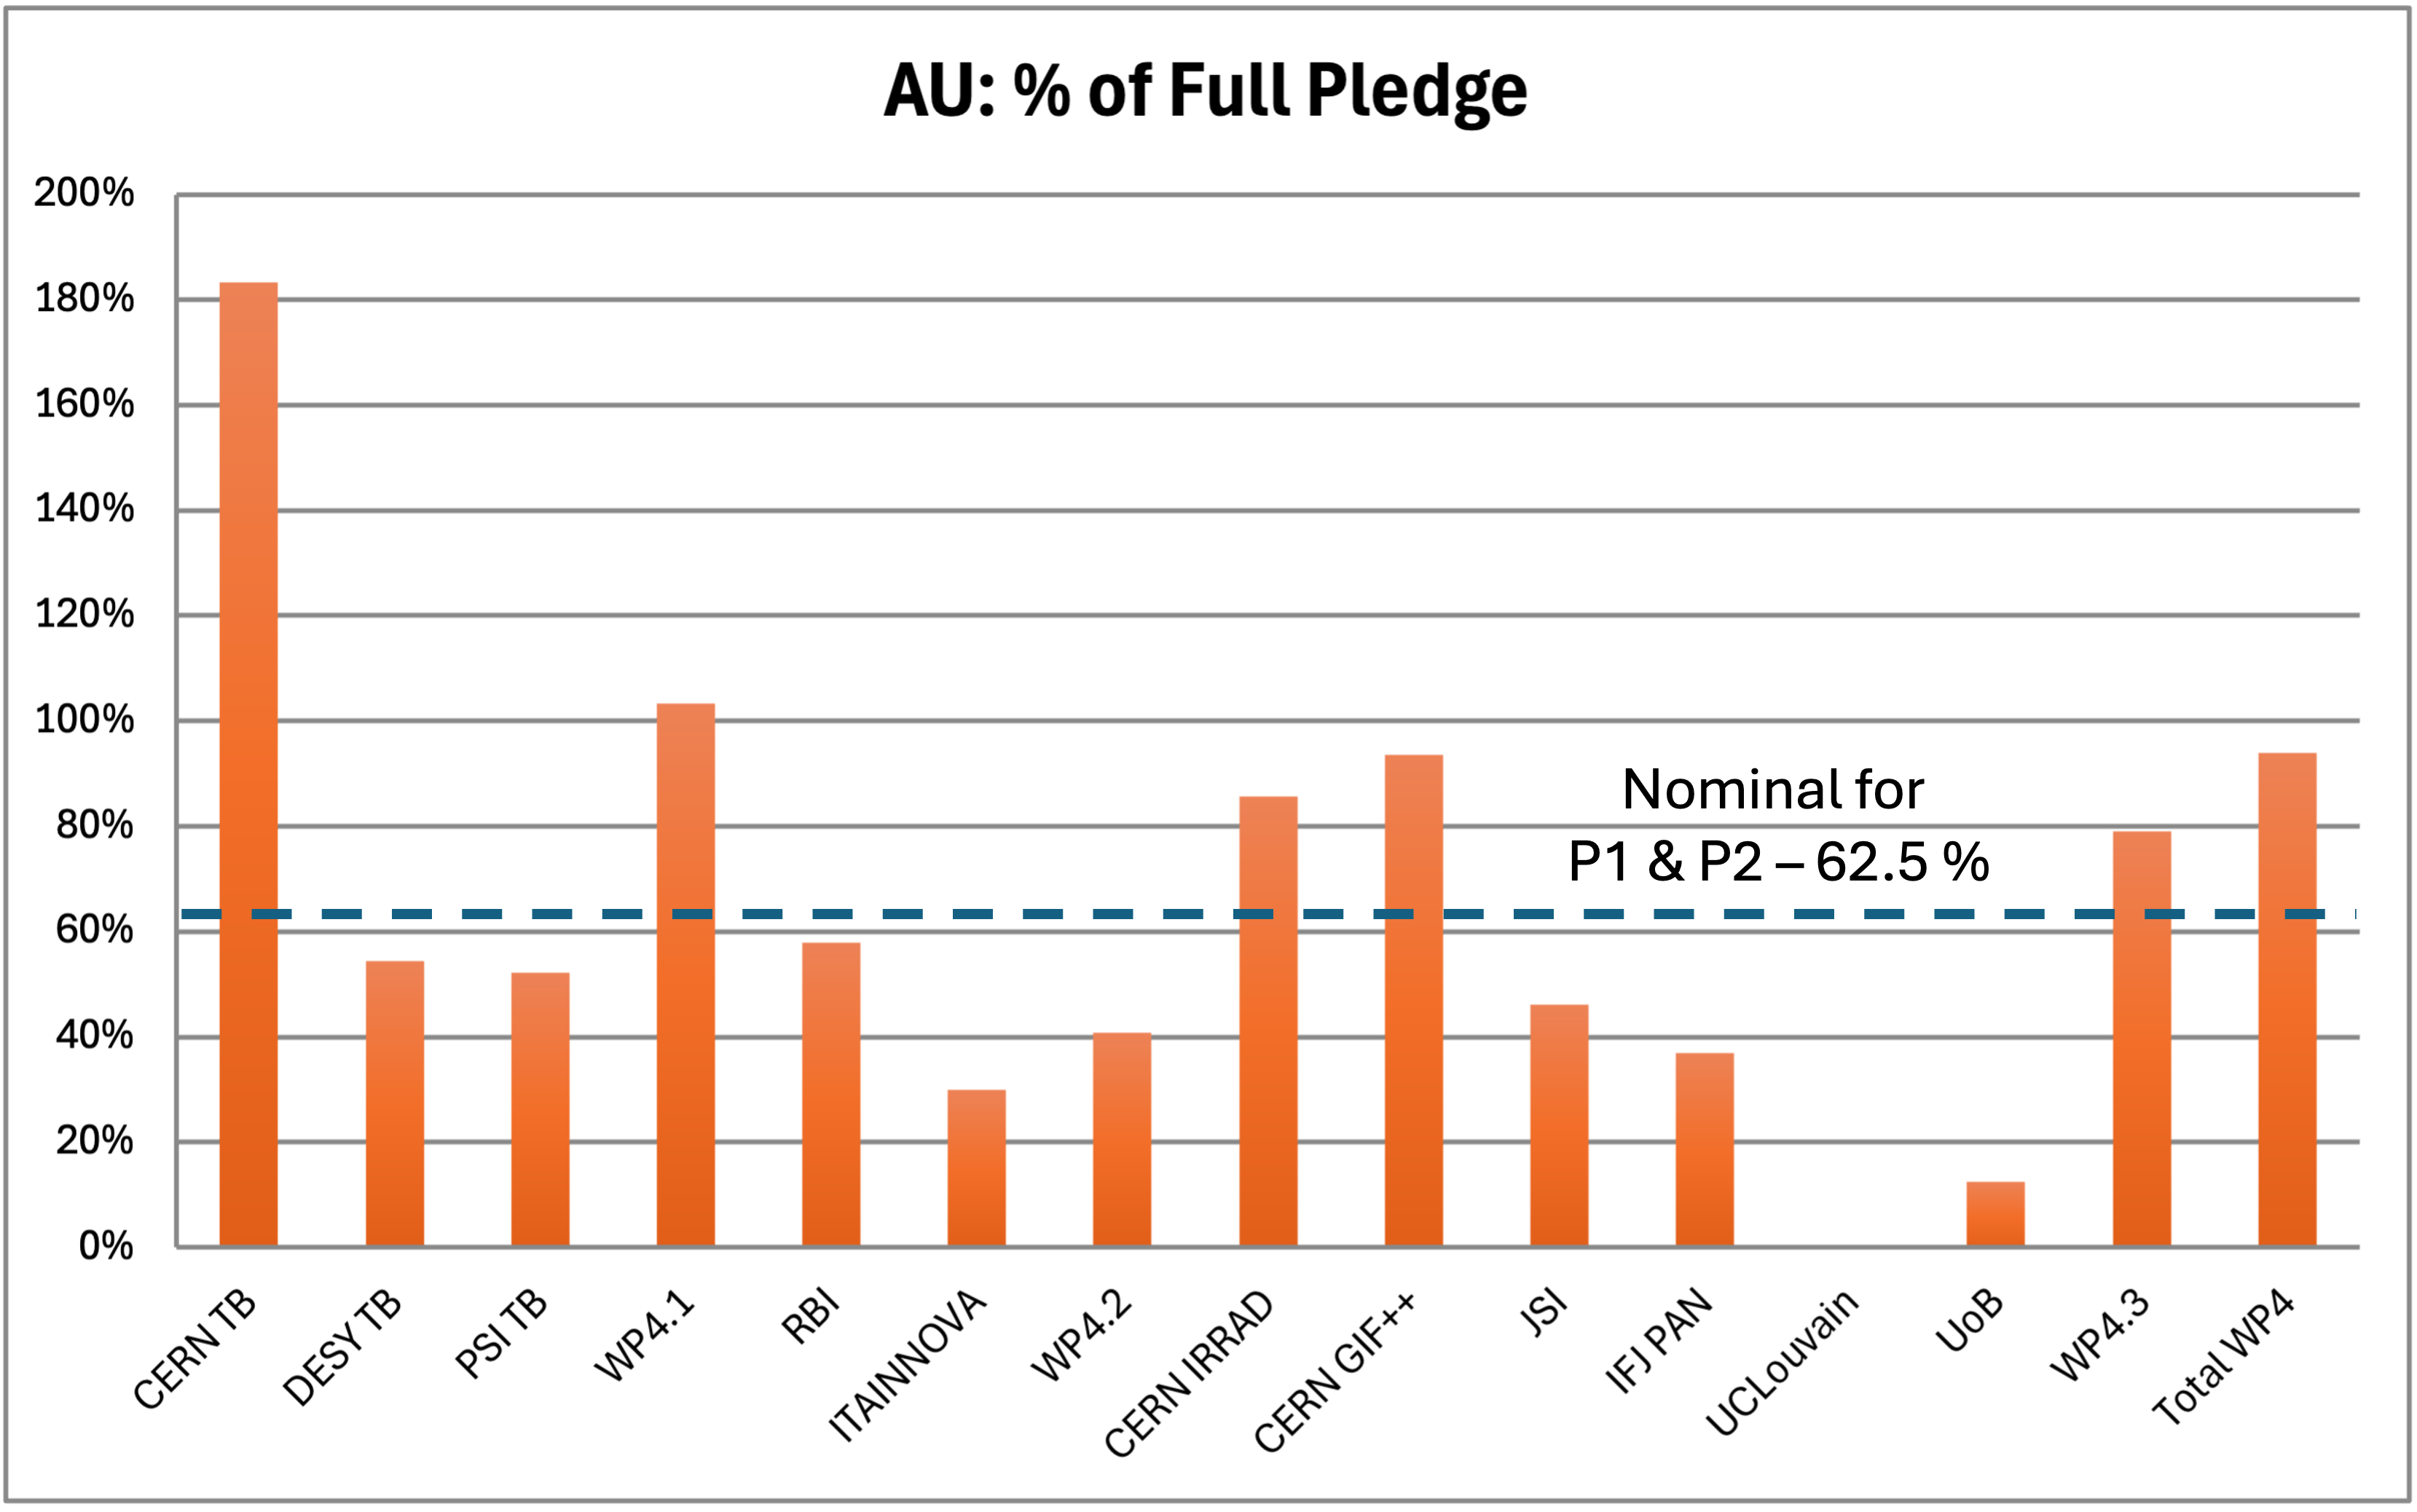
\includegraphics[width=0.75\linewidth]{AU_P12-pledge.png}
    \caption{Delivery of AUs across RIs, tasks and complete WP4. The nominal value for M30 of the project of 62.5\% is ploted as reference.}
    \label{fig:AUs}
\end{figure}

An analysis of more than 100 projects with over 400 users executed during P2 of EURO-LABS in RIs of WP4 reveals a great diversity of the users involved in experiments carried out within the TA framework. Based on the location of their institute  (Fig. \ref{fig:WP4-affiliation}) , the users come from 37 countries on four continents including an almost perfect coverage of EU member states. The distribution of user nationalities  (Fig. \ref{fig:WP4-nationality}) reveals their origin from 43 different countries. The gender balance (Fig. \ref{fig:WP4-gender}) with 21\% of female participation is not ideal, but somewhat typical for the field. The proportion of ECRs (Early Career Researchers), especially for the financially supported users, is very high due to intentional preference of funding students and post-docs.

\begin{figure}[!h]
    \centering
    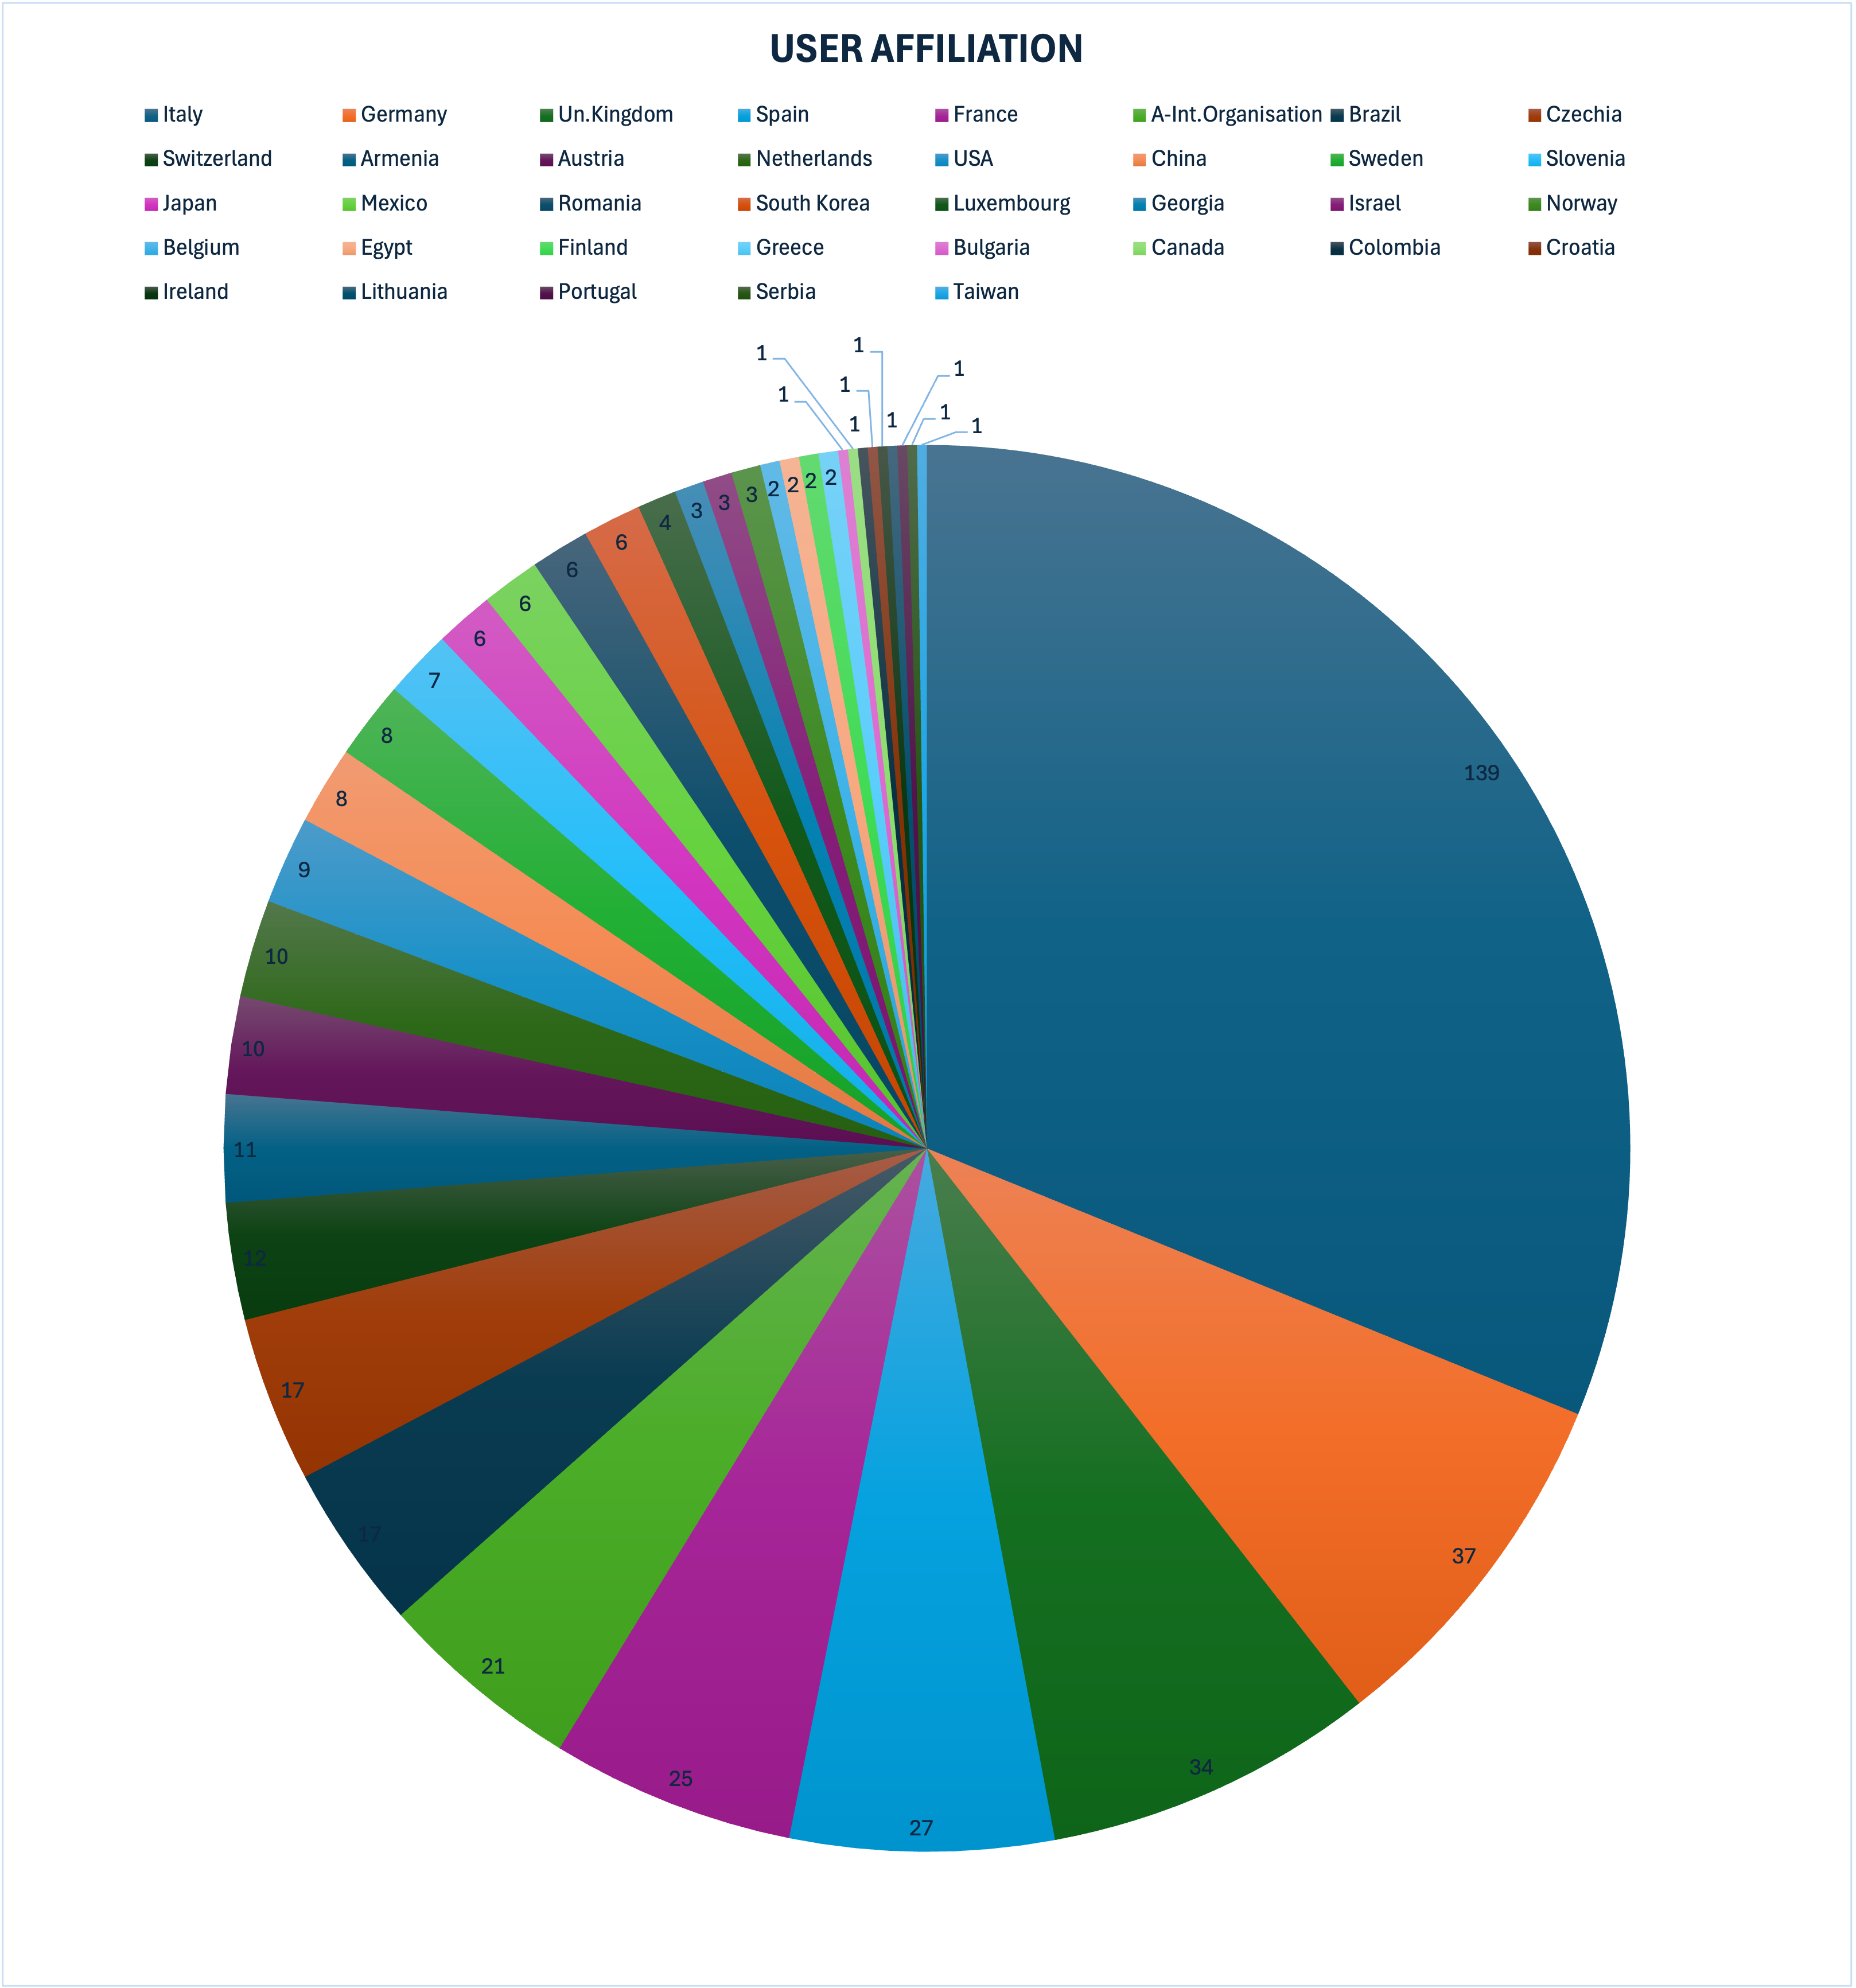
\includegraphics[width=0.75\linewidth]{P2-affiliation.png}
    \caption{Distribution of TA users in WP4 by country of affiliated institute in P2.}
    \label{fig:WP4-affiliation}
\end{figure}

\begin{figure}[!h]
    \centering
    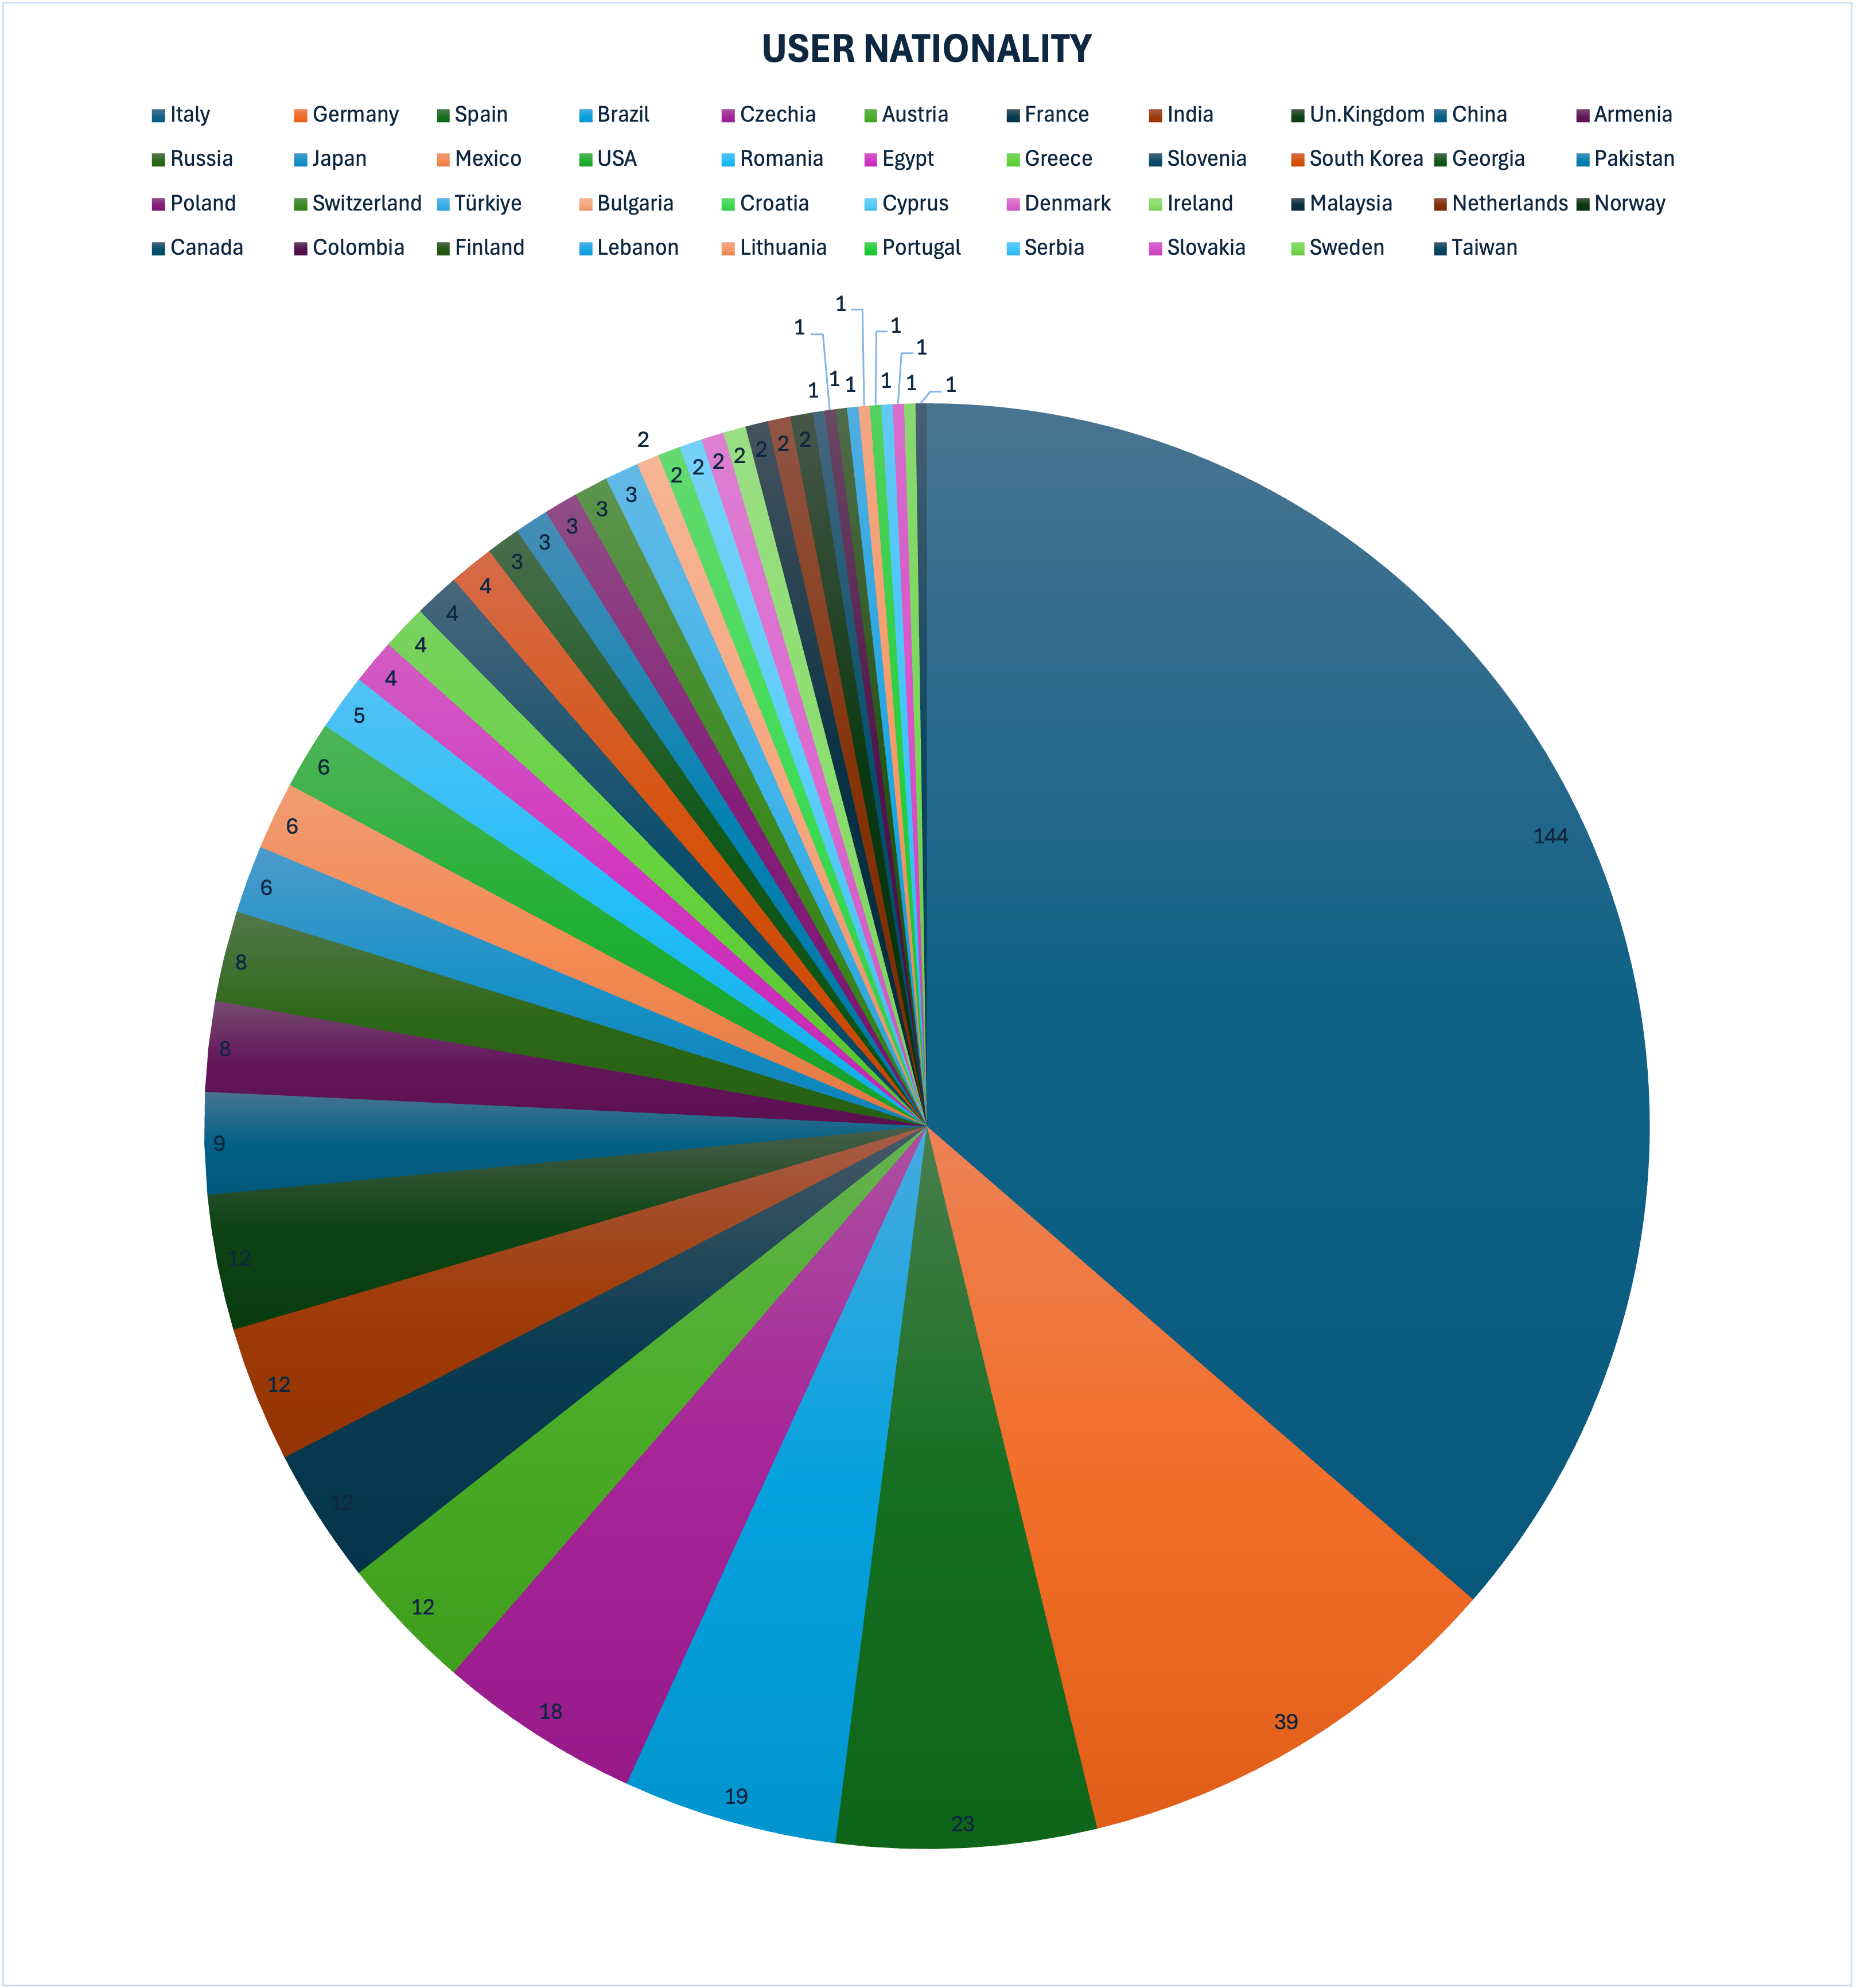
\includegraphics[width=0.75\linewidth]{P2-nationality.png}
    \caption{Distribution of TA users in WP4 by country of origin in P2}
    \label{fig:WP4-nationality}
\end{figure}

\begin{figure}[!h]
    \centering
    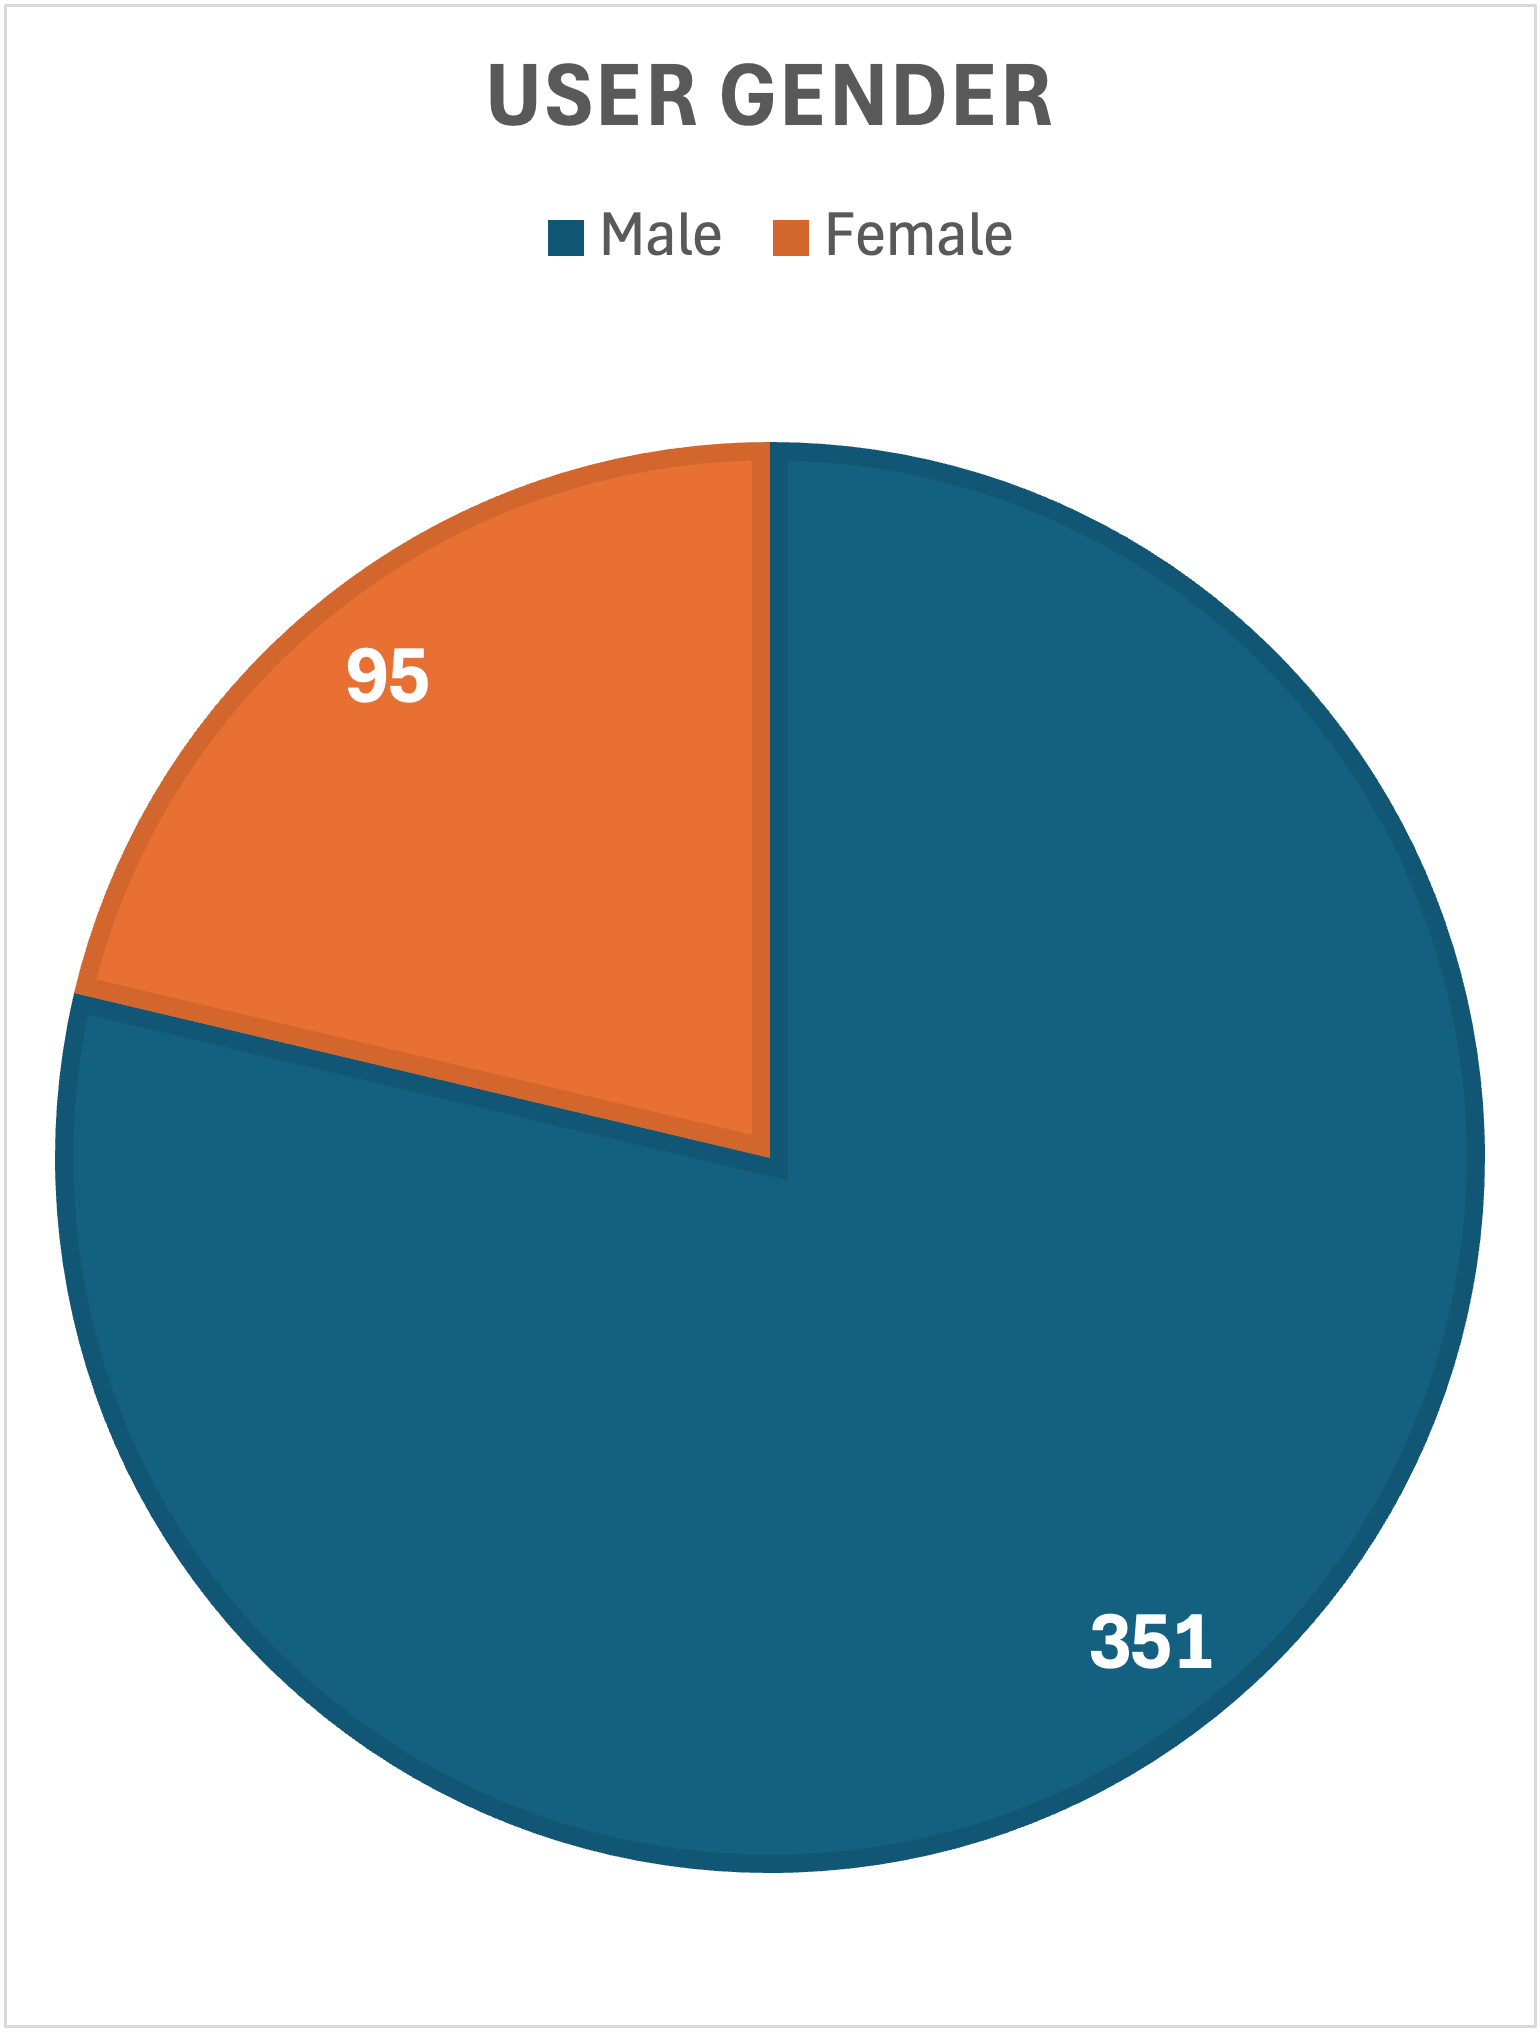
\includegraphics[width=0.5\linewidth]{P2-gender.png}
    \caption{Distribution of 446 WP4 users of TA by gender in P2.}
    \label{fig:WP4-gender}
\end{figure}

\subsubsection*{Deviations and Corrective Actions}
\label{sec:wp4_deviations}

In the remaining 18 months all the three RIs of WP4.1 can be reasonably expected to fulfil their pledge of AU in TA of EURO-LABS. While CERN has already done so, they will continue to deliver AUs to users interested in detector R\&D, as the updated accelerator schedule allows them to continue. DESY is keeping a steady pace towards their target and, barring unforeseen events, can be expected to continue this way. PSI, although experiencing a somewhat slower start, is catching up rapidly and, based on the substantial number of recently submitted applications, is also heading towards timely completion of its contribution.

Up to the end of the project, both RIs of WP4.2 can be expected to fulfil their pledge of AU. For RBI that involves keeping their pace; based on the flow of executed projects their user pool looks relatively stable. At ITTAINNOVA a larger effort is being made to persuade the builders of detector systems to conduct the tests of their detector assemblies at this unique facility. An investment needs to be made to educate the users of the advantages of those tests, best by presenting successful usage cases at internal meetings of the potential user communities.

Even with the overall goal of AU delivery achieved, the relatively meagre performance of some RIs of WP4.3 in delivery of AUs when compared to the nominal, pro-rata expectation calls for consorted action to ensure a successful completion of the project at all RIs. The temporal decline in user interest can be attributed to two facts: 
\begin{itemize}
\item The delays in the detector upgrades for the HL-LHC, which are binding a big pool of potential users to routine QA activities and solving problems that are not in line with genuine detector R\&D.
\item The organization of Detector R\&D (DRD) collaborations as the implementation of the ECFA Detector R\&D Roadmap. That process involved significant effort, effectively reducing the amount of R\&D activity. With all DRDC now in place, we can reasonably expect a boost in their detector R\&D activities. 
\end{itemize}
The construction of the upgrades is bound to last beyond the EURO-LABS project. There are still some modifications that can be regarded as pre-series verification and thus eligible for EURO-LABS support. The major upswing in user demand is though expected to arise from the activity of DRDs. DRD1 (gas detectors) has a large interest in GIF++, DRD3 (solid state) in all RIs (except GIF++) and DRD7 (electronics) in HIF and NIF at UCL (and possibly protons at IFJ-PAN). All the three DRDs were approached, delivering a presentation on EURO-LABS at their respective collaboration workshops. So, it is reasonable to expect an increased user demand for irradiation services, which should allow at task level but also individually at all the six RIs, the pledged amount of AUs to be reached.

\subsubsection*{Milestones and Deliverables}

{\fontsize{9}{11}\selectfont
\begin{center}
  \begin{tabular}[t]{!{\color{mygray}\vrule}p{0.10\linewidth}!
  {\color{mygray}\vrule}p{0.60\linewidth}!
  {\color{mygray}\vrule}p{0.20\linewidth}!{\color{mygray}\vrule} } \hline
    \rowcolor{mycyan} & {\bf Title} & {\bf Status} \\ \hline
    \cellcolor{mycyan}{\bf MS21}: & 4.1 - More than 30\% of AU delivered &  Achieved \\ \hline
    \cellcolor{mycyan}{\bf MS22}: & 4.2 - More than 30\% of AU delivered &  Achieved \\ \hline
    \cellcolor{mycyan}{\bf MS23}: & 4.3 - More than 30\% of AU delivered &  Achieved \\ \hline
    \cellcolor{mycyan}{\bf MS25}: & 4.4.3 	Prototype and software ready for lab tests &  Achieved \\ \hline
    \cellcolor{mycyan}{\bf MS26}: & 4.4.4 	Electrostatic Microprobe Quadrupole Quadruplet Lens Assembly installed and tested &  Achieved \\ \hline
    \cellcolor{mycyan}{\bf MS27}: & 4.4.5 	Cooling system developed &  Achieved \\ \hline
    \cellcolor{mycyan}{\bf MS29}: & 4.4.6 ML-based classification and evaluation of the beam profile patterns &  Achieved \\ \hline
    \cellcolor{mycyan}{\bf MS30}: & 4.4.7 	Design of the shielding system including safety related aspects &  Achieved \\ \hline
    \cellcolor{mycyan}{\bf MS31}: & 4.4.8 	Design of the XY table and purchase of materials and equipment for the device &  Achieved \\ \hline
    \cellcolor{mycyan}{\bf MS32}: & 4.4.10 Mechanics of the setup adapted to fit into the experimental area &  Achieved \\ \hline

  \end{tabular}
\end{center}
}

\subsubsection*{Project Meetings}
\begin{table}[H]
    \centering
    \caption{Summary of WP4-specific meetings in P2.}
    \begin{tabularx}{\textwidth}{|c|c|c|X|} \hline
        \rowcolor{mycyan}
        \textbf{Date} & \textbf{Meeting} & \textbf{Place} & \textbf{URL} \\ \hline
        18/9/2023 & WP4 quarterly meeting & Zoom & https://agenda.infn.it/category/1607/ \\ \hline         10/10/2023 & WP4 meeting during SAM & Krakow & https://agenda.infn.it/event/34651/ \\ \hline 
        25/3/2024 & WP4 quarterly meeting & Zoom & https://agenda.infn.it/category/1607/  \\ \hline        15/7/2024 & WP4 quarterly meeting & Zoom & https://agenda.infn.it/category/1607/ \\ \hline 
        29/10/2024 & WP4 meeting during TAM & CERN & https://indico.cern.ch/event/1370378/ \\ \hline 
        20/1/2025 & WP4 quarterly meeting & Zoom & https://agenda.infn.it/category/1607/ \\ \hline
     \end{tabularx}
    \label{tab:meetings}
\end{table}
%  {\color{mygray}\vrule}p{0.40\linewidth}!

%%%%%%%%%%%%%%%%%%%%%%%%%%%%%%%%%%%%%%%%%
%%%%%%%%%%%%%%%%%%%%%%%%%%%%%%%%%%%%%%%%%
%%% WP01
%%%%%%%%%%%%%%%%%%%%%%%%%%%%%%%%%%%%%%%%%

\tsubsubsection{WP05 - Open Diverse and Inclusive Science}

%%%%%%%%%%%%%%%%%%%%%%%%%%%%%%%%%%%%%%%%%
%%% Section content, please change!
%%%%%%%%%%%%%%%%%%%%%%%%%%%%%%%%%%%%%%%%%

\subsubsection*{Overview and Goals}

\begin{table}[H]
    \renewcommand{\arraystretch}{1.50}		
    \footnotesize   
    \begin{tabular}{*{3}{|p{0.10\textwidth}}|l|}
        \hline
        \rowcolor{mygray} \multicolumn{4}{|c|}{\textit{\color{white}Work Package Summary}} \\
        \hline
        \rowcolor{mylightergray} \textit{WP 5} & \cellcolor{white} 01 & \textit{Title of WP} & \cellcolor{white} Open Diverse and Inclusive Science \\
        \hline
        \rowcolor{mylightergray} \textit{Start} & \cellcolor{white} Mxx & \textit{End} & \cellcolor{white} Myy \\
        \hline
        \rowcolor{mylightergray} \multicolumn{4}{|p{0.978\textwidth}|}{\textit{Participating Organisations}} \\
        \hline
        \multicolumn{4}{|p{0.978\textwidth}|}{
            \hspace*{-0.75cm} 
            \begin{minipage}[t]{\textwidth}
    			\begin{itemize}
    			    \item WP Leader: Partner 1
    				\item Participants: Partner 2, Partner 3, Partner 4, Partner 5, Partner 6, Partner 7
    			\end{itemize} 
    			\vspace*{0.10em}
			\end{minipage}
        } \\
        \hline
    \end{tabular}
    \vspace{0.5em}\vfill
    \begin{tabular}{|p{0.978\textwidth}|}
        \hline
        \rowcolor{mylightergray} \textit{Goals} \\
        \hline
        \rowcolor{white} 
        \hspace*{-0.75cm} 
        \begin{minipage}[t]{\textwidth}
    		\begin{itemize}
    		    \item Goal 1
    			\item Goal 2
			    \item Goal 3
    		\end{itemize} 
    		\vspace*{0.10em}
		\end{minipage}        
        \\
        \hline
    \end{tabular}
    \vspace{0.5em}\vfill
    \begin{tabular}{|l|*{7}{>{\centering\arraybackslash}p{0.084\textwidth}|}}
        \hline    
        \rowcolor{mylightergray} \textit{Participant number} & \textit{1} & \textit{2} & \textit{3} & \textit{4} & \textit{5} & \textit{6} & \textit{7} \\
        \hline
        \rowcolor{white} \cellcolor{mylightergray}\textit{Participant short name} & Partner 1 & Partner 2 & Partner 3 & Partner 4 & Partner 5 & Partner 6 & Partner 7 \\
        \hline
        \rowcolor{white} \cellcolor{mylightergray}\textit{PM per participant} & xx & xx & xx & xx & xx & xx & xx \\
        \hline        
    \end{tabular}    
\end{table}

\subsubsection*{Status}

\todo{Briefly explain the status of the WP.}

\subsubsection*{Progress per Task}

\subparagraph{Task 5.2: Open Science } \mbox{}
\todo{Work In Progress}

Within WP5, the goal of the Task 5.2 is to provide new services to the users in order to achieve an improved and facilitated access to experimental dataset produced in Research Infrastructures. The services aims at improved FAIR data practices. This includes (1) a new data catalog (openNP), (2) an authentification and authorization (AAI) service and (3) a prototype of plateform for data access.

During the reporting period for the sub tasks, the main results are :
\begin{itemize}
    \item  release of the specification document of the openNP catalog under MS35.
    \item the AAI service based on INDIGO-IAM was published online (https://iam-eurolabs.ijclab.in2p3.fr/) and is now being used by the Virtual Access platform Theo4Exp of the EURO-LABS Project (Task 2.4) to authentify their users. To date, more than 250 users are registered and the services is used for the authentication various services (Theo4NP (Task of EURO-LABS), grafana monoriting services at GSI and GANIL) Promotion of the service to future user was achieved.
    \item Different data lake prototypes are being developed/tested based also in coordination with the ESCAPE Project and the PUNCH4NFDI project. The results from these prototypes combined with the other related activities like AAI, will lead to a federated infrastructure concept that will be implemented in FAIR and other infrastructures.
    \item An advanced training school on data management was organized under EURO-LABS WP5.4 and the HGS-HIRe doctoral school in Nov 2024. Lectures and Hands on material can be found in  : \url{https://indico.gsi.de/event/19808/}. The material produced by the school attendees was also published on the zenodo repository of the project. 
\end{itemize}

In addition, under Task 5.2, the Data Management Plan of the EURO-LABS project was reviewed and updated (D5.8).

Digital objects (reports, deliverables, communications, ...) produced by the project can be found on the zenodo repository of the project (\url{https://zenodo.org/communities/euro-labs}). 

\subparagraph{Task 5.3: Machine Learning (Month xx-yy)} \mbox{}


\todo{Work in Progress}

Within WP5, the Task 5.3 aims to use Machine Learning (ML) methods to improve beam characteristics, transport efficiency, and reproducibility of accelerator tuning, which will reduce the beam preparation time and thus the available time for the experiments. Accelerator laboratories worldwide are exploring a large variety of techniques to achieve this aim, from classical optimization and Bayesian optimization (BO) to reinforcement learning. One part of this automation effort is to provide a framework that allows machine experts, operators, and users to solve certain, focused optimization problems and to make these solutions reusable in an operational context. We call this project the “Generic Optimization Framework and Frontend”, or Geoff for short.  EURO-LABS finances one scientific staff
member at GSI for three years for deployment and implication of Geoff for improved beam delivery at EURO-LABS facilities.

The main result of Task 5.3 is the regular use of Geoff at two facilities, CERN (Switzerland) and GSI (Germany). Its successful application to improve accelerator tuning at GSI has been demonstrated in several dedicated beam experiments. The beam loss of the injection into the SIS18 synchrotron has been reduced from 40$\%$ to 15$\%$ in about 15 minutes, where manual tuning can take up to 2 hours. Geoff has also been successfully applied to the GSI Fragment Separator (FRS) for beam steering and focusing, see Figure~\ref{fig:wp5_frs}. In particular, the great flexibility of Geoff, allowing the integration of new and legacy control systems, has significantly facilitated and accelerated the application of ML methods at GSI. 

\begin{figure}
    \centering
        \begin{tikzpicture}
        \node[above] (vis) at (0.0, 0.0) {%
            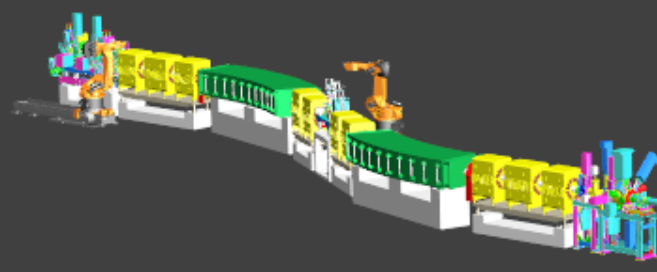
\includegraphics[width=0.45\textwidth]{graphics/wp5_gsi_frs_vis-3d.png}%
        };
        \node[below right] (obs) at (1.0, -1.0) {%
            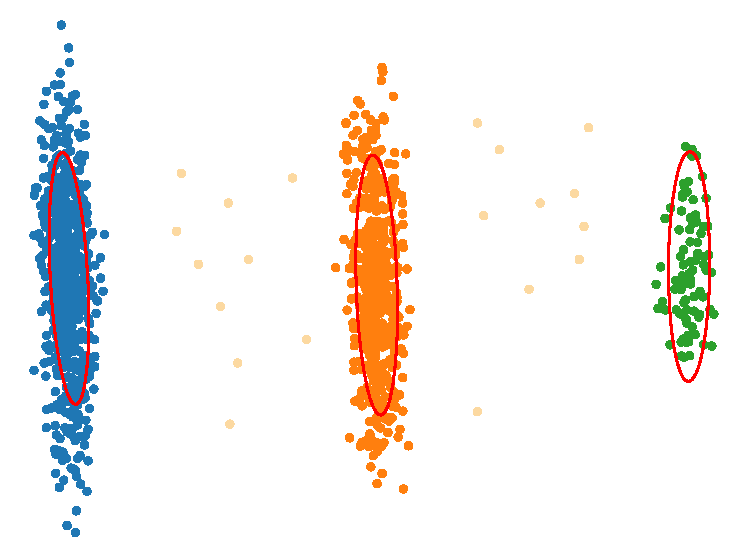
\includegraphics[width=0.20\textwidth]{graphics/wp5_gsi_clusters-speckled.pdf}%
        };
        \node[below left] (res) at (0.0, -0.7) {%
            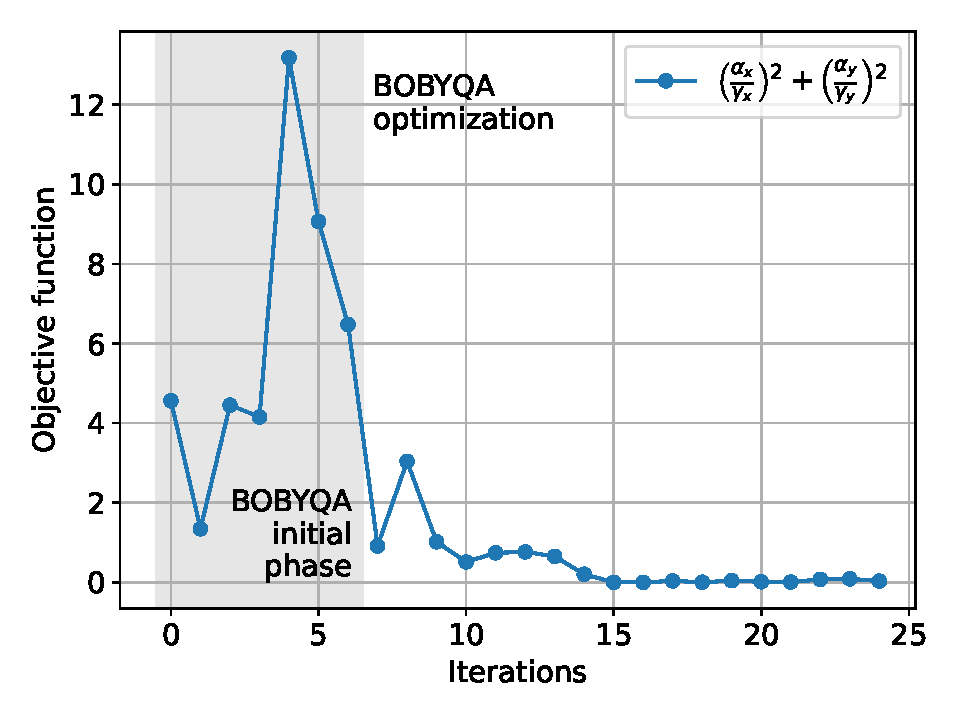
\includegraphics[width=0.31\textwidth]{graphics/wp5_gsi_bobyqa.pdf}%
        };
        \path[use as bounding box] (res.south west) (vis.north) (obs.south east);
        \begin{scope}[node font=\scriptsize\bfseries, above, inner sep=0]
            \node (vis title) at (vis.north) {Illustration of FRS Dispersive Area};
            \node (obs title) at (obs.north) {TPC Data Dnalysis};
        \end{scope}
        \node[
        draw=orange,
        ultra thick,
        circle,
        minimum width=1.2cm,
        minimum height=1.4cm,
        ] (quads) at (1.9, 0.9) {};
        \begin{scope}[->, >=Triangle, draw=blue, ultra thick, node font=\tiny]
            \draw (obs) -- (obs -| res.east)
            node[midway, above, align=center, text width=1.5cm, outer sep=3pt] {%
                evaluation of beam spot slope%
            };
            \draw (res.60) -- (quads)
            node[pos=0.6, text=white, above left, align=center, outer sep=auto] {%
                change\\quadrupole\\strengths%
            };
            \draw (quads) -- (obs title);
        \end{scope}
    \end{tikzpicture}
    \caption{Automatic online focusing for the GSI Fragment Separator (FRS) that uses the BOBYQA algorithm. The gray area in the left figure marks the initialization phase of the algorithm. Convergences has been reached after about 15 iterations. The objective function (left figure, legend) is a scalar measure of how vertical the U91+ beam spot is oriented (right figure). The BOBYQA algorithm optimizes the strength of the quadrupole magnets (top figure).}
    \label{fig:wp5_frs}
\end{figure}

The adaptation of Geoff to a laser-driven particle accelerator
at CEA (France) has started in  November 2024. A majority of the work will be carried out by the post-doctoral researcher financed by Euro-Labs in collaboration with GSI and CERN. The firts tests on the LPA-UHI100 facility ( part of the facilities offering beamtime through WP3) will start as soon as the final authorization to shoot full energy on target will be given by ASN (Nuclear Safety Authority)/CEA. 

\subparagraph{Task 5.4: Training (Month xx-yy)} \mbox{}

\todo{Briefly explain the progress of the task in context to the DoA.}
Within WP5, Task 5.4 aims to assure and improve the participation of new generations of scientists by the yearly organization of basic and advanced training schools, hosted by different beneficiary institutions of EURO-LABS, as well as the identification and partial support of other training events that are organized in Europe in order not to duplicate efforts. We have proposed to have four Basic Training School (BTS) and four Advanced Training School (ATS), and in addition to support events organized by Beneficiaries of EURO-LABS that fit the scope of our training Task 5.4.
So far we have organised two basic schools: BTS23 in September 13$^{th}$–23$^{rd}$, 2023, at IFIN-HH, Bucharest-Magurele, Romania ((https://indico.nipne.ro/event/246/) and BTS24 in June 18$^{th}$-27$^{th}$ 2024, in Warsaw, Poland(https://www.slcj.uw.edu.pl/en/bts24/), hosted by HIL and ICST, Warsaw and two advanced schools: ATSOA (Advanced training School on Operation of Accelerators in June 3$^{rd}$ -7$^{th}$, 2024, at CERN (https://indico.cern.ch/event/1357293/) and Advanced School on Open Science and Data Management in Nov. 24$^{th}$-27$^{th}$, at GSI/FAIR, Darmstadt, Germany (https://indico.gsi.de/event/19808/). All information about the school can be reached from the EURO-LABS web site. The details are also included in the deliverable D5.5 "Report on activities after 2 years, including follow-up from participants" (August 31, 2024). All of these schools were well attended by students and young researchers from Europe and other continents and were very much appreciated. The hosts asked the participants to answer questions that were later used to better organize the next events. 

Additionally, EURO-LABS has supported (co-sponsored) the “R-matrix school” in Edinburgh and the Nuclear Physics for Astrophysics NPA XI school in Dresden, Sep. 9-15, 2024. In its latest meeting TSB has approved tho organization of the remainder two BTS schools at CNA Seville in June 2025 and IFIN-HH in May 2026. TSB reviewed further requests for support (co-sponsorship) from The NIC XVIII school, Barcelona, June 2025, and the Carpathian Summer School of Physics, Sinaia, June 2025. Both requests were accepted and the events are being organized right now.


Currently we are working on the new edition of the advance school in accelerators, ATSOA25 that will take place in May 12$^{th}$-16$^{th}$ at CERN. We had 32 application and 20 trainees were selected. The basic School on Accelerator Applications, BTS25, will take place in Seville from 3rd to 9th of June[https://indico.cern.ch/event/1482911/]. The period for application close March 3rd.

All events organized or supported so far were very successful, based on the number of participants, and their positive feedback. The organizers and trainers, have seen how such events can be even better organized and planned to further increase the impact for the youngsters.
Below are some of the major feedback that was received:
- Hands-on events are most appreciated by trainees
- Diversity of equipment and installations used was well appreciated by those who are at the point     of choosing a career path for their upcoming careers.
- Basic Schools of 10-12 days long allow the trainees to work directly and to know each-other, 
We noticed that Younger scientists are the most appreciated trainers

\subsubsection*{Main Results and Achievements}

\todo{Briefly summarise the main results and achievements of the WP in context of the DoA.}
Activities under Task 5.4 started with the selection of a Training Scientific Board (TSB), completed by Feb. 2023. The activities that followed were in agreement with the initial proposal and overseen by TSB. Basic Training Schools (BTS) and Advanced Training Schools on Operation of Accelerators (ATSOA) were organized:

BTS23 at IFIN-HH, Bucharest-Magurele, Romania

BTS24, at HIL and INC, Warsaw, Poland

ATSOA24 at CERN, Geneve, Switzerland / France

ATSOSDM24 by GSI/FAIR, Darmstadt, Germany

ATSOA25, at CERN - organization in progress

BTS25 in Seville, Spain - organization in progress.

Two schools were co-sponsored in 2024 and two more were approved for sponsorship in 2025.
\subsubsection*{Deviations and Corrective Actions}

\todo{Briefly summarize any deviations and performed corrective actions of the WP in context of the DoA.}
Organizers asked the young participants to judge the events and activities they attended. They appreciated most the hands-on activities and that was strengthened. When confronted with applications from students from other continents (America, Africa) for which we feared we will not have sufficient funds, we have learned that the applicants could come with travel support from their home institutions. That enlarged the reach of the events and of EURO-LABS to the international communities. We have also learned that common extra-curricula activities bind very much the young participants and their hosts.
\subsubsection*{Milestones and Deliverables}

{\fontsize{9}{11}\selectfont
\begin{center}
  \begin{tabular}[t]{!{\color{mygray}\vrule}p{0.10\linewidth}!
  {\color{mygray}\vrule}p{0.60\linewidth}!
  {\color{mygray}\vrule}p{0.20\linewidth}!{\color{mygray}\vrule} } \hline
    \rowcolor{mycyan} & {\bf Title} & {\bf Status} \\ 

    \hline
    \cellcolor{mycyan}{\bf D5.1}: & All research  infrastructures videos completed & Achieved \\
    \hline
    \cellcolor{mycyan}{\bf D5.4}: & The new toolkit deployed at least two facilities and been used optimization  & Achieved \\
    \hline
    \cellcolor{mycyan}{\bf D5.5}: & Report on Training Activities after 2 years including followup from participants & Achieved \\ 
    \hline
    \cellcolor{mycyan}{\bf D5.8}: & Data Management Plan – Interim release  & Achieved \\ 
    \hline
  \end{tabular}
\end{center}
}

\subsubsection*{Project Meetings}

%  {\color{mygray}\vrule}p{0.40\linewidth}!

%%%%%%%%%%%%%%%%%%%%%%%%%%%%%%%%%%%%%%%%%
%%%%%%%%%%%%%%%%%%%%%%%%%%%%%%%%%%%%%%%%%
%%% WP01
%%%%%%%%%%%%%%%%%%%%%%%%%%%%%%%%%%%%%%%%%

\tsubsubsection{WP06 - Ethic Requirements}

%%%%%%%%%%%%%%%%%%%%%%%%%%%%%%%%%%%%%%%%%
%%% Section content, please change!
%%%%%%%%%%%%%%%%%%%%%%%%%%%%%%%%%%%%%%%%%

\subsubsection*{Overview and Goals}

\begin{table}[H]
    \renewcommand{\arraystretch}{1.50}		
    \footnotesize   
    \begin{tabular}{*{3}{|p{0.10\textwidth}}|l|}
        \hline
        \rowcolor{mygray} \multicolumn{4}{|c|}{\textit{\color{white}Work Package Summary}} \\
        \hline
        \rowcolor{mylightergray} \textit{WP No.} & \cellcolor{white} 01 & \textit{Title of WP} & \cellcolor{white} WP Title \\
        \hline
        \rowcolor{mylightergray} \textit{Start} & \cellcolor{white} Mxx & \textit{End} & \cellcolor{white} Myy \\
        \hline
        \rowcolor{mylightergray} \multicolumn{4}{|p{0.978\textwidth}|}{\textit{Participating Organisations}} \\
        \hline
        \multicolumn{4}{|p{0.978\textwidth}|}{
            \hspace*{-0.75cm} 
            \begin{minipage}[t]{\textwidth}
    			\begin{itemize}
    			    \item WP Leader: Partner 1
    				\item Participants: Partner 2, Partner 3, Partner 4, Partner 5, Partner 6, Partner 7
    			\end{itemize} 
    			\vspace*{0.10em}
			\end{minipage}
        } \\
        \hline
    \end{tabular}
    \vspace{0.5em}\vfill
    \begin{tabular}{|p{0.978\textwidth}|}
        \hline
        \rowcolor{mylightergray} \textit{Goals} \\
        \hline
        \rowcolor{white} 
        \hspace*{-0.75cm} 
        \begin{minipage}[t]{\textwidth}
    		\begin{itemize}
    		    \item Goal 1
    			\item Goal 2
			    \item Goal 3
    		\end{itemize} 
    		\vspace*{0.10em}
		\end{minipage}        
        \\
        \hline
    \end{tabular}
    \vspace{0.5em}\vfill
    \begin{tabular}{|l|*{7}{>{\centering\arraybackslash}p{0.084\textwidth}|}}
        \hline    
        \rowcolor{mylightergray} \textit{Participant number} & \textit{1} & \textit{2} & \textit{3} & \textit{4} & \textit{5} & \textit{6} & \textit{7} \\
        \hline
        \rowcolor{white} \cellcolor{mylightergray}\textit{Participant short name} & Partner 1 & Partner 2 & Partner 3 & Partner 4 & Partner 5 & Partner 6 & Partner 7 \\
        \hline
        \rowcolor{white} \cellcolor{mylightergray}\textit{PM per participant} & xx & xx & xx & xx & xx & xx & xx \\
        \hline        
    \end{tabular}    
\end{table}

\subsubsection*{Status}

\todo{Briefly explain the status of the WP.}

\subsubsection*{Progress per Task}

\subparagraph{Task no: title (Month xx-yy)} \mbox{}

\todo{Briefly explain the progress of the task in context to the DoA.}

\subparagraph{Task no: title (Month xx-yy)} \mbox{}

\todo{Briefly explain the progress of the task in context to the DoA.}

\subsubsection*{Main Results and Achievements}

\todo{Briefly summarise the main results and achievements of the WP in context of the DoA.}

\subsubsection*{Deviations and Corrective Actions}

\todo{Briefly summarise any deviations and performed corrective actions of the WP in context of the DoA.}

\subsubsection*{Milestones and Deliverables}

{\fontsize{9}{11}\selectfont
\begin{center}
  \begin{tabular}[t]{!{\color{mygray}\vrule}p{0.10\linewidth}!
  {\color{mygray}\vrule}p{0.60\linewidth}!
  {\color{mygray}\vrule}p{0.20\linewidth}!{\color{mygray}\vrule} } \hline
    \rowcolor{mycyan} & {\bf Title} & {\bf Status} \\ \hline
    \cellcolor{mycyan}{\bf D1.x}: &  &  \\ \hline
  \end{tabular}
\end{center}
}

\subsubsection*{Project Meetings}

%  {\color{mygray}\vrule}p{0.40\linewidth}!

%%%%%%%%%%%%%%%%%%%%%%%%%%%%%%%%%%%%%%%%%
% \input{sections/WPxy}

%%%%%%%%%%%%%%%%%%%%%%%%%%%%%%%%%%%%%%%%%
%%% Section on Clear and Measurable Details
%%%%%%%%%%%%%%%%%%%%%%%%%%%%%%%%%%%%%%%%%

\subsubsection{Clear and Measurable details}
\label{sec:clear-meas-details}

%%%%%%%%%%%%%%%%%%%%%%%%%%%%%%%%%%%%%%%%%
%%% Section content, please change!
%%%%%%%%%%%%%%%%%%%%%%%%%%%%%%%%%%%%%%%%%

\todo{in this section overall statistics for all WPs. We maintain the sections above the separated statistics per WP.}


%%%%%%%%%%%%%%%%%%%%%%%%%%%%%%%%%%%%%%%%%

% 1.3 Impact
%%%%%%%%%%%%%%%%%%%%%%%%%%%%%%%%%%%%%%%%%
%%% Explanation of progress towards delivering 
%%% scientific impact
%%%%%%%%%%%%%%%%%%%%%%%%%%%%%%%%%%%%%%%%%

\subsection{Impact}
\label{sec:impact}

%\todo{Include in this section whether the information on section 2.1 of the DoA  (how your project will contribute to the expected impacts) is still relevant or needs to be updated. Include further details in the latter case.}

In P2, EURO-LABS made substantial contributions through the provision of TA support to the project's leading Research Infrastructures (RIs). This support was pivotal for frontline experiments, research and development (R\&D), training young researchers, and advancing Open Science initiatives.

For \textbf{WP2}, the executed TA projects focused on high-priority topics in nuclear fundamental physics and its applications, in alignment with the recommendations set out in the NUPECC Long Range Plan. The outcomes of these efforts will be showcased through publications in scientific journals and conference proceedings. The service improvement activities undertaken in P2 have a lasting impact on the quality of services provided by several RIs. Notably, the biomedical FLASH project, which tested ultra-high dose rates with pencil beam scanning, stands out as a key example.

The facilities involved in \textbf{WP3} play a crucial role, serving as unique infrastructures for accelerator technology R\&D. These contribute to advancing our understanding of fundamental physics and are also positioned to drive innovations with wide-reaching implications beyond high-energy physics. The significance of these efforts clearly emerges from the experiments conducted and supported by TA funding during P2.

Next generation SRF cavities relies on the development of new superconducting thin films and multilayers to operate at higher temperature \SI{4.2}{K} while preserving the performances obtained on Nb at \SI{2}{K}. The CEA-IRFU/Synergium through his two platforms MACHAFILM and CRYOMECH serves as major test bed in the R\&D contributions to international accelerator project such as PIP II, ESS, ICONES with world recognized expertise in accelerators components design, development and construction. The research trusts encompass thin films, additive manufacturing and innovative closed-loop cooling schemes developments for next generation SRF cavities and magnets in order to increase their energy efficiency and reduce the dependence to critical resources (Helium). Within the EURO-LABS project and the Synergium, the MACHAFILM laboratory provides access to state of the art SRF cavity surface treatments facilities, characterization techniques and deposition methods routinely used such chemical and thermal treatments, tunneling spectroscopy and Atomic layer deposition. 


%\todo{Elaborate on the WP3 highlights including Applications - INCT and possibly CLEAR}

The majority of the executed TA projects of \textbf{WP4} are of vital importance for the successful completion of the HL-LHC project, the focal point of the European Strategy for Particle Physics (ESPP) in 2013 and its update in 2020. The remaining ones are synchronized with the stipulations of the ECFA Detector R\&D Roadmap, serving either the medium term goals, like the Higgs factory, or the more distant endeavor towards the highest energy hadron collider (FCC-hh). WP4 backs up the newly set up DRD collaborations, by providing them with access to top-level infrastructure needed for their detector R\&D. The more precise guideline to future facilities, e.g. which Higgs factory to build in the next decade, is expected from the currently ongoing strategy process (ESPP), which is to be adopted by the CERN Council in early 2026.

The overall project is on track delivering the services needed for detector R\&D. The resulting scientific impact is two-fold: scientific results in instrumentation are being published in scientific journals and conference proceedings during the duration of the project. The more glorious part with the physics results of the HL-LHC experiments and their follow-ups at future colliders will, however, start emerging during the next decade and beyond, when the detectors now being tested at WP4 RIs will be put to their proper usage and deliver precious physics data.

The activities in \textbf{WP5} are having a significant impact on the dissemination of EURO-LABS activities and scientific results (Task 5.1). The project’s website (https://web.infn.it/EURO-LABS/) serves as a vital communication tool, keeping the broader community involved in the project informed. To raise awareness of TA opportunities at various facilities, videos have been produced and are available on the website. EURO-LABS activities on social media, namely LinkedIn and Instagram, have started.  

Task 5.2 is focused on promoting FAIR research data management practices within the scientific community. New services have been introduced to help researchers discover and access datasets, including a catalog, authentication, and data access platforms. These efforts are increasing the visibility of experimental datasets, facilitate access and reuse, and foster collaboration among research groups. The Data Management Plan developed for the project and reviewed in P2 not only outlines practices within EURO-LABS but also encourages the adoption of FAIR practices at the participating RIs.

Task 5.3 is dedicated to developing new techniques that can be applied across multiple RIs, with the goal of enhancing scientific output at large. One example is the Generic Optimization Framework and Frontend (GeOFF), which is being implemented at various accelerator facilities throughout Europe. This tool aims to automate accelerator control systems, improving the availability of machines like the Fragment Separator (FRS) for physics experiments. The new system reduces the time required for FRS setup from 2–3 days to just a few hours. GeOFF will also be adapted to the specific needs of the Laser-Plasma Accelerator (LPA) at the LPA-UHI100 facility in WP3, streamlining the optimization phase for laser-driven sources and helping to maintain optimal operating conditions for the accelerator. These developments are anticipated to significantly enhance the scientific output of laser-driven acceleration experiments.

Finally, Task 5.4 focuses on training young researchers, thereby strengthening the global scientific impact of European research teams and ensuring the future of nuclear and particle physics research. 
%The first training event took place in September 2023, with strong interest from young researchers who responded quickly to the announcement made in April. 
Four training events have been organized in P2 (for 2023 and 2024). These training activities are vital for fostering the knowledge and enthusiasm of the next generation, ensuring the continued advancement of the field.



% 1.4 
%%%%%%%%%%%%%%%%%%%%%%%%%%%%%%%%%%%%%%%%%
%%% Update of the Plan for Exploitation and Dissemination of Results
%%%%%%%%%%%%%%%%%%%%%%%%%%%%%%%%%%%%%%%%%

\clearpage
\subsection{Update of the Plan for Exploitation and Dissemination of Results}
\label{sec:exploitation-dissemination}

%%%%%%%%%%%%%%%%%%%%%%%%%%%%%%%%%%%%%%%%%
%%% Section content, please change!
%%%%%%%%%%%%%%%%%%%%%%%%%%%%%%%%%%%%%%%%%
Not applicable. 

%%%%%%%%%%%%%%%%%%%%%%%%%%%%%%%%%%%%%%%%%

% 1.5 Access 
%%%%%%%%%%%%%%%%%%%%%%%%%%%%%%%%%%%%%%%%%
%%% Section on Access Activiteis
%%%%%%%%%%%%%%%%%%%%%%%%%%%%%%%%%%%%%%%%%
\subsection{Access to Research Infrastructures}

\tsubsubsection{Trans-national access (TA) activities}

\paragraph{Description of the publicity concerning the new opportunities for access}

\paragraph{Description of the selection procedure}

\paragraph{Description of the trans-national access activity}

\begin{table}[H]
\caption{Information on the TA applications received in P2.}
\centering
\begin{tabularx}{\textwidth}{|c|c|c|X|} \hline
    \rowcolor{mycyan}
    & \multicolumn{2}{|c|}{\textbf{Number of applications}} & \\ \cline{2-3}
    \rowcolor{mycyan}
    \multirow{-2}{*}{\textbf{Facility Explanations}}  
    & \textbf{eligible} & \textbf{selected} &
    \multirow{-2}{\hsize}{\textbf{Number of user groups with majority of users not working in an EU member state or EU associate country}} \\ \hline
    \rowcolor{mylightergray}
    \multicolumn{4}{|c|}{\bf WP2} \\ \hline
    Row 1 & Data & Data & Data \\ \hline
    \rowcolor{mylightergray}
    \multicolumn{4}{|c|}{\bf WP3} \\ \hline
    Row 2 & Data & Data & Data \\ \hline
    \rowcolor{mylightergray}
    \multicolumn{4}{|c|}{\bf WP4} \\ \hline
    Row 3 & Data & Data & Data \\ \hline
\end{tabularx}
\label{tab:ta-applications}
\end{table}


\begin{table}[H]
\caption{Number of TA projects, users and access units for the facilities.}
\centering
\begin{tabularx}{\textwidth}{|l|l|c|c|c|c|c|c|c|X|} \hline
    \rowcolor{mycyan}
    & & & \multicolumn{2}{|c|}{\textbf{Projects}} & 
    \multicolumn{2}{|c|}{\textbf{TA units}} & 
    \multicolumn{2}{|c|}{\textbf{Users}} & \\ \cline{4-9}
    \rowcolor{mycyan}
    \multirow{-2}{*}{\textbf{Provider}} &
    \multirow{-2}{*}{\textbf{Facility}} & 
    \multirow{-2}{*}{\textbf{WP}} &
    \textbf{total} & \textbf{P2} & 
    \textbf{total} & \textbf{P2} & 
    \textbf{total} & \textbf{P2} &
    \multirow{-2}{\hsize}{\textbf{Non-EU groups}} \\ \hline
    % \multirow{2}{|l|}{01-INFN} & LNS-AIPF  & & & & & & & & \\ \hline
    01-INFN                    & LNL-AIPF  & & & & & & & & \\ \cline{2-10}
                               & LNL-NSDBF & & & & & & & & \\ \cline{2-10}
                               & THOR & & & & & & & & \\ \cline{2-10}
                               & LASA & & & & & & & & \\ \cline{2-10}
                               & BTF - BTF1, BTF2 F & & & & & & & & \\ \cline{2-10}
                               & SPARC LAB & & & & & & & & \\ \hline                
\end{tabularx}
\label{tab:ta-projects}
\end{table}


\paragraph{Scientific output of the users at the facilities}

%
% 












\subparagraph{Work Package 2 - Access to RIs for Physics}

The scientific projects conducted by the WP2 TA users were concentrating on two frontiers: studying extremes in nature and the precision frontier. In many experimental approaches the complementarity of the WP2 facilities plays the crucial role.

\textbf{The advancing of core principles by studying extremes in nature}\\ 
In WP2, this challenge is faced by creating and probing nuclei under controlled conditions and studying nuclei that exist only in unimaginably vast bodies (10$^{25}$m) like stars and galaxies, thus connecting their properties to the physics of very small systems (10$^{-15}$m). 
%WP3 and WP4 give the necessary tools to go down to even smaller length %scale.  
Elucidating the behavior of nuclei at the femtometer scale requires a study over a wide range of nuclei, %akin to needing to 
similar to the need of a full DNA sequence rather than a DNA fragment to understand a disease. The experiments with various instrumentation at the WP2 facilities, along with charged stable beams (2.1), short-lived radioactive beams (2.2) and neutron beams (2.3)  do exactly this. In the P2 reporting period, insights into questions ranging from the existence (and production) of nuclei at the extremes in charge and mass number (and very asymmetric nuclear matter), understanding where and how did the elements from iron to uranium originate,
%what are the limits of the periodic table 
to physics beyond the standard model, were gained. State of art spectrometers of different specification storage rings, detectors ranging from high-resolution Advanced Gamma tracking array to charged particle arrays (among large Pan European collaborations), coupled with beams over a broad energy range, from 1 MeV/u to 1 GeV/u, have been exploited to explore the phase space of Excitation Energy, Angular momentum and Isospin. 

\textbf{The precision frontier}\\
Precise measurements of nuclear life times of excited states, to probe octupole shapes in rare earth nuclei, shape coexistence, breakdown of conventional “magic” numbers far from the valley of stability in various parts of the Segré chart, have been made (concerning the first shell closure arising from the spin orbit coupling (N= 28), N=50, 82 and N=126, the latter being a critical region for the r-process in nucleosynthesis). Precision measurements of the masses relevant to astrophysical model calculations were also performed. Today in nuclear physics the precision of mass measurements  is 1 in 10$^{13}$. Storage rings have also been used to study electron screening effects which currently 
affect astrophysical rate calculations. Using radioactive ion beams and an active target, reactions relevant to nucleosynthesis, from the early stage to the r-process, have been measured. New sensitive Laser spectroscopy tools, coupled with atomic and solid state coupling constant (hyperfine structure) have also been used to study nuclear structure effects on Gamma ray strength functions, ranging from low lying “pygmy" dipole resonances to understanding neutron “skins” and highly hindered transitions. 
Isospin symmetry breaking and role of neutron-proton pairing is also being explored through nuclear excitations. The path to produce very heavy and very neutron rich systems through fusion-evaporation is extremely challenging, so work to probe new mechanisms of Multi-nucleon transfer has been explored.  In precise experiments involving nuclear beta decay using polarised nuclei,  the time-violating D triple correlation coefficient were measured, relating the
spin of the nucleus and neutrino and electron momenta. These measurements give  independent limits compared to those obtained from colliders on physics beyond the standard model.

\textbf{Complementarity of the facilities}\\
Complete isotopic distributions of fission products, not yet known,  were measured both with high and low energy stable and radioactive ion beams. Thanks to improvements in spectrometers, these results are important for next generation fission reactors. On the other hand, the effect of gas production in Chromium and Copper in Materials for fusion reactors  was studied using neutron beams. Neutron beams were also used for measuring the activity of actinides in Baltic seawater, with techniques for refined fast neutron tomography. The effect of high neutron fluence on scintillating detectors, to be employed in experiments designed toaccess the nuclear matrix elements entering the expression of the double beta decay lifetime, were tested. More details are given in the following three sections related to the use of stable, radioactive and neutron beams to investigate the many facets of the nuclear many-body quantum problem, relevant to basic and applied science.

The studies in WP2 mainly investigated properties of nuclei not existing on earth (exotic nuclei), to improve our understanding of their internal structure and reaction mechanisms, and our knowledge of the nuclear interaction. 
This research has an impact on the modeling of astrophysical scenarios, as well as on applications, detector characterization and interdisciplinary research. 

\subparagraph{Task 2.1: Stable Ion Beams} \mbox{}

At \textbf{GANIL}, there were two main themes in the studies carried out by the nuclear physics community – fission and nuclear structure in exotic systems. 

Complete isotopic fission yields from inverse kinematics transfer-induced fission in the thorium region were studied. Isotopic identification of fission fragments emitted from a number of fissioning systems produced by transfer reactions between a $^{232}$Th stable beam (new GANIL beam) and a 
Carbon target was performed through the measurement of the target-like recoil in the Particle Identification Silicon Telescope Array (PISTA) detector.  The origin and competition between fission modes in the pre-actinides was studied, in the transitional case of $^{192}$Po. The recent observation of a new asymmetric-fission “island”, located in the neutron-deficient pre-actinide region south-west of $^{208}$Pb, revealed the important role of additional, unforeseen, microscopically driven favored proton configurations. 

%While the transition from symmetric to asymmetric fission with increasing mass in actinides has been studied in detail, the transition from symmetric to asymmetric fission with decreasing mass in pre-actinides has not yet been mapped. The experiment aimed to collect such new data for neutron deficient pre-actinides, to track the transition from asymmetric to symmetric fission in the region and connect it to the actinide island.

Nuclear structure in exotic systems was studied in several experiments. Spin-orbit splitting in the N = 19 isotones was studied in 
the direct transfer reaction p($^{34}$Si,$^{33}$Si)d, with a secondary radioactive $^{34}$Si beam at an energy of 50 MeV/u, provided by LISE from the fragmentation of a $^{36}$S stable primary beam, impinging on a CH2 target. The detection set-up was composed of MUGAST + EXOGAM + Zero-Degree Detection. The cluster structure of the ground-state of light neutron-rich nuclei, beyond alpha-clustering, was investigated. The $^{10}$Be(d,$^6$Li)$^6$He cross-section was measured in order to check the consistency between the transfer and knockout reaction approaches, as the $^{10}$Be(p,p$\alpha$) cross-section was previously measured at RIKEN.   The g-factor of the first 2$^+$ excited state in $^{22}$Ne was measured, of significant importance for two reasons: (i) the g-factor of this stable nucleus is of great theoretical interest, and (ii) although a high-precision value (~2$\%$) had been previously reported, it was called into question following measurements at ISOLDE on $^{28}$Mg. A highly accurate determination of g(2$^+$) in $^{22}$Ne will clarify the discrepancy and aid in the interpretation of data obtained for radioactive $^{28}$Mg from ISOLDE. Preliminary results already indicate that the previously reported high-precision value deviates by several sigma from the current observations.

At \textbf{GSI}, currently a topic of investigation across the community, Multi Nucleon Transfer (MNT) reactions at the Coulomb barrier offer a promising route to produce unknown neutron-rich nuclei and possibly access the super heavy mass region. A new method combining a high-resolution TOF spectrometer (TOSCA) with a linear microcalorimeter (measuring kinetic energy) was tested. Precise $\Delta$E measurements behind a homogeneous solid absorber allow complete A and Z identification. Continuing the high profile and high impact measurements of the structure of heavy elements, laser spectroscopy studies of californium, fermium, nobelium, and lawrencium %continue efforts 
aim
to probe nuclear structure near N=152 and Z=100. The established RADRIS technique and the high-resolution JetRIS method were used to expand level searches and investigate ground and isomeric states, such as the K-isomer in $^{254}$No thereby refining modern nuclear models. As astronomical observations of primordial deuterium reach ultra-high precision, reducing uncertainties in Big Bang Nucleosynthesis (BBN) becomes crucial. A study of electron screening effects, which currently remain inadequately understood and affect reaction rate calculations in astrophysical scenarios have been studied at CRYRING. This was enabled by measuring the D(D,n)$^3$He and D(D,p)$^3$H reactions at energies below 0.4 MeV/A using the CARME array.

At the \textbf{IFIN-HH Tandem Accelerator Complex}, two experiments can be highlighted here. 
Octupole collectivity in $^{150}$Gd was studied at the ROSPHERE spectrometer in two complementary experiments aimed at measuring the lifetime of the 3$^-$ and 5$^-$ states using the recoil distance Doppler shift (RDDS) method and measuring the weak E3 transition branching ratios of these states populated in beta decay. A $^{13}$C beam incident on a thin $^{140}$Ce target was used to populated excited states in $^{150}$Gd in the RDDS experiment while a $^6$Li beam was used to produce radioactive $^{150}$Tb in order to study the beta decay to $^{150}$Gd. The combined experimental data showed increased B(E3) values, in particular the measured B(E3;3$^-$$\rightarrow$0$^+$)=45(5) W.u. being the highest and most precise octupole strength in the rare-earth region. This work 
was published in Phys. Rev. Lett. (\url{https://doi.org/10.1103/PhysRevLett.134.092501}) and Phys. Rev. C (\url{https://doi.org/10.1103/PhysRevC.111.034302}).
Gamma-ray strength functions and nuclear level density in $^{112,114}$Sn were studied for the first time using the Oslo method. Thermodynamic properties and the structure of the pygmy dipole resonance were extracted and compared with existing data in the Sn isotopic chain. The results are compared with microscopic models implemented in the TALYS reaction code and the fully microscopic quasiparticle-phonon model for the underlying nuclear structure of the dipole strength in $^{112,114}$Sn. This work was submitted for publication in Phys. Rev. C. 

At \textbf{JYFL}, one experiment used the TOSCA two-arm time-of-flight spectrometer to study fission dynamics at the Large Scattering Chamber (NRO155). All remaining experiments employed the recoil separators RITU and MARA, and concentrated on studies of isospin symmetry in N=Z nuclei and measurements of nuclear excited state lifetimes using the APPA plunger device. Lifetimes were measured successfully in $^{94}$Rh, $^{86}$Mo and $^{62}$Ga. A further highlight from these studies was the first attempt to measure lifetimes in the N=Z nucleus $^{66}$As, which is an extremely challenging case with current state-of-the-art instrumentation. A first attempt was also made at in-beam spectroscopy of $^{114}$Ba, another very challenging case, because of the production cross section and difficulty to cleanly extract the channel of interest. At RITU, which is designed for studies of heavier nuclei, highlights included the measurement of lifetimes in $^{179}$Au and $^{192}$Pb (addressing questions in nuclear shape co-existence) and two experiments exploring the potential to use Multi-Nucleon Transfer reactions to study nuclei inaccessible by other means.


At \textbf{INFN-LNL}, by the use of AGATA-SPIDER, a number of Coulomb excitation experiments were performed, for example to study the emergence of collectivity near $^{60}$Ni %(experiment 23.008) 
and the interpretation of the structure of excited 0$^+$ states in $^{106}$Pd. %(experiment 23.054).
AGATA-PRISMA was used, along with RDDS and DSAM techniques to measure lifetimes in $^{50-52}$Ca and $^{46-48}$Ar with the aim of  understanding shell evolution close to N=28 and Z=20. The same devices were used to measure Multi-Nucleon Transfer (MNT) reactions. In the first experiment, the MNT reaction mechanism was investigated in the $^{130}$Te + $^{208}$Pb system, 
%(experiment 23.064), 
whilst in the second, MNT was used as a tool to populate and study the structure of nuclei in the island of inversion from the reactions of $^{26}$Mg beam on a $^{238}$U target. Other devices combined with AGATA for experiments were AGATA-SAURON, AGATA-EUCLIDES and AGATA-OSCAR. These activities show the versatility of the devices which can be modified for campaigns of experiments using different complementary techniques.


At \textbf{NLC-CCB} two projects were conducted. The main objective of one measurement was to study the Pygmy Dipole Resonances (PDR) in stable nickel isotopes with proton beam and a high efficiency detector system, to disentangle the paradigm of neutron skin oscillations and future application to nuclear astrophysics. The $^{58}$Ni and $^{62}$Ni nuclei were excited using inelastic scattering of 180 MeV protons. The high energy gamma rays emitted from the decay of excited nuclei were detected, using 4 high efficiency LaBr$_3$ scintillators and 26 PARIS phoswiches, in coincidence with scattered protons measured by KRATTA array. 
The aim of the second  experiment was to study the decay of the M4 resonance state in $^{12}$C located at 19.5 MeV, by employing the 135-MeV proton inelastic scattering reaction, employing similar instrumentation as in the first experiment with added four Double-Sided Silicon Strip Detectors for light charged particles measurement, equipped with new, digital, read out.
%The objectives of the experiment were following: i) $^{12}$C(p,p') measurement at 135 MeV with thick, 150 mg/cm$^2$, $^{12}$C target for collecting the coincidence data between inelastically scattered protons, exciting the resonance, and gamma rays emitted from the decay products, ii) implementation and commissioning of the system of four Double-Sided Silicon Strip Detectors for light charged particles measurement, equipped with new, digital, read out, iii) $^{12}$C(p,p') measurement at 135 MeV with thin, 1 mg/cm$^2$, $^{12}$C target for recording the coincidences between inelastically scattered protons and light charged particles (protons, alphas) from the decay of the resonance. 

At \textbf{NLC-SLCJ} the EAGLE-NEDA-DIAMANT setup was employed in an experiment aimed at observing $\gamma$-ray radiation emitted from excited states of $^{57}$Cu. 
%which has only one valence proton outside the doubly magic, self-conjugate N=Z=28, $^{56}$Ni core. 
The N=Z=35 nucleus $^{70}$Br was studied to identify members of the T=1 isobaric analog states in $^{70}$Br with its even-even $^{70}$Se partner, in order to solve the puzzle of 
%The $^{70}$Br/$^{70}$Se isobar pair shows a unique behavior, with the Coulomb energy difference (CED) decreasing gradually with spin. Such an effect could be associated with significant shape changes with increasing angular momentum. However, 
the anomaly in the CED between the $^{70}$Br/$^{70}$Se isospin T=1 states.
%remains a puzzle due to the lack of experimental data for $^{70}$Br. The goal of the experiment was to establish the position of the 6$^+$ and 8$^+$ states, which would help to understand the CED in the $^{70}$Br/$^{70}$Se isobar pair, as such a negative trend is not observed elsewhere. 
Also gamma-ray spectroscopic experiments were carried out to study excited states in $^{134}$Sm and to search for wobbling bands in $^{103}$Pd and $^{101}$Ru.
Reaction dynamics was investigated in an experiment dedicated to studying the influence of dissipation, due to transfer channels, on fusion barrier distributions. The systems studied were $^{20}$Ne+$^{92,94,95}$Mo at several beam energies. 
%The masses of the products were identified using the Time-of-Flight (ToF) method. 
Preliminary results indicate that transfer mechanisms leading to the masses A=19 and 16 were the main transfer channels in all three systems, but in the case of $^{95}$Mo, a neutron pick-up transfer (A=21) also occurred. The experiment should clarify the influence of such transfer channels on the different structures of the barrier distributions.
The absolute transition strength between yrast levels in $^{172}$Os from level lifetimes measured with the recoil distance Doppler-shift (RDDS) technique and the Cologne plunger device, coupled to the EAGLE gamma-ray spectrometer was measured. 
%Gamma-gamma coincidences were employed to rule out any contribution from unobserved side-feeding of the levels of interest, thus allowing for the unambiguous determination of the respective level lifetimes. 
A preliminary analysis of the data indicates that the lifetimes of the lowest yrast state in $^{172}$Os up to at least the 8$^+$ state can be determined.

In task 2.1, a number of the achievements of user groups from period 2 were referred to above, with the majority of groups now carrying out analysis on the data sets obtained. It is certain that in coming years a large number of publications and other outputs will result. Here we choose to select one highlight, which emphasises the complementarity of the WP2 facilities. 
The question of the temperatue dependence of the E1 strength below the Giant Dipole Resonance (GDR), so called Pigmy Dipole Resonance (PDR), is of paramount interest for the understanding of nuclear structure, testing theoretical models and has important implications in astrophysics. A series of experiments addressing this question were conducted in the isotopic chain of Ni isotopes going from the N=Z $^{56}$Ni up to the exotic nucleus $^{66}$Ni, and from zero to finite temperature. The measurements were done in the two EURO-LABS facilities IFIN-HH (Bucharest)) and NLC-CCB (Krakow). In the first one, a fusion evaporation reaction mechanism was used to create exited nuclei that emitted high energy gamma rays during the de-excitation process.
%registered and detected with a high efficient and high resolution 4$\pi$ array of Compton supressed scintillator and light charged particle detectors.  
For the very first time the extra yield below the GDR was observed at finite temperature in different Ni isotopes. In the second experiment, a complementary measurement by the same experimental group was carried out using inelastic proton scattering on stable nickel isotopes with the aim to investigate, for the first time in Ni isotopes, the PDR excitation 
%below and also above the neutron threshold 
at zero temperature. 
%The experiment used a particle detector array as well as high efficiency scintillators detectors from the PARIS array to measure high-energy gamma rays and disentangle their polarity. 
Both experiments were described in the presentations at the Zakopane Conference on Nuclear Physics and published ({\url{https://www.actaphys.uj.edu.pl/S/18/2-A33/pdf} and \url{https://www.actaphys.uj.edu.pl/S/18/2-A34/pdf}. The preliminary results of the \textbf{temperature dependence of the Pygmy Dipole Resonance} are shown in Fig.~\ref{fig:Wieland} }.

\begin{figure}[!h]
    \centering
    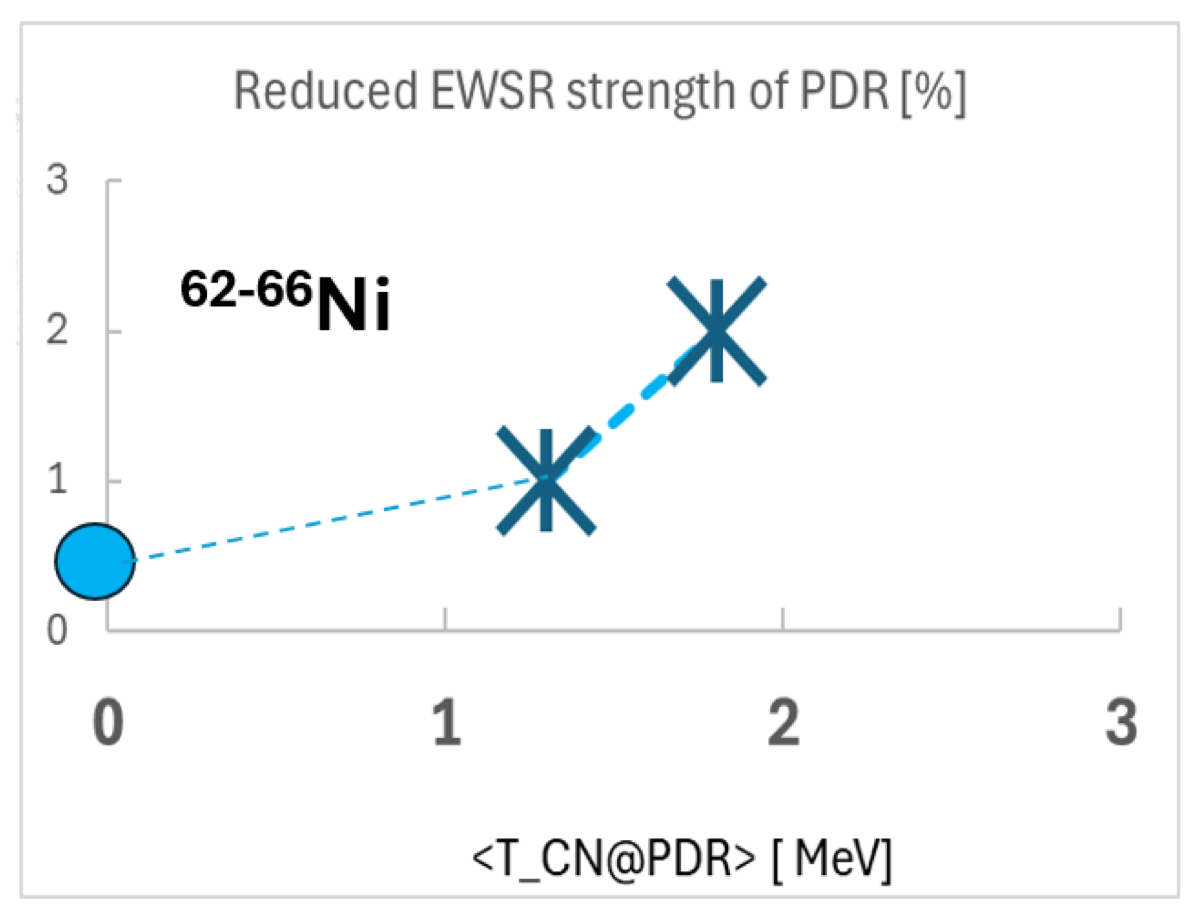
\includegraphics[width=0.6\linewidth]{graphics/Wieland.png}
    \caption{Combined preliminary results of the experiments done at CCB (circle) and IFIN (crosses). The plot shows the extra yield below the GDR for different Ni isotopes as afunction of the nuclear temperature.
}
    \label{fig:Wieland}
\end{figure}


\subparagraph{Task 2.2: Radioactive Ion Beams} \mbox{}

At \textbf{GANIL-SPIRAL2} one project focused on $^{12}$Be structure in the vicinity of different cluster thresholds, such as $^4$He, $^7$He, $^8$He by searching for narrow resonances using ACTAR-TPC detector. Second project focused at indirectly quantifying $^8$Li($\alpha$,n)$^{11}$B reaction. This reaction is involved in the nucleosynthesis from the early evolutionary stage of our universe, till the starting of r-process nucleosynthesis in supernovae, collapsars and neutron star mergers. The study has been performed by understanding the compound nucleus for the reaction, the neutron-rich $^{12}$B, with the help of the resonant elastic scattering reaction $^4$He($^8$Li,$\alpha$)$^8$Li.

At \textbf{GSI/FAIR} experiments using FRS recorded a comprehensive dataset for projectile-fragmentation products (Z = 82 to 89) from $^{238}$U on a Be target, providing essential data to refine fragmentation models and support future NUSTAR experiments. ESR has been used for investigating the rare double-gamma decay mode in 0$^+$$\rightarrow$0$^+$ transitions; this study measured isolated double-photon decays in $^{72}$Ge, and compared the two-photon decay in $^{98}$Zr and $^{98}$Mo to assess whether enhanced transition rates depend on nuclear structure, and measures of de-excitation probabilities over a wide energy range in excited $^{238}$U and $^{239}$U. For the first time, simultaneous measurements of fission, gamma, and multi-neutron emission (up to three neutrons) were achieved in a storage ring setting. R3B setup has been used for commissioning of key detectors (CALIFA, Si-tracker FOOT, NeuLAND). Cross-section measurements for (p,pd) reactions on various carbon isotopes were performed indicating the presence of strongly correlated neutron-proton pairs, with quasi-deuteron behavior influencing nucleon “dressing” in the nuclear medium. DESPEC gathered spectroscopic data around N=126 shell closer, a critical region for r-process nucleosynthesis, where new level schemes and transition probabilities help benchmark models describing the interplay of single-particle orbitals and collective excitations in heavy nuclei relevant for the astrophysical sites. FRS Ion Catcher has been used in three different experiments. A proof-of-principle study using slowed-down uranium beams in a Cryogenic Stopping Cell demonstrated that multi-nucleon transfer (MNT) reactions can produce neutron-rich isotopes (A $\approx$ 160–250). MNT products were successfully extracted and identified with the MR-TOF mass spectrometer, paving the way for future RIB production at Super-FRS (cf. \url{https://doi.org/10.1016/j.nuclphysa.2025.123041}). Also focusing on exotic nuclei from Br to Rh, this study addresses issues such as isospin symmetry breaking, the Wigner effect, and unexpected mass discrepancies (e.g., $^{70}$Br). The FRS Ion Catcher, combined with a $^{107}$Ag fragmentation beam and SIS-18 accelerator mode, delivered precise mass measurements, essential for validating nuclear models and rp-process calculations. EXPERT detector, using a $^9$C beam, probes Thomas-Ehrman shifts in mirror pairs (e.g., $^5$H-$^5$Be, $^6$H-$^5$B, $^7$H-$^7$C) and measures decay energies, widths, and half-lives (down to picoseconds) via multi-particle angular correlations. Upgraded high-rate tracking detectors have enabled high-statistics data collection, allowing for improved measurements of nuclear state widths and the identification of novel multi-proton decay mechanisms.

At \textbf{JYFL}, by using a new beta detector at IGISOL made at NCNR (Swierk/Poland), trap-assisted decay spectroscopy of very neutron-rich Rh and Pd isotopes has been performed. An interesting experiment used a reaction of deuterons on $^{242}$Pu target(s), with the goal of producing both ground states and fission isomers in $^{240,242}$Am. Set of silicon detectors were installed in the switchyard, to be used for measuring alpha activity as well as fission fragments from the decay of the isomeric states. Operated in a “duty cycle mode”, with activity monitored in the switchyard as well as beam injected into the RF cooler, either for the MR-TOF or for JYFLTRAP. The latter allowed for separation of $^{242}$Am from the target $^{242}$Pu material. Half-lives were measured, total kinetic energy of the FFs as well as the excitation energy of $^{242f}$Am with the MR-TOF. Trap-assisted decay spectroscopy of fission fragments has been performed using a beta detector connected to a tape station and surrounded by a coaxial Ge and two large BeGe detectors. This setup allowed the collection of gamma-ray transitions with energy below 20 keV in A=115 isobars region. Another project focused on neutron-deficient Ag isotopes using collinear laser spectroscopy to provide a comprehensive data set that can be used to establish a precise and accurate reference quadrupole moment for the whole Ag chain. Combined with state-of-the-art atomic calculations the aim is to investigate the consistency of quadrupole moments deduced using atomic and solid-state crystal coupling constants. A second motivation was to determine the hyperfine anomaly in Ag, which reflects changes in the distribution of nuclear magnetization. 

At \textbf{CERN/ISOLDE} several experiments addressed very topical physics in nuclei around the $^{132}$Sn double shell closure. The $^{132}$Sn(d,p) reaction has underpinned the scientific cases of many different radioactive ion beam facilities, but only a single measurement existed from more than 15 years ago before a recent ISOLDE study. This experiment studied the reaction with around ten times the intensity of $^{132}$Sn, with a higher beam energy, and with a novel spectrometer giving much improved resolution. This revealed population of $all$ the valence single-neutron orbitals for the first time and their single-particle content has been deduced, establishing them all as carrying “full” single-particle strength. In parallel, $\beta$-delayed neutron decay studies at ISOLDE have also populated the 13/2$^+$ state, with even higher energy resolution. These data on a “simple”, but exotic, nuclear system will be very impactful as they can be used in shell-model calculations of wide regions of medium-mass nuclei. The collectivity of states in this region has also been probed in Coulomb-excitation measurements of $^{130}$Sn during this period. Also using post-accelerated beams, the reaction $^{61}$Ga(d,p) was used to populate the mirror nucleus of $^{62}$Zn, an important nucleus for the astrophysical rp-process. Mirror energy differences for high-spin states in the sdpf shell were probed in a measurement of $^{39}$K(d,p) and a search was made for rotational bands at high excitation with the same beam using a $^7$Be beam. On the low-energy side of the facility, studies of laser spectroscopy have continued with measurements across many chains of nuclides, including Mg, Ca, Sb, Lu, Tm, Au and Hg isotopes. The measurements of the hyperfine structure of neutron-rich Ca isotopes are of note, shedding light on the nature of exotic shell closures and performed using a new technique that allows measurements of isotopes produced at intensities as low as 1 ion per second. Similarly, laser spectroscopy of Mg isotopes, which probed the island of inversion, demonstrated another successful new technique where ions were trapped in a mass-resolving time-of-flight spectrometer, allowing improvement in sensitivity as the laser light can probe the same nucleus very many times. Work on radioactive molecules was continued by several experimental runs, including studies of electron photo-detachment from RaF$^-$. A high statistics run was performed on the WiSARD experiment looking at non-standard model currents in weak decays using $\beta$-delayed proton emitters. Nuclear techniques were employed to characterise a number of novel materials, which included perovskites that are potentially important for novel solar cells, vanadium-based materials that have important applications in batteries, indium-gallium nitride semi-conductors, quantum colour centers in diamond that may have application as q-bits, ferroic systems such as lithium niobate that is important in piezo-electrics, and other functional materials.

Main highlights achieved by user groups in the Task 2.2 were following:

%Several experiments addressed very topical physics in nuclei around the $^{132}$Sn double shell closure 
At CERN/ISOLDE the $^{132}$Sn(d,p) reaction has underpinned the scientific cases of many different radioactive ion beam facilities, but only a single measurement existed from more than 15 years ago before a recent ISOLDE study. This experiment studied the reaction with around ten times the intensity of $^{132}$Sn, with a higher beam energy, and with a novel spectrometer giving much improved resolution. This revealed, for the first time, \textbf{population of all the valence single-neutron orbitals and their single-particle content}, establishing them all as carrying “full” single-particle strength (cf. Fig.~\ref{fig:ISOLDE_Highlight_1}). 

\begin{figure}[!h]
    \centering
    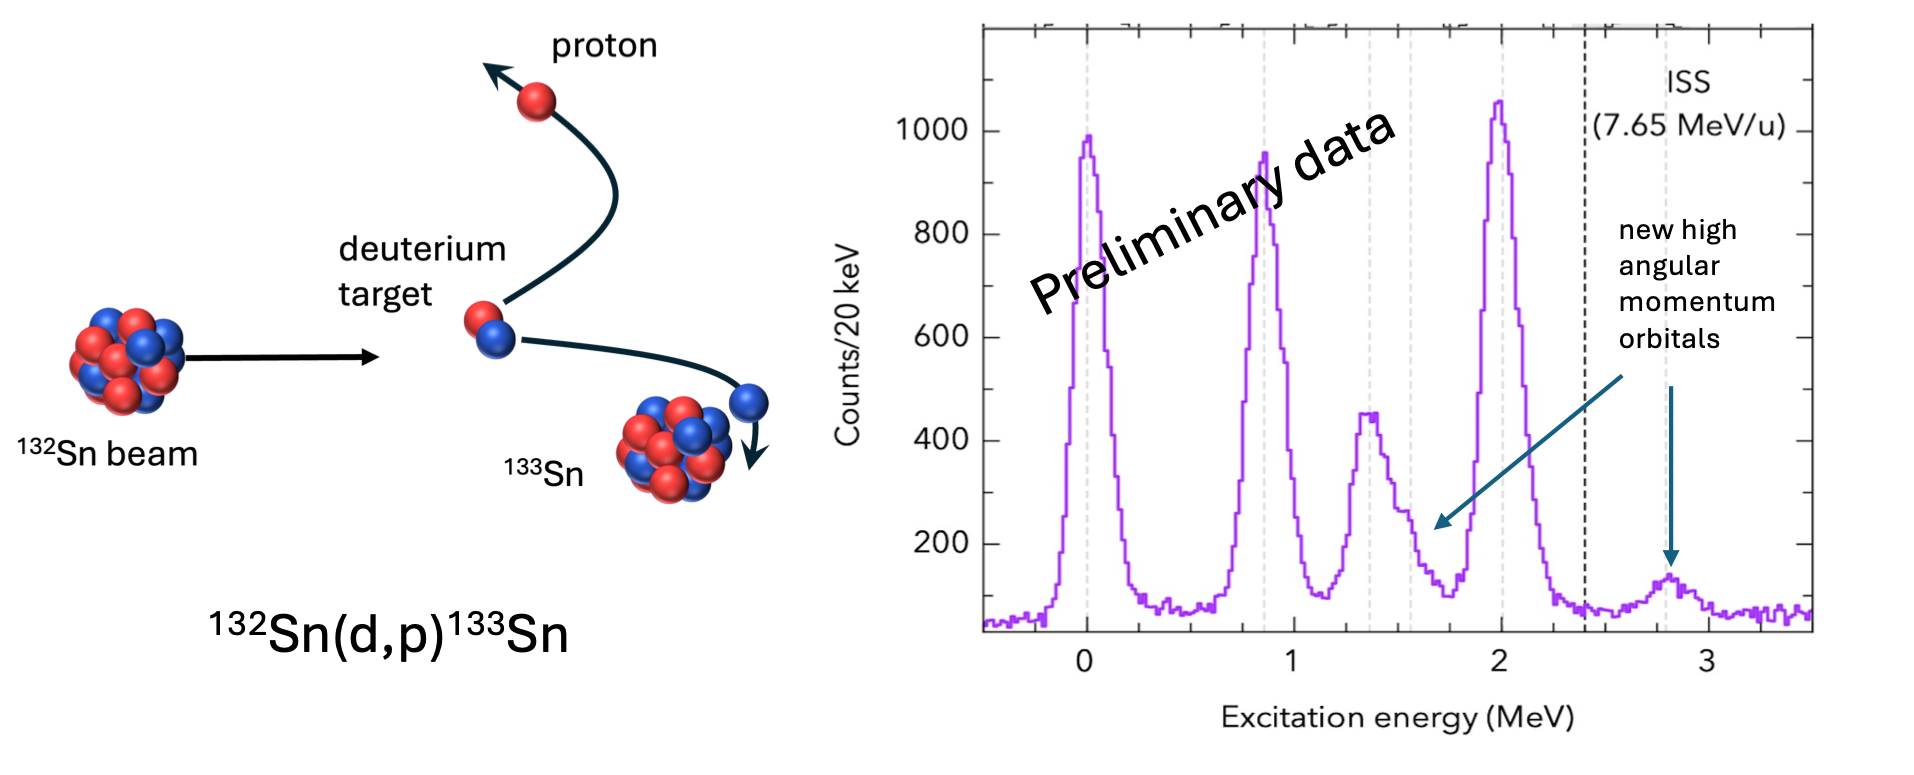
\includegraphics[width=0.9\linewidth]{graphics/ISOLDE_highlight_1.png}
    \caption{Left: A cartoon showing the mechanism for a direct (d,p) reaction.
Right: A preliminary excitation spectrum for $^{133}$Sn showing peaks corresponding to the single-neutron states outside the N=132 core.
}
    \label{fig:ISOLDE_Highlight_1}
\end{figure}

Another project at GANIL/SPIRAL2 studied the \textbf{$^{12}$Be structure in the vicinity of different cluster thresholds}, such as $^4$He and $^8$He clusters using ACTAR-TPC detector (see Fig.~\ref{fig:2alpha_cluster}). 

\begin{figure}[!h]
    \centering
    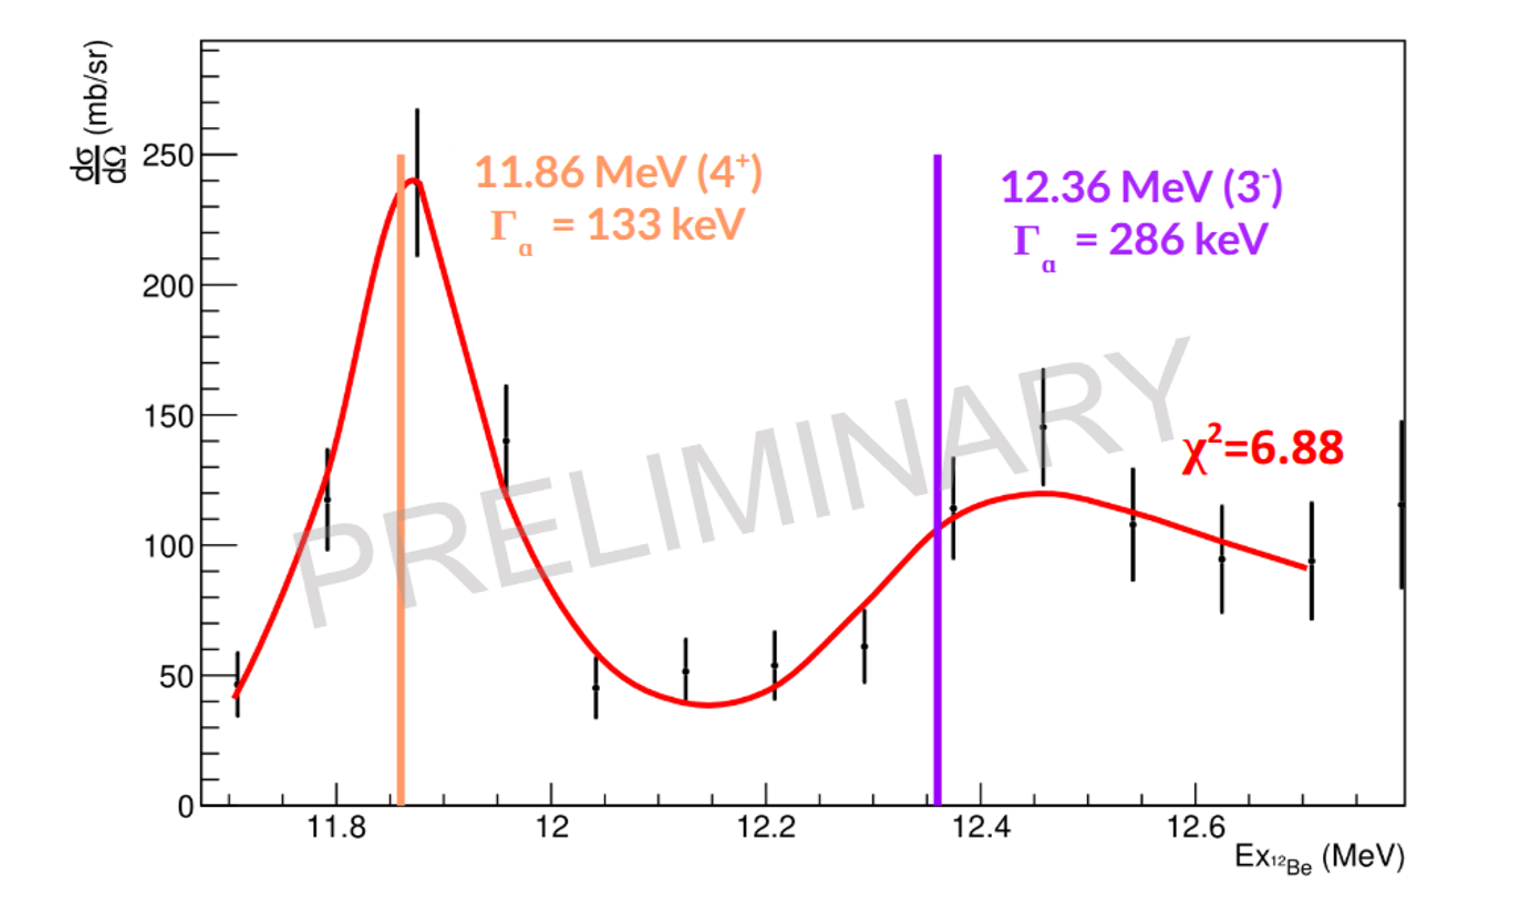
\includegraphics[width=0.6\linewidth]{graphics/2alpha_cluster.png}
    \caption{Two alpha cluster structure observed in $^{12}$Be by observing resonances in the resonance elastic scattering reaction $^4$He($^8$He,$\alpha$)$^8$He.The dark dots represents the experimental results, the red curve shows the quality of the theoretical decomposition of the results, while the violet and orange lines show the position of the cluster structure in $^{12}$Be.
}
    \label{fig:2alpha_cluster}
\end{figure}

In the project studied at JYFL joined a large collaboration from Spain (Valencia) and France (Subatech) at beta spectrometer after JYFLTRAP. This beta spectrometer has been used to directly measure the \textbf{shape of the beta spectrum of several fission fragments}. The motivation is connected to how well we understand the measured antineutrino spectrum from reactors.
%This was an excellent beam time, following on from an earlier run in 2022. Experimental improvements meant that the yields as well as the overall transmission (between 25-60\%) from the switchyard to the beta spectrometer were excellent. 
In total, around 14 cases of interest (including references) were measured, with 1 TB of data collected. These data will be sufficient to satisfy the needs of a large number of doctoral researchers in the near future.


\subparagraph{Task 2.3: Neutron Beams} \mbox{}

At the \textbf{n\_TOF} in CERN one project explored \textbf{new fission modes in lighter nuclear systems}, particularly cerium isotopes around atomic number 60 (Neodymium). Three other projects concentrated on neutron capture cross-section measurements for isotopes of Erbium and Neodymium (see Fig.~\ref{fig:n_TOF-146Nd})  improving accuracy in existing data. One of them specifically aimed to measure the $^{238}$U(n,$\gamma$) cross-section. Additionally, two projects investigated innovative techniques: measured neutron fluence using diamond detectors and testing the performances of a mixed array of HPGe and LaBr$_3$(Ce) detectors in beam.


\begin{figure}[!h]
    \centering
    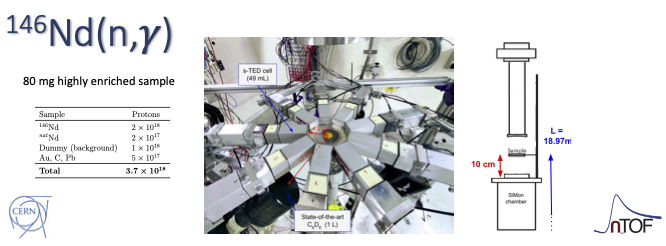
\includegraphics[width=1.0\linewidth]{graphics/n_TOF-146Nd.png}
    \caption{s-TED detector setup used at n\_TOF for the $^{146}$Nd(n,$\gamma$) reaction cross section measurement, one of the seven TA experiments executed with the EURO-LABS project support.}
    \label{fig:n_TOF-146Nd}
\end{figure}

In \textbf{CLEAR-CNA} a notable experiment was performed, measuring actinides in Baltic seaweed, characterizing novel targets for astrophysics, and assessing the impact of radioactivity from nuclear facilities. 

At the \textbf{ALTO} facility, one LICORNE project refined fast neutron tomography techniques and studied radiation damage in LaBr$_{3}$ crystals under high neutron fluence, crucial for the NUMEN project. 

At \textbf{GANIL}'s NFS facility, two key experiments investigated gas production in chromium and copper, respectively. Both projects utilized advanced experimental setups to measure double-differential cross sections for neutron-induced reactions, contributing valuable data for future fusion plant simulations and nuclear reaction models.

\subparagraph{Task 2.4: Theoretical Support} \mbox{}

The theoretical support offered at \textbf{ECT*} covered a broad range of subjects in various workshops, which were characterized by a high degree of interaction and collaboration among participants. At a fundamental level, progress has been achieved in the theoretical description of how quarks and gluons interact to give rise to the nuclear forces that shape the structure of nuclei. Strategies were mapped out to probe generalized parton distributions through novel exclusive processes and to use Lee-Yang singularities to determine the critical point of the QCD deconfinement transition. It was clarified that while global equilibrium in the QCD plasma probed in heavy-ion reactions is unique and independent of the pseudo-gauge choice, the definition of local equilibrium differs in quantum kinetic theory and quantum statistical field theory and is furthermore susceptible to a pseudo-gauge ambiguity. New directions have been charted for an {\it ab initio} development of optical potentials, including the Dispersive Optical Model and Green’s Function Theory, which are essential for the extraction of nuclear properties from lower-energy reactions. The takeaways for stellar dynamics, sensitivity studies, and astrophysical observations (including the determination of elemental abundances in stars) were extracted from key astrophysical reactions studied at facilities such as LUNA (Italy), JUNA and LEAF (China), CASPAR (USA), STELLA (France), Felsenkeller (Germany), and various large RIB installations. A Doctoral Training Program further enhanced the training of early career researchers in nuclear astrophysics, in particular the interplay between theory, experiment, and observations in the determination of the neutron-matter equation of state, as well as its impact on the neutron-star dynamics, neutrino emission, nucleosynthesis, and (gravitational and electromagnetic) signals from mergers. A separate workshop probed the extent to which these signals could provide a smoking gun for the presence of hyperons in neutron stars, which is strongly influenced by two- and three-body hyperon-nucleon forces inferred from information on hypernuclei. Nuclear theorists informed experimentalists of the specific data that is needed to benchmark and further develop models for neutrino-nucleus interactions, as needed for the analysis of next-generation oscillation experiments. Novel opportunities were identified for the determination of electric dipole moments, a sensitive probe of physics beyond the Standard Model of particle physics, such as a radioactive isotope/molecule program that could be envisioned at PSI (Switzerland). The nuclear physics opportunities of new high-power laser facilities, such as ELI-NP (Romania) have also been explored. Discussions on modern algorithms in machine learning and data analysis (from medical physics to research with accelerators and in underground laboratories) identified generative models at the LHC (Switzerland) as a promising strategy to reduce computing time, though challenges in deployment were acknowledged.

Overall, all of these initiatives of WP2 highlight significant advancements in nuclear physics research and the importance of collaborative efforts between theorists and experimentalists across various facilities.
%
% 
\subparagraph{Work Package 3 - Access to RIs for Accelerators} \mbox{}
\label{sec:wp3_scientific_output}
% \todo{Scientific output of WP.}


The scientific projects conducted by the WP3 TA users span a wide range of research frontiers, benefiting from the unique capabilities of the facilities. Some highlights are presented below.

\textbf{\textit{Laboratory Astrophysics}} \mbox{}

The \textbf{HRMT-62} and \textbf{HRMT-64} series of experiments, conducted during P2 at the HiRadMat Facility at CERN, focuses on pioneering and high-quality R\&D utilizing the unique characteristics of the facility to conduct laboratory experiments for astroparticle research. The HRMT-62 experiment inaugurated and demonstrated the use of the HiRadMat facility to produce high-intensity, high-density, ultra-relativistic, quasi-neutral electron-positron pair beams, thereby opening up the possibility of studying the microphysics of such pair plasmas through experimental means.
In the subsequent HRMT-64 experiment, with an improved setup that included a secondary target and a magnetic collimating system, the focus was on studying the emergence of magnetic fields associated with the growth of filamentation instabilities. This was done by observing the propagation of collimated relativistic pair-plasma beams through ambient plasma, an analogue for the propagation of astrophysical pair jets through the intergalactic medium.

The results of the experiments were published in well known scientific journals with high impact, triggering the attention of hte community. Up to-date, 5 peer-reviewed articles have been written, 3 of them published in or submitted to Nature, all citing the EURO-LAB support. In total, 14 press releases have been done by the collaborating institutes, including 2 from CERN (bulletin \& courrier). It worth noting that the articles have a high ``attention score'', of 260: 99th percentile of the 329,972 tracked articles of a similar age in all journals. The key scientific result from HRMT-64, only made possible with the EURO-LABS support, was the first-time measurement of the magnetic fields produced by plasma instabilities using a Faraday rotation, seen in Figure~\ref{fig:hiradmat_mag_field_plasma}.
\begin{figure}[H]
    \centering
    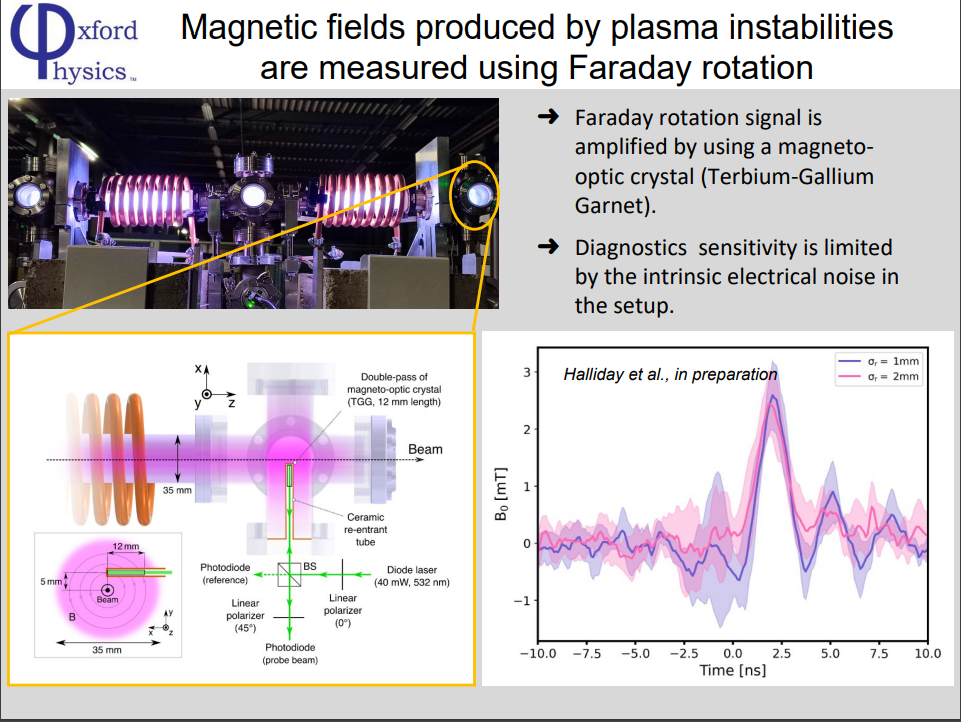
\includegraphics[width=0.75\linewidth]{graphics/HRMT_64_magnetic_field.png}
    \caption{HRMT-64, with the EURO-LABS support measured for first time the magnetic fields produced by plasma instabilities using a faraday rotation in HiRadMat. Courtesy: Prof. G. Gregori, Univ. of Oxford.}
    \label{fig:hiradmat_mag_field_plasma}
\end{figure}

\textbf{\textit{Material R\&D}} \mbox{}

\textbf{HRMT-66} was a novel experiment that pushed forward our current knowledge of material limits, particularly for the often used Glassy Carbon and Beryllium, along with a first-time irradiation of Si$_{3}$N$_{4}$ in order to investigate its exact damage threshold. This is very important for the cooling section of a future muon collider. A photo from the results is shown in Figure~\ref{fig:hiradmat_Si3N4} for Si$_{3}$N$_{4}$ and in Figure~\ref{fig:hiradmat_GC} for Glassy Carbon. The support of EURO-LABS was extremely important since FLUKA simulations were absolutely necessary for the evaluation of the damage mechanisms and precence at CERN was vital for some of the collaborators of the experiment.

\begin{figure}[!h]
    \centering
    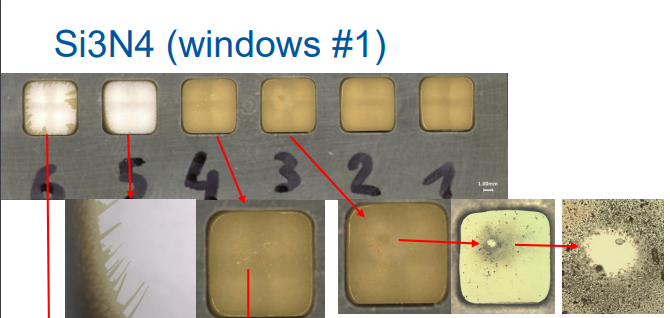
\includegraphics[width=0.85\linewidth]{graphics/hiradmat_si3n4.png} \\
    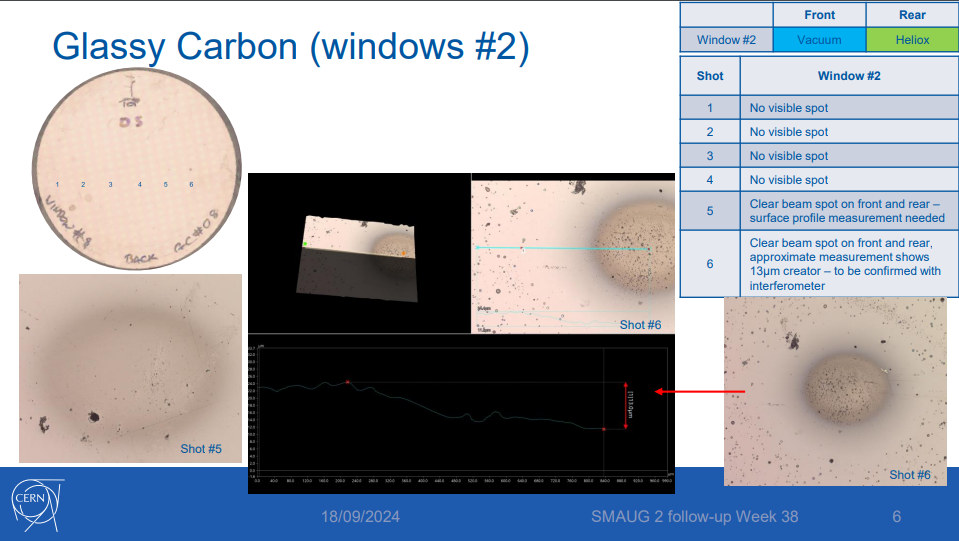
\includegraphics[width=0.85\linewidth]{graphics/hiradmat_GC.png}

    \caption{Top : Beam impact on Si3N4 windows during HRMT-66 experiment. The clear beam spot can be seen in shot \#6 including a small crater. Bottom : Results from HRMT-66 experiment on Glassy Carbon. . (Courtesy: A. Harrison, CERN)}
    \label{fig:hiradmat_Si3N4}
\end{figure}


\textbf{\textit{Instrumentation R\&D}} \mbox{}
\textbf{HRMT-55} is a collaboration between CERN and ESS, to develop a new generation of ionization chambers able to work in high intensify environments, of interest for both Organizations.

Figure~~\ref{fig:hiradmat_IC_response} shows the response of different ionisation chambers (IC) tested for increasing beam intensity. The results indicate a close-to-linear detector performance for all , however with large variations in slope between them. 
\begin{figure}[!h]
    \centering
    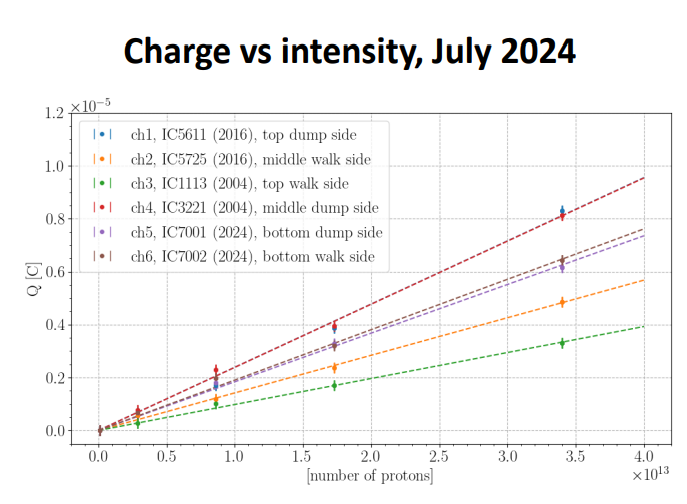
\includegraphics[width=0.8\linewidth]{graphics/hiradmat_IC_response.png}
    \caption{Response (C) of the different ionization chambers tested in HRMT-55. The difference in the slope needs to be understood in detail in a follow-up experiment (HRMT-71) planned for 2025. (Courtesy. S. Grishin, ESS)}
    \label{fig:hiradmat_IC_response}
\end{figure}
This is, for the moment, a puzzling result; therefore, a follow-up experiment \textbf{HRMT-71} is planned for 2025 to further investigate the underlying reasons.

\textbf{R\&D for future accelerators - I}
\todo{PIP-II cavities in SUPRATECH-MACHAFILM}

\textbf{\textit{R\&D for future accelerators}} \mbox{}

Particle accelerators and colliders must cope with a large amount of synchrotron radiation (SR) power being deposited on the vacuum chamber walls.
Photo-stimulated desorption (PSD) leads to increasing pressure and high heat load and is therefore to be investigated using new types of a number of beam screen and vacuum chamber prototypes. The results of this study will be critical for the design of future high-energy hadron colliders such as FCC-hh, in addition this research has potential implications also for the near future of the LHC. 
\begin{figure}[H]
  \centering
  \begin{minipage}[c]{0.45\textwidth}
    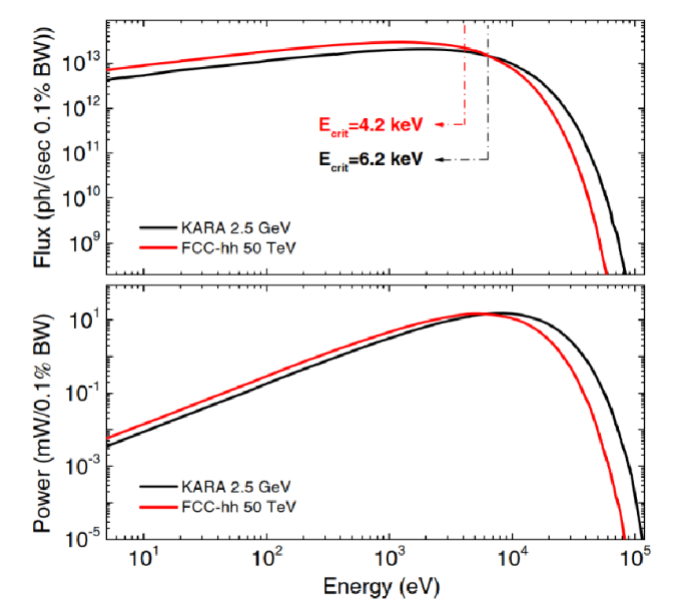
\includegraphics[width=\textwidth]{graphics/wp3-KIT_FCCphotons.png}
  \end{minipage}%
  \hfill
  \begin{minipage}[c]{0.5\textwidth}
    \vspace*{\fill}
    \captionof{figure}{Comparison of the photon flux (top) and power (below) of the FCC-hh at \SI{50}{TeV} proton beam energy in comparison with KARA's at its nominal \SI{2.5}{GeV} electron energy for user %operation. Calculations were performed with SYNRAD+~\footnote{see: L. A. González et al. DOI: 10.1103/Phys.Rev.Accel.Beams 22, 083201, and L. A. González et al. (2021) Phys.Rev.Accel.Beams 24, 113201}
    }
    \label{fig:yourlabel}
    \vspace*{\fill}
  \end{minipage}
\end{figure}

During the EU-project EuroCirCol CERN and KIT realized the BESTEX beamline of CERN at the KIT light source. The storage ring of the KIT light Source is the synchrotron KARA delivering similar spectra as expected at the FCC.

CERN installed a residual gas analyser in the central part of the BESTEX test chamber  before the start of the FCC beam screen prototype experiment (no.5, with saw-tooth profile to decrease synchrotron radiation photon scattering) in period P1 (EURO-LABS-KIT-KARA-2023-01). In period P2 this prototype was exchanged by the new beam-screen prototype no. 6 with amorphous carbon coating (aC). aC is a stable and inert material, deposited via sputtering techniques onto the internal wall of a circular tube (carried out at CERN).  The main feature of aC is its extremely low secondary electron yield, which is necessary to avoid electron cloud instability in accelerators with positively charged beams. In the long-term experiment at KARA (EURO-LABS-KIT-KARA-2023-03), the beam-screen prototype no. 6 was irradiated at a flat angle of incidence and cooled with LN2. The increase in pressure was measured. In addition, the composition of the species outgassing from the beam screen was determined at CERN's BESTEX beamline at KARA. The experiment began installation in August 2023 and the prototype was irradiated with over 480 KARA synchrotron light until the first quarter of 2024. The prototype is still installed in BESTEX and is waiting to be exchanged for the next one, which is currently being prepared
\begin{figure}[!h]
    \centering
    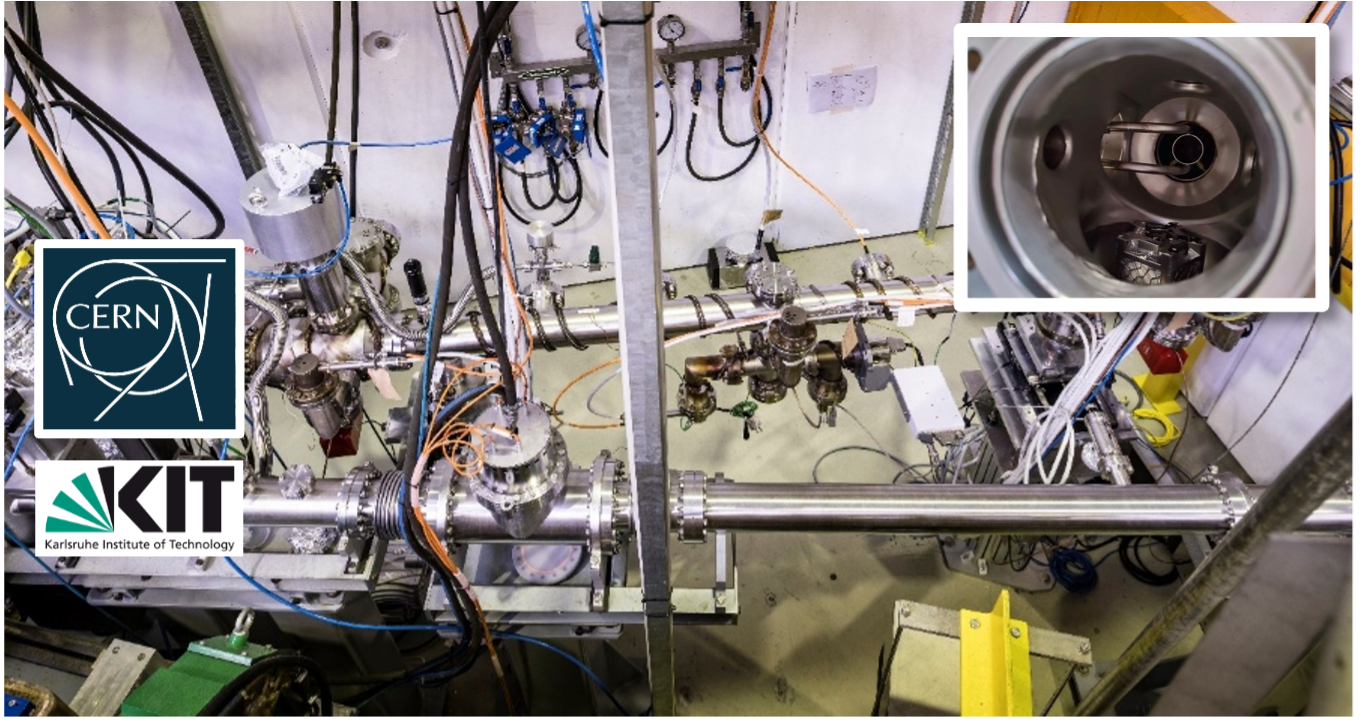
\includegraphics[width=0.75\linewidth]{graphics/wp3-KIT_BESTEX.png}
    \caption{CERN installed the BESTEX beamline at KARA since 2019 (EU project EuroCirCol). BESTEX was used for up to now two actual TA experiments within EURO-LABS. A goal is the exploration of the vacuum performance of the FCC-hh beam screen to protect the cold superconducting magnets from the 
direct irradiation high-power SR photon beams.
}    
    \label{fig:kit_bestex}
\end{figure}

The KARA experiment (EURO-LABS-KIT-KARA-2023-04) of the University Lille aimed to observe, understand and control the ultrafast self-organisation of relativistic electron bunches in accelerator facilities. A central goal is to master the emission of giant terahertz (THz) pulses in coherent synchrotron radiation (CSR), which is a proposal for new THz sources. Another important goal was the improvement of novel ultrafast observation instruments. KARA is one of the only electron storage rings in the world where the shape of relativistic electron bunches can be directly ‘studied’ in a storage ring facility. The techniques of chaos control (feedback control of periodic orbits) for achieving stable THz-CSR emissions, which the team at the University of Lille had already successfully tested at the SOLEIL synchrotron, were transferred to the KIT light source KARA, and the results have thus been compared between the machines and with theory. At KARA, the opportunity was taken to observe the development of the longitudinal bunch profile in real time with the help of the existing electro-optical near-field setup. In this experiment, an advanced control loop from chaos control theory was implemented on a fast FPGA board to control the amplitude of one of the two main radiofrequency (RF) cavities in the electron storage ring KARA at KIT. The CSR emission of THz power at high level was stabilised to control the micro-bunching instability. The fast Schottky diodes in the KIT-IR2 beamline at KARA were used and the THz power was measured in real time with the high-speed data acquisition card KAPTURE developed by KIT.
\begin{figure}[H]
    \centering
    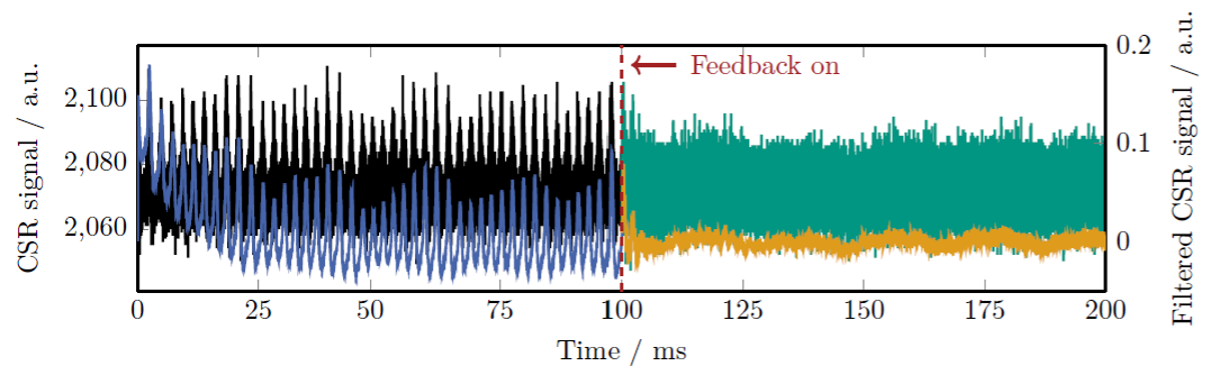
\includegraphics[width=0.75\linewidth]{graphics/wp3-KIT_CSRsignal.png}
    \caption{The CSR signal was measured with a fast Schottky diode (at a KIT infrared beam line). After \SI{100}{ms} the team of the University Lille (F) switched on the FPGA-based feedback loop. For better visibility, the raw signal (black, left \& green, right) was filtered (blue, left \& orange, right) to remove the fast sinusoidal fluctuation. Suppression of the sawtooth outburst fluctuation variance by a factor of 28 in the CSR emission at the KARA electron storage ring, after switching on the FPGA-based feedback loop developed by the PhLAM team of University Lille. The fast CSR fluctuations are still present after the feedback is switched on, leading to a stabilization of the THz emission. Publication in preparation.}    
    \label{fig:kit_csr}
\end{figure}

FCC-ee precision physics measurements require an accurate and precise determination of the centre-of-mass collision energy, which can be obtained from the beam energies. Since the depolarisation frequency is directly proportional to the beam energy, a promising way to determine this energy is to depolarise transversely polarised packets. This resonant depolarisation (RDP) has long been used in KARA whereby the resonance frequency is measured via the change in the Touschek lifetime. At KARA, a first RDP measurement campaign (EURO-LABS-KIT-KARA-2023-05) with numerous scan settings and bundle configurations was carried out to investigate how this technique could be applied at FCC-ee, in particular the sensitivity to parameters such as the scan speed of the depolariser and the scan velocity. The measurement campaign was successful and the users at CERN expressed interest in carrying out another measurement campaign at a later target point.
\begin{figure}[H]
    \centering
    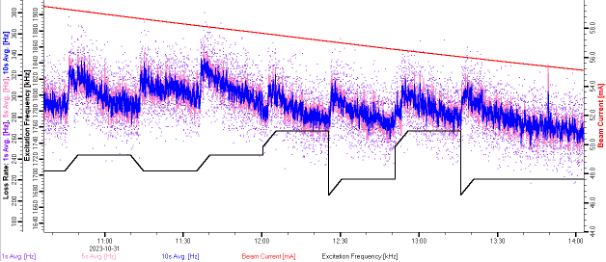
\includegraphics[width=0.75\linewidth]{graphics/wp3-KIT_RDPscans.png}
    \caption{More than 40 successful RDP scans were realized at KARA by scanning direction up and down for scanning times of \SI{100}{s} to \SI{600}{s}, respectively}    
    \label{fig:kit_rdp}
\end{figure}

RDP results published in:
\begin{itemize}
\item FCCIS WP2-workshop, 2023-11-15, B. Härer et al.: Polarisation studies at KARA
\item and in the following IPAC papers: \\ https://doi.org/10.18429/JACoW-IPAC2024-TUPG33, \\ https://doi.org/10.18429/JACoW-IPAC2024-WEPG51, and \\ https://doi.org/10.18429/JACoW-IPAC2024-WEPR20
\end{itemize}

Bunch-by-bunch (BBB) feedback systems are essential for the realisation of ultra-low emittance rings that allow electron beams to reach high-quality states for use in synchrotron radiation light sources and colliders. Following the workshop WP7.2 of the EU project I.FAST on BBB feedback systems, which was attended by more than 40 experts on BBB systems from all over the world, the following three experiments were carried out at the request of the experts in connection with the BBB systems carried out at the KARA storage ring and at the booster synchrotron with real electron beams by operating the BBB systems installed in each of the two accelerators(EURO-LABS-KIT-KARA-2024-06). The aim of the first experiment at KARA was to manipulate the vertical beam size by exciting the betatron oscillation with the BBB system to improve the Touschek beam lifetime. The goal of this experiment was to look for common procedures for commissioning bunch-by-bunch feedback systems. The goal of the third experiment was to longitudinal kicks with the bunch-by-bunch feedback system and the stripline kicker installed in the booster synchrotron. This experiment will lead to the next step, such as longitudinal manipulation of beams to improve booster beam quality. Data and results of the three experimental topics have been shared with all interested participants, and the data analysis and subsequent discussions are ongoing. 


According to the design of the FCC, the desired mechanical alignment tolerances of the magnets are in the range of \SI{100}{\micro\meter} to \SI{150}{\micro\meter}. However, to achieve the ambitious research goals at the FCC, a low (10-20 µm) relative alignment of the quadrupoles and sextupoles is required. For this purpose, correction magnets are provided to steer the beam in the direction of the magnetic centre, which is known as beam-based alignment (BBA). The BBA must be performed for approx. 1870 quadrupoles and approx. 630 sextupoles, so in addition to the accuracy, the average time required to determine the individual magnetic offset is a key parameter for the selection of the BBA method. The development of a concept for the BBA at FCC-ee is currently based on simulations but is to be supported by proof-of-principle tests on existing machines, for which experiments were carried out at KARA (EURO-LABS-KIT-2024-KARA-07).  Strategies were successfully investigated that will significantly reduce the time required for the BBA at FCC.


\textbf{\textit{Novel detector R\&D}} \mbox{}

\begin{description}
\item[MM\_TCP]: The experiment goal was to test and validate TPC performances of two MicroMegas detectors based on a strip read out system. The resistive Micromegas chambers are frontier Micro-Pattern Gas Detectors with a planar geometry and with an amplification gap of the order of \SI{18}{\micro\meter} between the read-out (RO) PCBs and the mesh. Similar detectors have been widely used and recently installed in the muon spectrometer of one of the LHC experiment, covering a dimension of \SI{2400}{\meter\tothe{2}}.
The purpose of the test beam is to study and tune the DAQ based on APV technology in order to adapt to the acquisition window required for TPC purposes.
\begin{figure}[H]
    \centering
    \includegraphics[width=0.48\linewidth]{graphics/BTF-MMTPC2.jpeg}
    \includegraphics[width=0.48\linewidth]{graphics/BFT-MMTPC3.jpeg}
    \caption{Photo of the experimental setup in the BTF line.}    
    \label{fig:kit_rdp}
\end{figure}
Two different types of Micromegas, one of which never previously tested, have been experimentally characterized. The planned test and some other extra test have been fully acquired, with calibration and load curve in different beam configuration especially for flux and multiplicity.
The experiment resulted to be well-planned, executed smoothly, and achieved its goals. The combination of on-site and remote support, along with continuous monitoring of the system parameters, contributed to the overall success of the operation.
Experiment Duration: 1 week or 168 h (2023, 20-27 November)

\item[MICROGASTRACK]:
The experiment aimed at testing a novel micromegas gas chamber with variable high voltage which could enable both to track the secondary particles produced in the interactions and to measure the initial high intensity beam parameters. The device under test combines the functionalities of micropattern gas detectors for precise sub millimetre tracking and gas detectors for beam monitoring.

The detector that was expected to be ready for the test beam time, was unfortunately not completed in time. However, the team was able to test the MM electronics and integrate with the BTF timing and triggering. Additionally, during the beam time, a successful integration of future detector support was achieved. The team had also the possibility to test the detector electronics (APV25) and the communication with the pre-existing DAQ system
Experiment Duration: 2 weeks or 336 h (2024, 4-18 November)

\item[CALOBEAMPIX]:
The experiment goal was to test silicon pixel detectors for simultaneous measurement of electron/positron beams with two different types of detectors: calorimeter and silicon pixel detector. 

The following experimental goals were reached:
\begin{itemize}
    \item Operate simultaneously Timepix3 array and lead glass calorimer
    \item Develop threshold equalization procedure for the Timepix3 pixels
    \item Synchronized data acquisition (either online or offline) of Timepix3 and lead-glass calorimeter
    \item Calibrate the lead glass block for different beam multiplicity using the Timepix3 data
\end{itemize}
Experiment Duration: 1 week or 168 h (2024, 9-16 December)
\end{description}


%\textbf{Medical Physics R\&D}

%\begin{description}
%    \item[AI1] Artificial Intelligence readiness at CLEAR. Done, Reimbursed (A. Pollastro, 40 units)
%    \item[LUXE2] Done, reimbursed (F. Lasagni-Manghi, 40 units)
%    \item[THz] THz sources on Smith-Purcell radiation, THZ1 > Initial visit + preparation done,  will not be reimbursed (paid by Users Lab) (T. Zhang, 16 units)
%    \item[SE1] Electron collimation at CLEAR (SE1) > Done, to be reimb. (N. Delerue, D. Dauvergne, 64 units)
%\end{description}

\textbf{Applications}


\begin{itemize}
\item One-electron oxidation of S-adenosyl methionine,
\item Crosslinking of self-assembled fatty acids on copper by electron beam irradiation,
\item Effect of ionizing irradiation on dried fruits,
\item Influence of 10 MeV accelerated electrons on structure and properties of sheep wool fibres as a potential component for preparation of polymer-based composite materials
\item Irradiation engineering of biopolymer-based formulation for wound management and targeted drug delivery devices,
\item Bioactivity of irradiated foods by low energy e-beam,
\item Face masks recycling with the use of radiation technologies.
\end{itemize}
%
% 
\subparagraph{Work Package 4 - Access to RIs for Detectors} \mbox{}

WP4 is the enabler of Detector R\&D, the fundament of current and future scientific endavour. Most of its scientific output is thus hidden, displaced to the developed detectors, their implementation in experiments and the fundamental physics discoveries those experiments shall unravel. Needless to list what shall be discovered – if we knew that, there would be no need for conducting experiments.

WP4 is of vital importance for the successful completion of the HL-LHC project, the focal point of the European Strategy for Particle Physics (ESPP) in 2013 and its update in 2020. The upgrades have nearly finished their R\&D and the construction of the detectors is in full swing. There are, however, late surprises that still require verification of the solutions in the WP4 RI’s. The experiment upgrades for the LHC are amply documented in the respective Technical Design Reports (TDR) and in the Memoranda of Understanding (MoU) for the specific detectors, available on the CERN Document Server (CDS).

The shift of focus in WP4 is synchronized with the stipulations of the ECFA Detector R\&D Roadmap, serving either the medium term goals like the Higgs factory or the more distant endeavour towards the highest energy hadron collider (FCC-hh). WP4 backs up the newly set up DRD collaborations by providing them with access to top-level infrastructure needed for their detector R\&D. The more precise guideline to future facilities, e.g. which Higgs factory to build in the next decade is expected from the currently ongoing strategy process (ESPP), to be adopted by the CERN Council in early 2026.

The spectrum of DRD collaboration research activities is best illustrated in their proposals and their structuring into Work Packages and Working Groups. They follow closely the programme, set up by  the DRD Themes (DRDT) specified in the Detector R\&D Roadmap.

WP4 is delivering the services needed for detector R\&D. The resulting scientific output in terms of publications is two-fold: scientific results in instrumentation are being published in scientific journals and conference proceedings during the duration of the project. The more glorious part with the physics results of the HL-LHC experiments and their follow-ups at future colliders will, however, start emerging during the next decade and beyond, when the detectors now being tested at WP4 RIs will be put to their proper usage and deliver precious physics data.


\tsubsubsection{Virtual access (VA) activities}

\todo{Activities on VA installations}

% 1.6 Resources
%
% User of rersources
\subsection{Resources used to provide access to research infrastructures}
%\todo{For virtual or trans-national access costs reported as actual costs, include for each access provider information on how many of the person-months (PM) reported in the use of resources have been used to provide access and explain for which task}

\begin{table}[H]
% \caption{Information on the TA applications received in P2.}
\centering
\begin{tabularx}{\textwidth}{|c|c|c|X|} \hline
    \rowcolor{mycyan}
    {\bf Beneficiary} & {\bf Installation(s} & {\bf Number of PM}  & {\bf Explanation of tasks} \\ \hline
    IFJ-PAN & MeanField4Exp & 36.30 & Programming the codes, testing them and installing on the web server MeanField4Exp, maintaining the VA facility and administrating accesses and security” (WP2.4.2)\\ \hline
    IFJ-PAN & AIC-144 & 3.00 & Supporting experiments on irradiation of materials (WP4)\\ \hline
    U. Milano & Structure4Exp & 16.80 & Programming the codes, testing them and installing on the web server Structure4Exp, maintaining the VA facility and administrating accesses and security (WP2.4.2)\\ \hline 
   USE & Reaction4Exp & 3.27 + 22.00 & Programming the codes, testing them and installing on the web server Reactions4Exp, maintaining the VA facility and administrating accesses and security at the main entry point Theo4Exp (WP2.4.2). (Note: 3.72 PM is not reported part of PMs in P1 - it was reported 7.2 instead of 10.47) \\ \hline
   CNRS & SUPRATECH & - & - \\ \hline
   ITAINNOVA & EMCLab & - & - \\ \hline
   UU & GERSEMI, HNOSS & - & - \\ \hline
   CEA & Synergium & - & - \\ \hline
   INCT & RAPID & - & - \\ \hline
   
\end{tabularx}
\label{tab:resources}
\end{table}

%%%%%%%%%%%%%%%%%%%%%%%%%%%%%%%%%%%%%%%%%